%%%%%%%%%%%%%%%%%%%%%%%%%%%%%%%%%%%%%%%%%%%%%%%
%
% Template per Elaborato di Laurea
% DISI - Dipartimento di Ingegneria e Scienza dell’Informazione
%
% update 2015-09-10
%
% Per la generazione corretta del 
% pdflatex nome_file.tex
% bibtex nome_file.aux
% pdflatex nome_file.tex
% pdflatex nome_file.tex
%
%%%%%%%%%%%%%%%%%%%%%%%%%%%%%%%%%%%%%%%%%%%%%%%


% formato FRONTE RETRO
\documentclass[epsfig,a4paper,11pt,titlepage,twoside,openany]{book}
\usepackage{epsfig}
\usepackage{plain}
\usepackage{setspace}
\usepackage[paperheight=29.7cm,paperwidth=21cm,outer=1.5cm,inner=2.5cm,top=2cm,bottom=2cm]{geometry} % per definizione layout
\usepackage{titlesec} % per formato custom dei titoli dei capitoli

\usepackage{xcolor}%TO DO RIMUOVI
\usepackage{listings} %
\usepackage{minted} %
\usepackage{graphicx}%
\usepackage{caption}%
\usepackage{subcaption}%
\usepackage{makecell}%

%%%%%%%%%%%%%%
% supporto lettere accentate
%
%\usepackage[latin1]{inputenc} % per Windows;
\usepackage[utf8x]{inputenc} % per Linux (richiede il pacchetto unicode);
%\usepackage[applemac]{inputenc} % per Mac.

\singlespacing

\usepackage[italian]{babel}

\begin{document}

  % nessuna numerazione
  \pagenumbering{gobble} 
  \pagestyle{plain}

\thispagestyle{empty}

\begin{center}
  \begin{figure}[h!]
    \centerline{
\psfig{file=marchio_unitrento_colore_it_202002.eps,width=0.6\textwidth}}
  \end{figure}

  \vspace{2 cm} 

  \LARGE{Dipartimento di Ingegneria e Scienza dell’Informazione\\}

  \vspace{1 cm} 
  \Large{Corso di Laurea in\\
    Informatica
    %Ingegneria dell'Informazione e delle Comunicazioni
    %Ingegneria dell'Informazione e Organizzazione d'Impresa
    %Ingegneria Elettronica e delle Telecomunicazioni
  }

  \vspace{2 cm} 
  \Large\textsc{Elaborato finale\\} 
  \vspace{1 cm} 
  \Huge\textsc{Progettazione e sviluppo di un software gestionale\\}
  %\Large{\it{Sottotitolo (alcune volte lungo - opzionale)}}


  \vspace{2 cm} 
  \begin{tabular*}{\textwidth}{ c @{\extracolsep{\fill}} c }
  \Large{Supervisore} & \Large{Laureando}\\
  \Large{Chiar.mo Prof.}\\\Large{Paolo Bouquet}& \Large{Alessandro Lorenzi}\\
  \end{tabular*}

  \vspace{2 cm} 

  \Large{Anno accademico 2022/2023}
  
\end{center}



  \clearpage
 
%%%%%%%%%%%%%%%%%%%%%%%%%%%%%%%%%%%%%%%%%%%%%%%%%%%%%%%%%%%%%%%%%%%%%%%%%%
%%%%%%%%%%%%%%%%%%%%%%%%%%%%%%%%%%%%%%%%%%%%%%%%%%%%%%%%%%%%%%%%%%%%%%%%%%
%% Nota
%%%%%%%%%%%%%%%%%%%%%%%%%%%%%%%%%%%%%%%%%%%%%%%%%%%%%%%%%%%%%%%%%%%%%%%%%%
%% Sezione Ringraziamenti opzionale
%%%%%%%%%%%%%%%%%%%%%%%%%%%%%%%%%%%%%%%%%%%%%%%%%%%%%%%%%%%%%%%%%%%%%%%%%%
%%%%%%%%%%%%%%%%%%%%%%%%%%%%%%%%%%%%%%%%%%%%%%%%%%%%%%%%%%%%%%%%%%%%%%%%%%
  \thispagestyle{empty}

\begin{center}
  {\bf \Huge Ringraziamenti}
\end{center}

\vspace{2cm}

\noindent
\newline
\emph{
Ringrazio il mio relatore, il Prof. Paolo Bouquet, per la sua disponibilità, il supporto e l'attenzione fornita durante la stesura dell'elaborato, per i consigli e le conoscenze trasmesse in questo periodo.\\
\newline
Un grazie a tutto il personale dell'azienda Dream S.R.L. per avermi dato la possibilità di svolgere il mio tirocinio in un luogo interessante e dinamico, e per l’esperienza preziosa svolta.\\
\newline
Il ringraziamento più grande e importante va ai miei genitori che mi hanno sempre appoggiato, sostenuto e incoraggiato. Mamma e papà: questo elaborato è dedicato a voi. La vostra presenza, la comprensione e tutti gli insegnamenti dati sono stati fondamentali per avermi fatto diventare chi sono oggi; senza di voi non sarei mai potuto arrivare a questo importante traguardo. Grazie. \\
}

  \clearpage
  \pagestyle{plain} % nessuna intestazione e pie pagina con numero al centro

  
  % inizio numerazione pagine in numeri arabi
  \mainmatter

%%%%%%%%%%%%%%%%%%%%%%%%%%%%%%%%%%%%%%%%%%%%%%%%%%%%%%%%%%%%%%%%%%%%%%%%%%
%%%%%%%%%%%%%%%%%%%%%%%%%%%%%%%%%%%%%%%%%%%%%%%%%%%%%%%%%%%%%%%%%%%%%%%%%%
%% Nota
%%%%%%%%%%%%%%%%%%%%%%%%%%%%%%%%%%%%%%%%%%%%%%%%%%%%%%%%%%%%%%%%%%%%%%%%%%
%% Si ricorda che il numero massimo di facciate e' 30.
%% Nel conteggio delle facciate sono incluse 
%%   indice
%%   sommario
%%   capitoli
%% Dal conteggio delle facciate sono escluse
%%   frontespizio
%%   ringraziamenti
%%   allegati    
%%%%%%%%%%%%%%%%%%%%%%%%%%%%%%%%%%%%%%%%%%%%%%%%%%%%%%%%%%%%%%%%%%%%%%%%%%
%%%%%%%%%%%%%%%%%%%%%%%%%%%%%%%%%%%%%%%%%%%%%%%%%%%%%%%%%%%%%%%%%%%%%%%%%%

    % indice
    \tableofcontents
    \clearpage
    
    
          
    % gruppo per definizone di successione capitoli senza interruzione di pagina
    \begingroup
      % nessuna interruzione di pagina tra capitoli
      % ridefinizione dei comandi di clear page
      \renewcommand{\cleardoublepage}{} 
      \renewcommand{\clearpage}{} 
      % redefinizione del formato del titolo del capitolo
      % da formato
      %   Capitolo X
      %   Titolo capitolo
      % a formato
      %   X   Titolo capitolo
      
      \titleformat{\chapter}
        {\normalfont\Huge\bfseries}{\thechapter}{1em}{}
        
      \titlespacing*{\chapter}{0pt}{0.59in}{0.02in}
      \titlespacing*{\section}{0pt}{0.20in}{0.02in}
      \titlespacing*{\subsection}{0pt}{0.10in}{0.02in}
      
      % sommario
      \chapter*{Sommario} % senza numerazione
\label{sommario}

\addcontentsline{toc}{chapter}{Sommario} % da aggiungere comunque all'indice
In questo capitolo introduttivo si descrivono il progetto di tirocinio, l'azienda e l'ambiente in cui è stato svolto, il contesto e lo scopo dell'elaborato, nonché le motivazioni e gli obiettivi prefissati. In conclusione si riporta la struttura del documento.

\section*{Il progetto}
\label{sec:progetto}
\addcontentsline{toc}{section}{Il progetto} % da aggiungere comunque all'indice
Il progetto di tirocinio ha avuto come scopo principale lo sviluppo di un gestionale completo per l'area formazione dell'azienda. È stato difatti realizzato un software per poter facilitare e strutturare tutti i processi di quella parte dell'organizzazione che si occupa di impostare, offrire e controllare tutti gli aspetti relativi ai corsi di formazione, dalla gestione completa dei percorsi offerti ai certificati rilasciati e a tutte le anagrafiche con cui quest’area interagisce.\\
\newline
Per questo lavoro è stata dedicata una prima parte all’analisi completa dei requisiti, seguendo i vari stadi dell'analisi del software \cite{analisis}, e successivamente è iniziata la progettazione dell’intero sistema, dal database alla parte di programmazione. Infine il sistema è stato configurato e reso disponibile agli utenti finali online.\\
\newline
Lo scopo di questo elaborato è quindi riportare e analizzare il contesto e il flusso di progettazione di questo applicativo in ogni sua fase.


\section*{Azienda e contesto}
\label{sec:contensto}
\addcontentsline{toc}{section}{Azienda e contesto} % da aggiungere comunque all'indice
L'esperienza di tirocinio è stata svolta presso Dream S.R.L. \cite{dream}, impresa fondata nel 2004 che opera nei settori della formazione e della consulenza aziendale con particolare attenzione alla trasformazione digitale, rivolta a piccole e medie imprese for profit e non profit. L'azienda offre ai clienti servizi di consulenza e sviluppo legati all’analisi dei fabbisogni, alla progettazione soluzioni ad hoc, al project management, alla gestione aziendale e altro. Inoltre, sulla parte formativa, promuove la crescita, l’apprendimento e il rafforzamento delle competenze individuali e di gruppo attraverso la progettazione, la gestione e la realizzazione di percorsi formativi, fatti su misura per le aziende.

\begin{figure}[h]
\centering

\includegraphics[scale=1.2]{img/DREAM_sito_logo_colori.png}
\caption{Logo Dream S.R.L.}
\label{fig:logodream}
\end{figure}
\noindent
È un'azienda di piccole - medie dimensioni con sedi a Trento, Tione di Trento e Verona.
Il tirocinio è stato svolto principalmente nella sede operativa di Trento in via lungadige Giacomo Leopardi, per un totale di 225 ore.


\section*{Obiettivi e motivazioni}
\label{sec:obiettivi}
\addcontentsline{toc}{section}{Obiettivi e motivazioni} % da aggiungere comunque all'indice
L'obiettivo principale dell'esperienza è stato lo sviluppo di strumenti per le richieste interne ed esterne all’azienda con attenzione ai progetti di
trasformazione digitale. In particolare buona parte del lavoro svolto è stata dedicata all'implementazione del gestionale per l’area aziendale interna legata alla formazione, come sopra descritto. Attraverso questo elaborato si descrive e si contestualizza, sia ad alto livello, che in modo dettagliato, il ciclo di crescita e sviluppo di questo applicativo.\\
\newline
Oltre a questo aspetto, durante il tirocinio, altre attività minori svolte sono state:
\begin{itemize}
    \item Supporto tecnico quotidiano all’area formazione e all’area consulenza, legato soprattutto alla gestione e monitoraggio della rete aziendale, del server, delle VPN e dei vari profili e permessi. Considerando che l’azienda lavora su sedi differenti e interagisce con un unico server nella sede di Trento si è intervenuti spesso nella gestione dei sistemi, con corrispondente risoluzione dei problemi. 
    \item Ricerca, scouting e implementazione di soluzioni adatte a rispondere alle esigenze tecniche dei clienti su diversi progetti legati alla digitalizzazione e all'integrazione.
\end{itemize}

\section*{Struttura dell'elaborato}
\label{sec:struttura}
\addcontentsline{toc}{section}{Struttura dell'elaborato} % da aggiungere comunque all'indice
Il documento è diviso nei seguenti capitoli:
\begin{enumerate}
    \item Ambito dell’elaborato e del progetto: si introducono alcuni concetti relativi ai Sistemi Informativi, collocando e definendo l'ambito del lavoro e del documento.
    \item Analisi dei requisiti: questo capitolo riporta l'analisi fatta nella prima parte del progetto. In particolare si descrivono e si raffigurano con diagrammi i requisiti funzionali e non funzionali, le attività, il contesto e i componenti.   
    \item Progettazione del database: dopo una parte introduttiva si illustra il processo di progettazione della base di dati utilizzata, con relativo diagramma EER e approfondimento sulla tecnica di normalizzazione.
    \item Sviluppo e output: sezione dedicata all'implementazione vera e propria del gestionale. Partendo da una presentazione delle tecnologie utilizzate si illustrano screenshots del progetto finito e si approfondiscono alcune funzionalità particolarmente rilevanti. 
    \item Testing: analisi e spunti sulla tecnica di verifica e validazione del software e presentazione di alcuni casi di test.   
    \item Conclusioni: sviluppi futuri e considerazioni personali.
\end{enumerate}

% \textcolor{blue}{Sommario è un breve riassunto del lavoro svolto dove si descrive l'obiettivo, l'oggetto della tesi, le 
% metodologie e le tecniche usate, i dati elaborati e la spiegazione delle conclusioni alle quali siete arrivati.} 

% Il sommario dell’elaborato consiste al massimo di 3 pagine e deve contenere le seguenti informazioni:
% \begin{itemize}
%   \item contesto e motivazioni 
%   \item breve riassunto del problema affrontato
%   \item tecniche utilizzate e/o sviluppate
%   \item risultati raggiunti, sottolineando il contributo personale del laureando/a
% \end{itemize}

\clearpage
\newpage




%%%%%%%%%%%%%%%%%%%%%%%%%%%%%%%%%%%%%%%%%%%%%%%%%%%%%%%%%%%%%%%%%%%%%%%%%%
%%%%%%%%%%%%%%%%%%%%%%%%%%%%%%%%%%%%%%%%%%%%%%%%%%%%%%%%%%%%%%%%%%%%%%%%%%
%% Nota
%%%%%%%%%%%%%%%%%%%%%%%%%%%%%%%%%%%%%%%%%%%%%%%%%%%%%%%%%%%%%%%%%%%%%%%%%%
%% Sommario e' un breve riassunto del lavoro svolto dove si descrive 
%% l’obiettivo, l’oggetto della tesi, le metodologie e 
%% le tecniche usate, i dati elaborati e la spiegazione delle conclusioni 
%% alle quali siete arrivati.
%% Il sommario dell’elaborato consiste al massimo di 3 pagine e deve contenere le seguenti informazioni: 
%%   contesto e motivazioni
%%   breve riassunto del problema affrontato
%%   tecniche utilizzate e/o sviluppate
%%   risultati raggiunti, sottolineando il contributo personale del laureando/a
%%%%%%%%%%%%%%%%%%%%%%%%%%%%%%%%%%%%%%%%%%%%%%%%%%%%%%%%%%%%%%%%%%%%%%%%%%
%%%%%%%%%%%%%%%%%%%%%%%%%%%%%%%%%%%%%%%%%%%%%%%%%%%%%%%%%%%%%%%%%%%%%%%%%%      
      
      %%%%%%%%%%%%%%%%%%%%%%%%%%%%%%%%
      % lista dei capitoli
      %
      % \input oppure \include
      %
      
      %\chapter{Analisi dei Requisiti}
\label{cha:intro}

\textcolor{red}{Lorem ipsum dolor sit amet, consectetur adipiscing elit. Donec sed nunc orci. Aliquam nec nisl vitae sapien pulvinar dictum quis non urna. Suspendisse at dui a erat aliquam vestibulum. Quisque ultrices pellentesque pellentesque. Pellentesque egestas quam sed blandit tempus. Sed congue nec risus posuere euismod. Maecenas ut lacus id mauris sagittis egestas a eu dui.}




\section{Requisiti funzionali}
\label{sec:funzionali}
I requisiti funzionali definiscono le funzioni del sistema, ovvero ciò che questo deve fare in termini di interazione tra l'applicativo e il suo ambiente, indipendentemente dall'implementazione. Questi tipi di requisiti possono essere rappresentati dai casi d'uso, sequenza di azioni che producono un risultato osservabile da un attore, esplicitando cosa ci si aspetta dal sistema ma nascondendone il comportamento.\\
Di seguito si riporta l'elenco dei principali requisiti funzionali individuati con una breve descrizione. Si nota che l'analisi relativa alle anagrafiche è riportata ad alto livello raggruppandole sotto un unico componente.
\subsection{Accesso protetto al sistema}
\textbf{Riassunto}: si descrive come avviene l'autenticazione di un utente che vuole accedere al gestionale.\\
\textbf{Descrizione:}
\begin{enumerate}
  \item L'utente non autenticato inserisce username e password per accedere.
  \item Il sistema verifica la correttezza dei dati inseriti interrogando il database.
  \item Se l'interrogazione ha esisto positivo l'utente autenticato accede alla homepage, altrimenti il sistema segnala la non correttezza dei dati.
\end{enumerate}

\subsection{Visualizzazione delle anagrafiche}
\textbf{Riassunto}: si descrive come il sistema mostra i dati relativi alle varie anagrafiche.\\
\textbf{Descrizione:}
\begin{enumerate}
  \item Il sistema presenta i dati dell'anagrafica selezionata in forma tabellare e strutturata.
  \item L'utente naviga nella tabella con la possibilità di filtrare o navigare tra i dati.
  \item Il sistema risponde alle richieste dell'utente adattando la visualizzazione di conseguenza.
\end{enumerate}

\subsection{Memorizzazione delle anagrafiche}
\textbf{Riassunto}: si descrive come il sistema garantisce la memorizzazione di nuovi dati relativi alle anagrafiche.\\
\textbf{Descrizione:}
\begin{enumerate}
  \item L'utente aggiunge nuovi elementi alle anagrafiche inserendo i dati richiesti dal sistema.
  \item Il sistema verifica la correttezza e la completezza dei dati inseriti. Se la verifica ha esito positivo prosegue altrimenti segnala l'errore.
  \item Il sistema memorizza nel database il nuovo elemento.
  \item Il sistema aggiorna la visualizzazione dei dati.
\end{enumerate}

\subsection{Gestione delle anagrafiche}
\textbf{Riassunto}: si descrive come l'utente accede alle funzionalità dei dati relativi alle anagrafiche.\\
\textbf{Descrizione:}
\begin{enumerate}
  \item L'utente seleziona un elemento di un'anagrafica.
  \item Se l'utente sceglie di modificare un elemento:
  \begin{enumerate}
    \item Il sistema verifica la correttezza e la completezza dei nuovi dati. Se la verifica ha esito positivo prosegue altrimenti segnala l'errore.
    \item Il sistema aggiorna l'elemento nel database.
    \item Il sistema aggiorna la visualizzazione dei dati.
  \end{enumerate}
  \item Se l'utente sceglie di eliminare un elemento:
  \begin{enumerate}
    \item Il sistema verifica la possibilità di eliminare l'elemento in termini di non violazione di vincoli con altri elementi. Se la verifica ha esito positivo prosegue altrimenti segnala l'errore.
    \item Il sistema elimina l'elemento dal database.
    \item Il sistema aggiorna la visualizzazione dei dati.
  \end{enumerate}
\end{enumerate}

\subsection{Logout dal sistema}
\textbf{Riassunto}: si descrive come l'utente esce dal sistema.\\
\textbf{Descrizione:}
\begin{enumerate}
  \item L'utente autenticato effettua il logout.
  \item Il sistema termina la sessione dell'utente, che viene scollegato.
\end{enumerate}



\section{Requisiti non funzionali}
\label{sec:nonfunzionali}
I requisiti non funzionali rappresentano i vincoli che il sistema deve soddisfare nella sua totalità. Questi requisiti non sono legati a singole funzioni fornite dal software ma a caratteristiche che questo deve avere in termini di qualità del sistema o vincoli a cui deve sottostare.\\
Di seguito di riporta un elenco dei principali requisiti non funzionali raccolti, con una breve descrizione corrispondente.

\subsection{Responsive web design}
L'applicativo deve essere in grado di adattarsi graficamente in maniera automatica e fluida a qualsiasi dispositivo utilizzato. Il gestionale riconosce quindi il dispositivo utilizzato dall’utente e adatta il suo layout alle specifiche dimensioni del display.

\subsection{Sicurezza}
Il sistema protegge il contenuto da accessi non autorizzati e prevede delle norme di sicurezza in termini di:
\begin{itemize}
  \item Conferma di identità: all'utente non autenticato viene mostrata la pagina di login e, solo dopo il corretto inserimento dei dati con verifica tramite interrogazione al database, potrà accedere al gestionale. 
  \item Sicurezza di trasmissione dei dati: il sistema adotta le tecniche per preservare la riservatezza, l'integrità e la disponibilità dei dati trasmessi ed elaborati anche e soprattutto, tramite l'utilizzo del protocollo \texttt{https}.\cite{https}
  \item Sicurezza delle password: la memorizzazione delle password nel database avviene in maniera criptata; la creazione di una nuova password per l'utente prevede dei vincoli di robustezza e sicurezza quali: lunghezza di almeno 10 caratteri, presenza di almeno 2 lettere maiuscole, 2 simboli e 4 numeri.
\end{itemize}

\subsection{Affidabilità}
Il sistema deve rispettare le specifiche tecniche di funzionamento nel tempo.\cite{affidabilità}
Per garantire tale requisito sono stati imposti dei vincoli di affidabilità:

\begin{table}[h!]
\centering
\begin{tabular}{|l|l|l|}
\hline
\multicolumn{1}{|c|}{\textbf{Vincolo}} & \multicolumn{1}{c|}{\textbf{Descrizione}} & \multicolumn{1}{c|}{\textbf{Misura}} \\ \hline
Tempo di attesa                        & Tempo massimo di risposta alla richiesta  & ≤ 1,5 secondi                        \\ \hline
Tasso di fallimento                    & Risposta a ogni richiesta inviata         & ≤ 0,5\%                              \\ \hline
Tentativo di recupero                  & Riprovare la richiesta fallita            & 5 volte a intervalli di 2 secondi    \\ \hline
\end{tabular}
\caption{Tabella dei vincoli di affidabilità.}
\label{}
\end{table}

\subsection{Usabilità}
Gli utenti devono essere facilmente in grado di navigare tra le risorse e portare a termine le operazioni previste, il sistema deve quindi essere, nella sua integrità, semplice da usare ed efficiente. 

\subsection{Prestazioni}
Il gestionale deve essere veloce in fase di avvio e fluido sia durante la transizione da una pagina all'altra, che durante il caricamento, la visualizzazione dei dati e lo svolgimento di ogni operazione.
Per garantire tale requisito sono stati imposti dei vincoli di performance:
\begin{table}[h!]
\centering
\begin{tabular}{|l|l|l|}
\hline
\multicolumn{1}{|c|}{\textbf{Vincolo}} & \multicolumn{1}{c|}{\textbf{Misura}} \\ \hline
Avvio della pagina principale &  Entro 1 secondo\\ \hline
Transizione tra pagine & Entro 1 secondo\\ \hline
Caricamento dei dati & Entro 3 secondi\\ \hline
Operazione sui dati & Entro 3 secondi\\ \hline
\end{tabular}
\caption{Tabella dei vincoli di performance.}
\label{}
\end{table}

Il sistema deve inoltre gestire l'accesso contemporaneo di più utenti senza alcun degrado delle prestazioni.

\subsection{Scalabilità}
Il sistema riesce a gestire un numero crescente di utenti che accede al gestionale in simultanea e gestisce i dati prodotti dagli utenti stessi.     
Il sistema deve essere anche in grado di aumentare o diminuire in termini di utenti e dati contenuti in base alle esigenze.

\subsection{Compatibilità e Portabilità}
L'applicativo non necessita di installazione all'interno del sistema operativo su cui viene eseguito, la sua compatibilità e portabilità sono quindi strettamente legate al browser utilizzato. Il sistema deve garantire quindi di essere compatibile con i browser più popolari \cite{browsers} come:
\begin{itemize}
  \item Google Chrome, dalla versione 3.22.24.10 \cite{chrome}.
  \item Mozilla Firefox, dalla versione 27 \cite{firefox}.
  \item Safari, dalla versione 8.0 \cite{safari}.
  \item Microsoft Edge, dalla versione 0.11.10051 \cite{edge}.
\end{itemize}
e altri.



\subsection{Manutenzione}
Dopo il rilascio del sistema, deve essere possibile in modo semplice ed efficace eliminare malfunzionamenti, migliorare le prestazione e inserire nuove funzionalità con aggiornamenti.

\section{Analisi delle attività}
\label{sec:contesto}
La fase di analisi delle attività ha come obiettivo la modellazione del flusso di lavoro dell'intero sistema che viene visto come un insieme di azioni che seguendo un processo.\\
Lo schema prodotto crea un grafo diretto in cui ogni nodo descrive un'attività e ogni arco il percorso possibile.  

\subsection{Diagramma delle attività}
\begin{figure}[h]
\centering
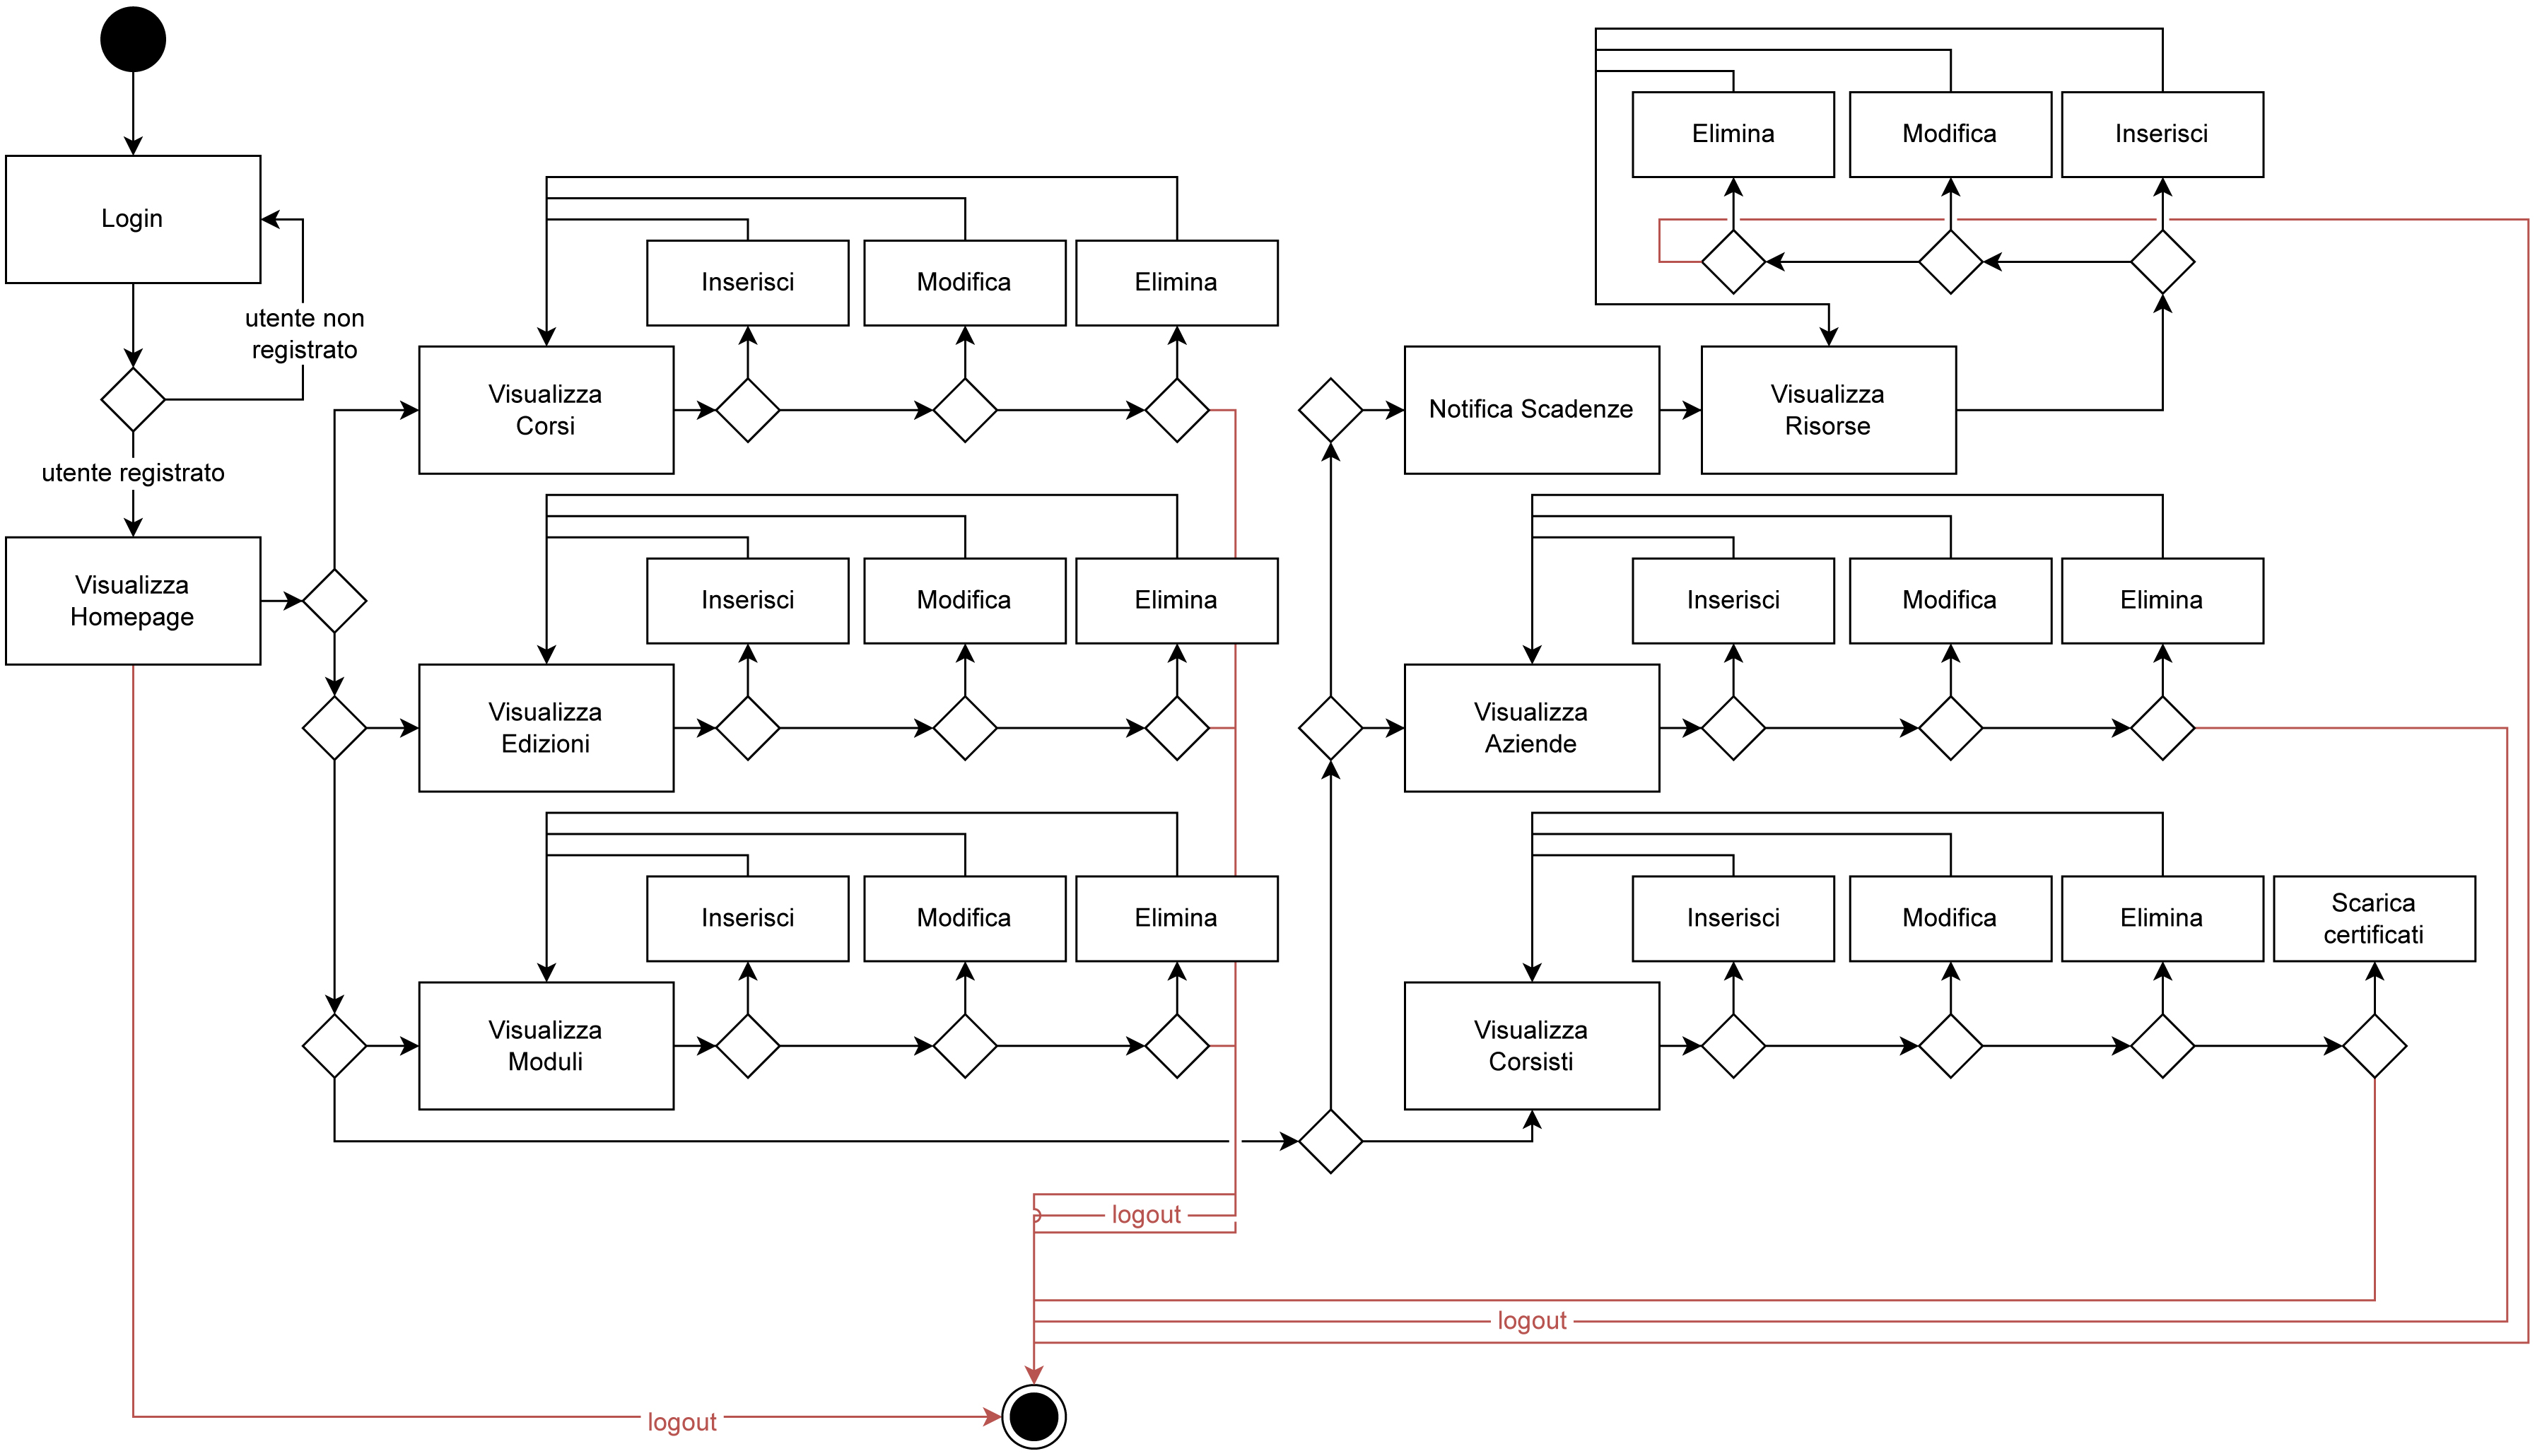
\includegraphics[scale=0.55]{img/Diagramma delle attivita.jpg}
\caption{Diagramma delle attività}
\label{fig:Diagrammadelleattivita}
\end{figure}
\noindent
Il diagramma in figura \ref{fig:Diagrammadelleattivita} rappresenta il diagramma delle attività per l'utente che opera con il sistema che, una volta autenticato, accede a tutte le funzionalità del gestionale.\\
Ogni rettangolo identifica un nodo del grafo o come azione (ad esempio \textit{Visualizza Corsi}) o come nodo di controllo (come \textit{Logout}); i rombi sono invece nodi di decisione per coprire tutti i possibili percorsi tra le attività.



\section{Analisi del contesto}
\label{sec:contesto}
L'analisi del contesto è quella fase in cui si prendono in considerazione le iterazione che il software ha con gli altri sistemi in relazione al flusso di informazioni.

\subsection{Diagramma di contesto}
\begin{figure}[h]
\centering
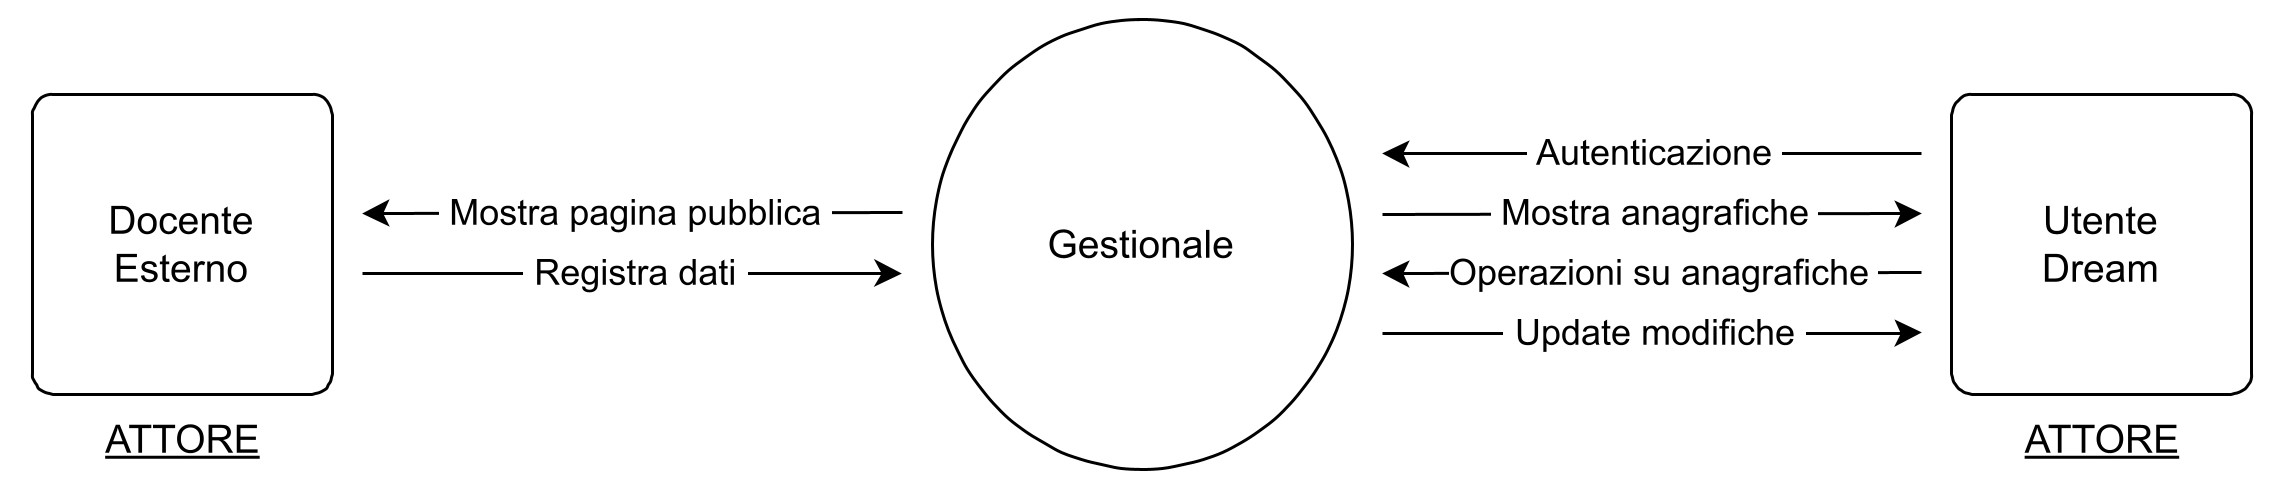
\includegraphics[scale=0.8]{img/Diagramma di Contesto.jpg}
\caption{Diagramma di contesto}
\label{fig:Diagrammadicontesto}
\end{figure}
\noindent
Il diagramma in figura \ref{fig:Diagrammadicontesto} rappresenta le interfacce esterne con cui il gestionale comunica. Si individuano due attori (entità che producono o consumano informazioni necessarie per l’elaborazione delle richieste): \textit{Utente Dream} e \textit{Docente Esterno}, il primo rappresenta l'utente che all'interno dell'azienda utilizza il gestionale mentre il secondo identica un docente che accede alla pagina pubblica per la registrazione a sistema dei suoi dati. Le frecce nel diagramma mostrano i flussi di informazioni.

\section{Analisi dei componenti}
\label{sec:componenti}
Questa fase di analisi ha l'obiettivo di modellare le connessioni tra i componenti, intesi come singoli moduli del software, in modo da evidenziare le relazioni tra essi e verificare che tutti i compiti che il sistema deve svolgere siano implementati. 
\subsection{Diagramma dei componenti}
\begin{figure}[h]
\centering
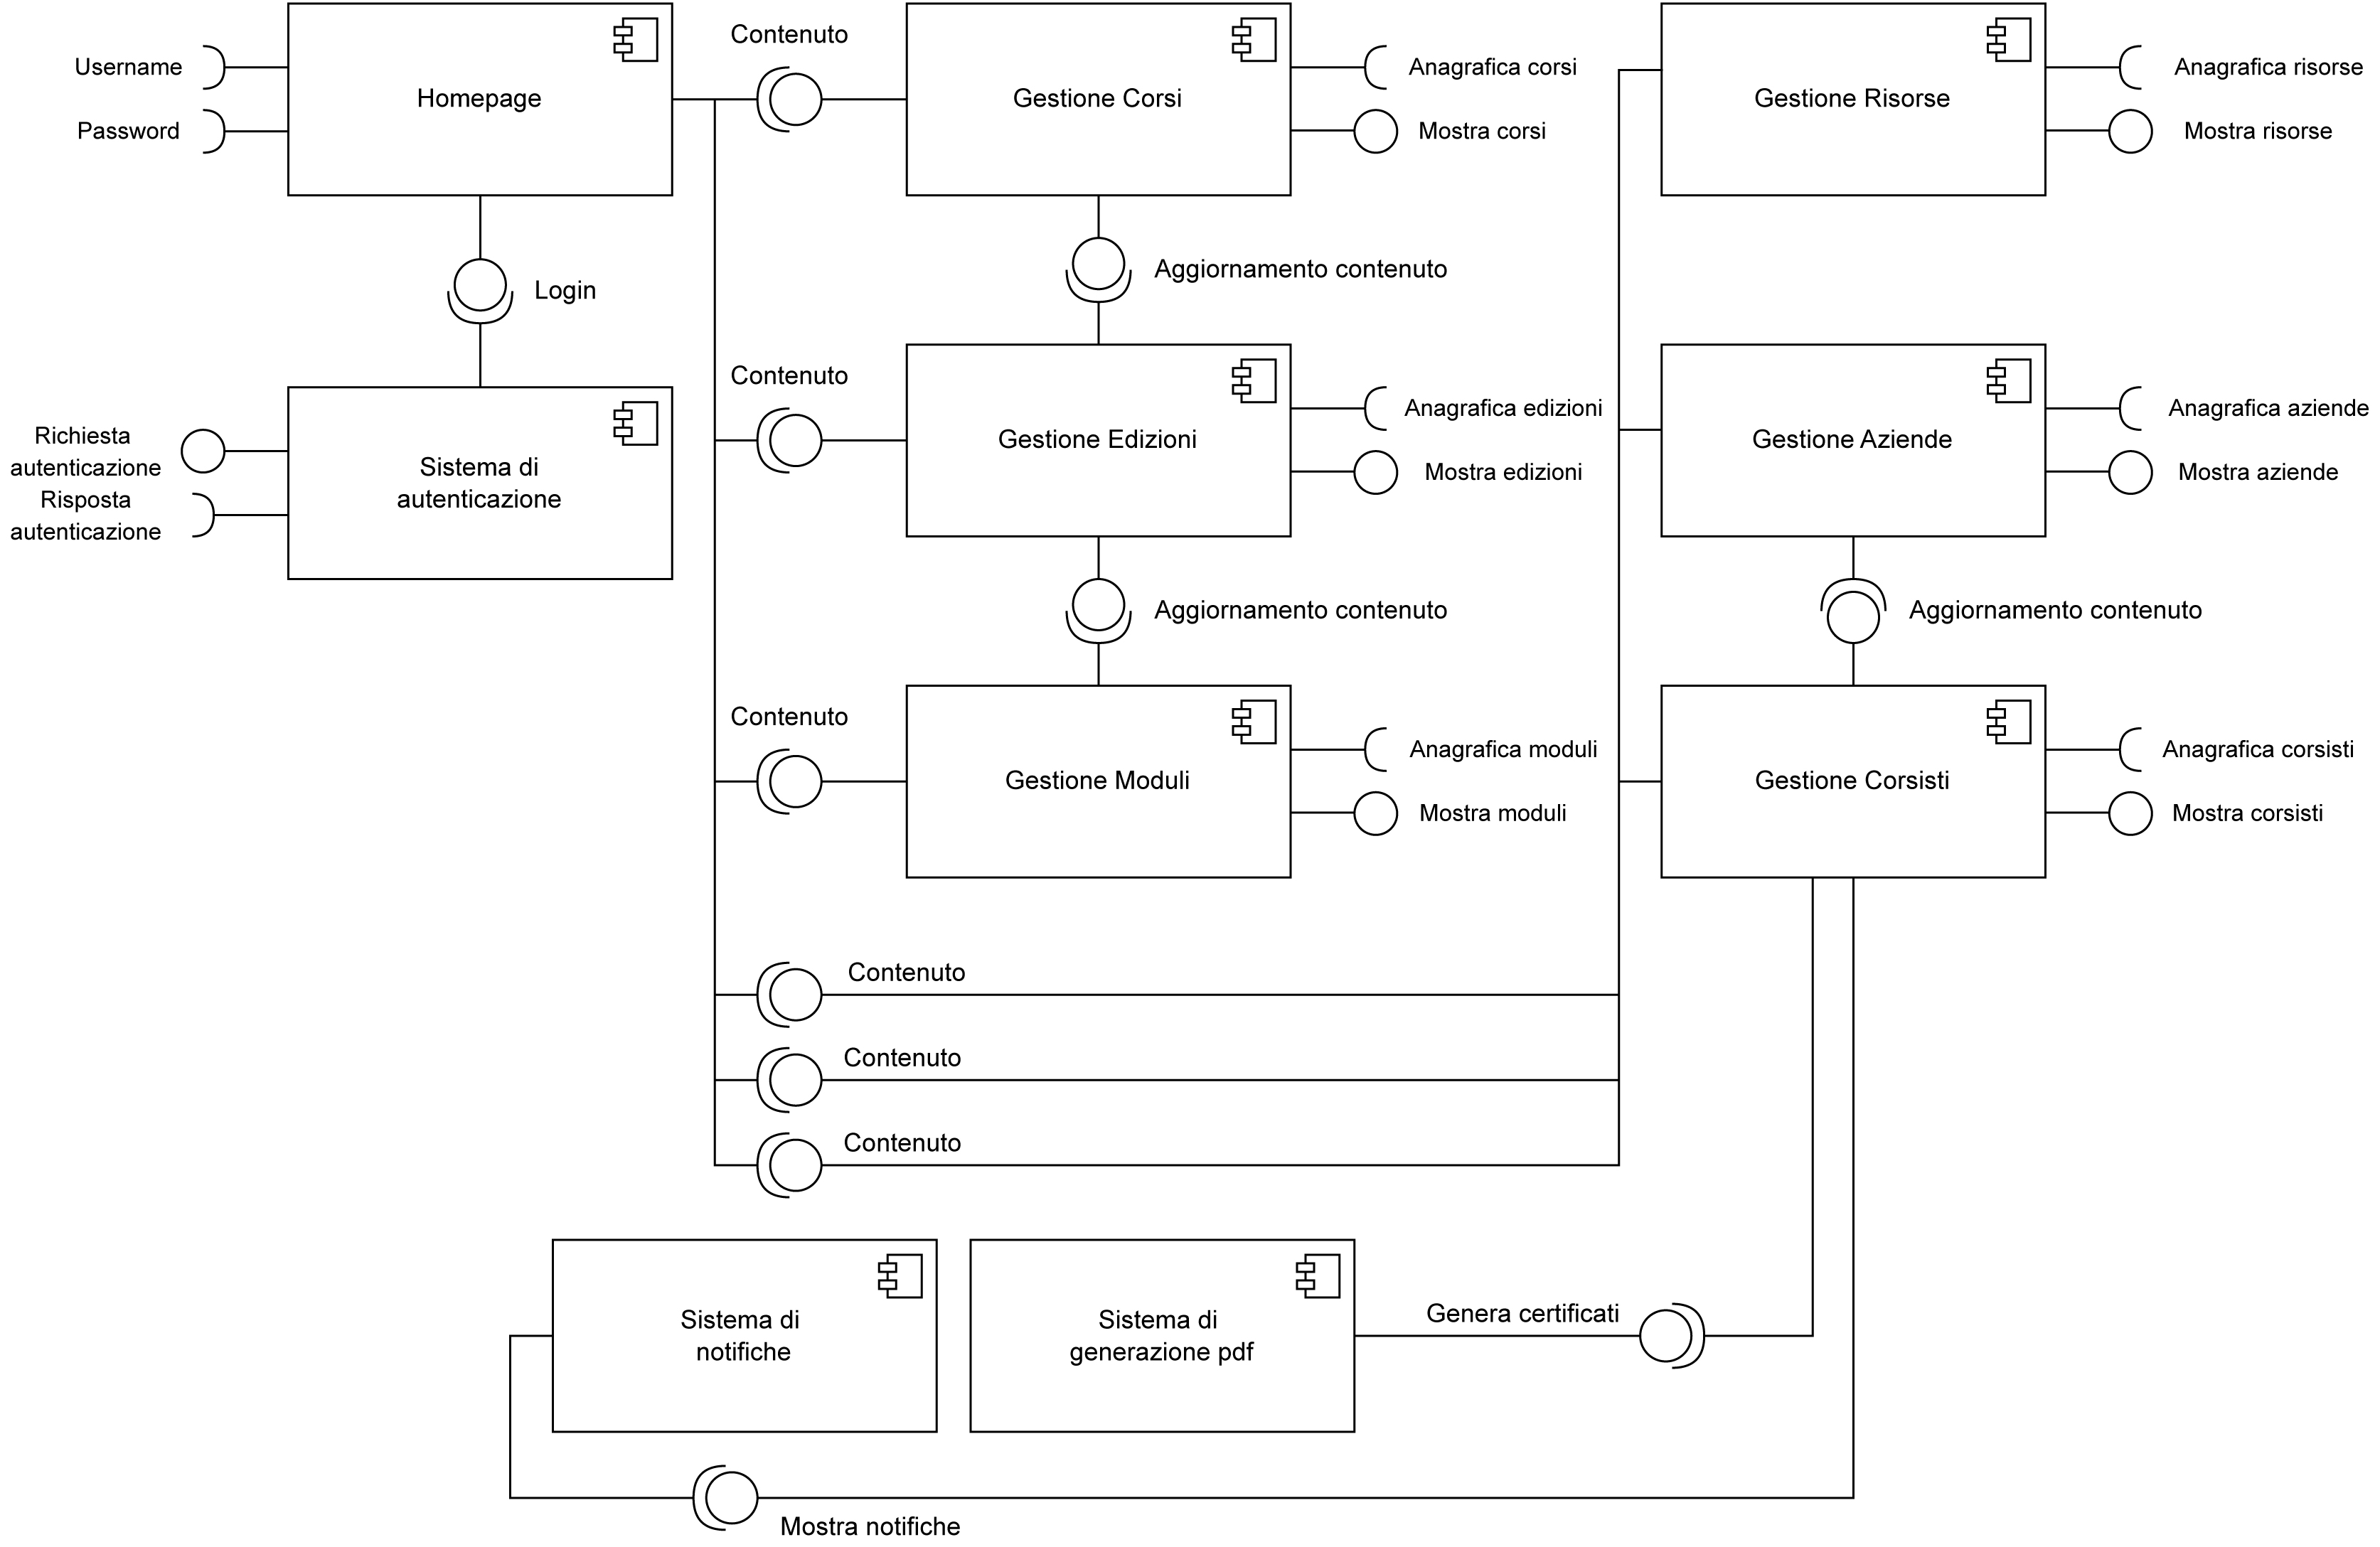
\includegraphics[scale=0.55]{img/Diagramma dei componenti.jpg}
\caption{Diagramma dei componenti}
\label{fig:Diagrammadeicomponenti}
\end{figure}
\noindent
In figura \ref{fig:Diagrammadicontesto} i rettangoli mappano i componenti mentre le relazioni tra due componenti individuano le interfacce. Le relazioni presentano un semicerchio se l'interfaccia è richiesta da un componente che ne consuma le informazioni, se, invece, sono rappresentate con un cerchio allora l'interfaccia in questione è messa a disposizione del componente che ne produce le informazioni. %temp

    \chapter{Ambito dell'elaborato e del progetto}
\label{cha:ambito}
Questo capitolo ha lo scopo di illustrare ad alto livello il lavoro svolto durante il tirocinio riguardante la progettazione e l'implementazione del software gestionale aziendale. In particolare si riportano, in modo più astratto, alcuni temi legati ai Sistemi Informativi \cite{SI} e alla gestione dei processi delle organizzazioni. I capitoli successivi, invece, entrano maggiormente nei dettagli di analisi e sviluppo tecnico.\newline
Di seguito si introducono argomenti relativi ai profili informativi, alla potenzialità e attrattività informatica e alla costruzione di un sistema informativo, presentando prima una breve spiegazione del tema e specificando poi il posizionamento del documento rispetto al concetto espresso.   

\subsection{L'esigenza informativa}
\label{sec:anthony}
Il ruolo principale di ogni sistema informativo è quello di fornire aiuto e supporto alla gestione aziendale aumentando il livello di astrazione con l'aumentare del livello decisionale.
Le operazioni svolte possono essere classificate in base alle attività compiute e ai requisiti richiesti dai vari attori che lavorano dell'organizzazione. Per rappresentare questa divisione si fa spesso riferimento alla Piramide di Anthony \cite{anthony}\cite{anthony2} (figura \ref{fig:anthony}), schema composto da tre livelli, ognuno dei quali svolge incarichi differenti e possiede un profilo informativo diverso assegnato. Il livello base riguarda infatti il personale esecutivo con attività operative, la parte intermedia dello schema coinvolge la direzione funzionale con attività tattiche, mentre la punta della piramide riguarda i processi dell'alta direzione con i ruoli più strategici.
\begin{figure}[!hbt]
\centering
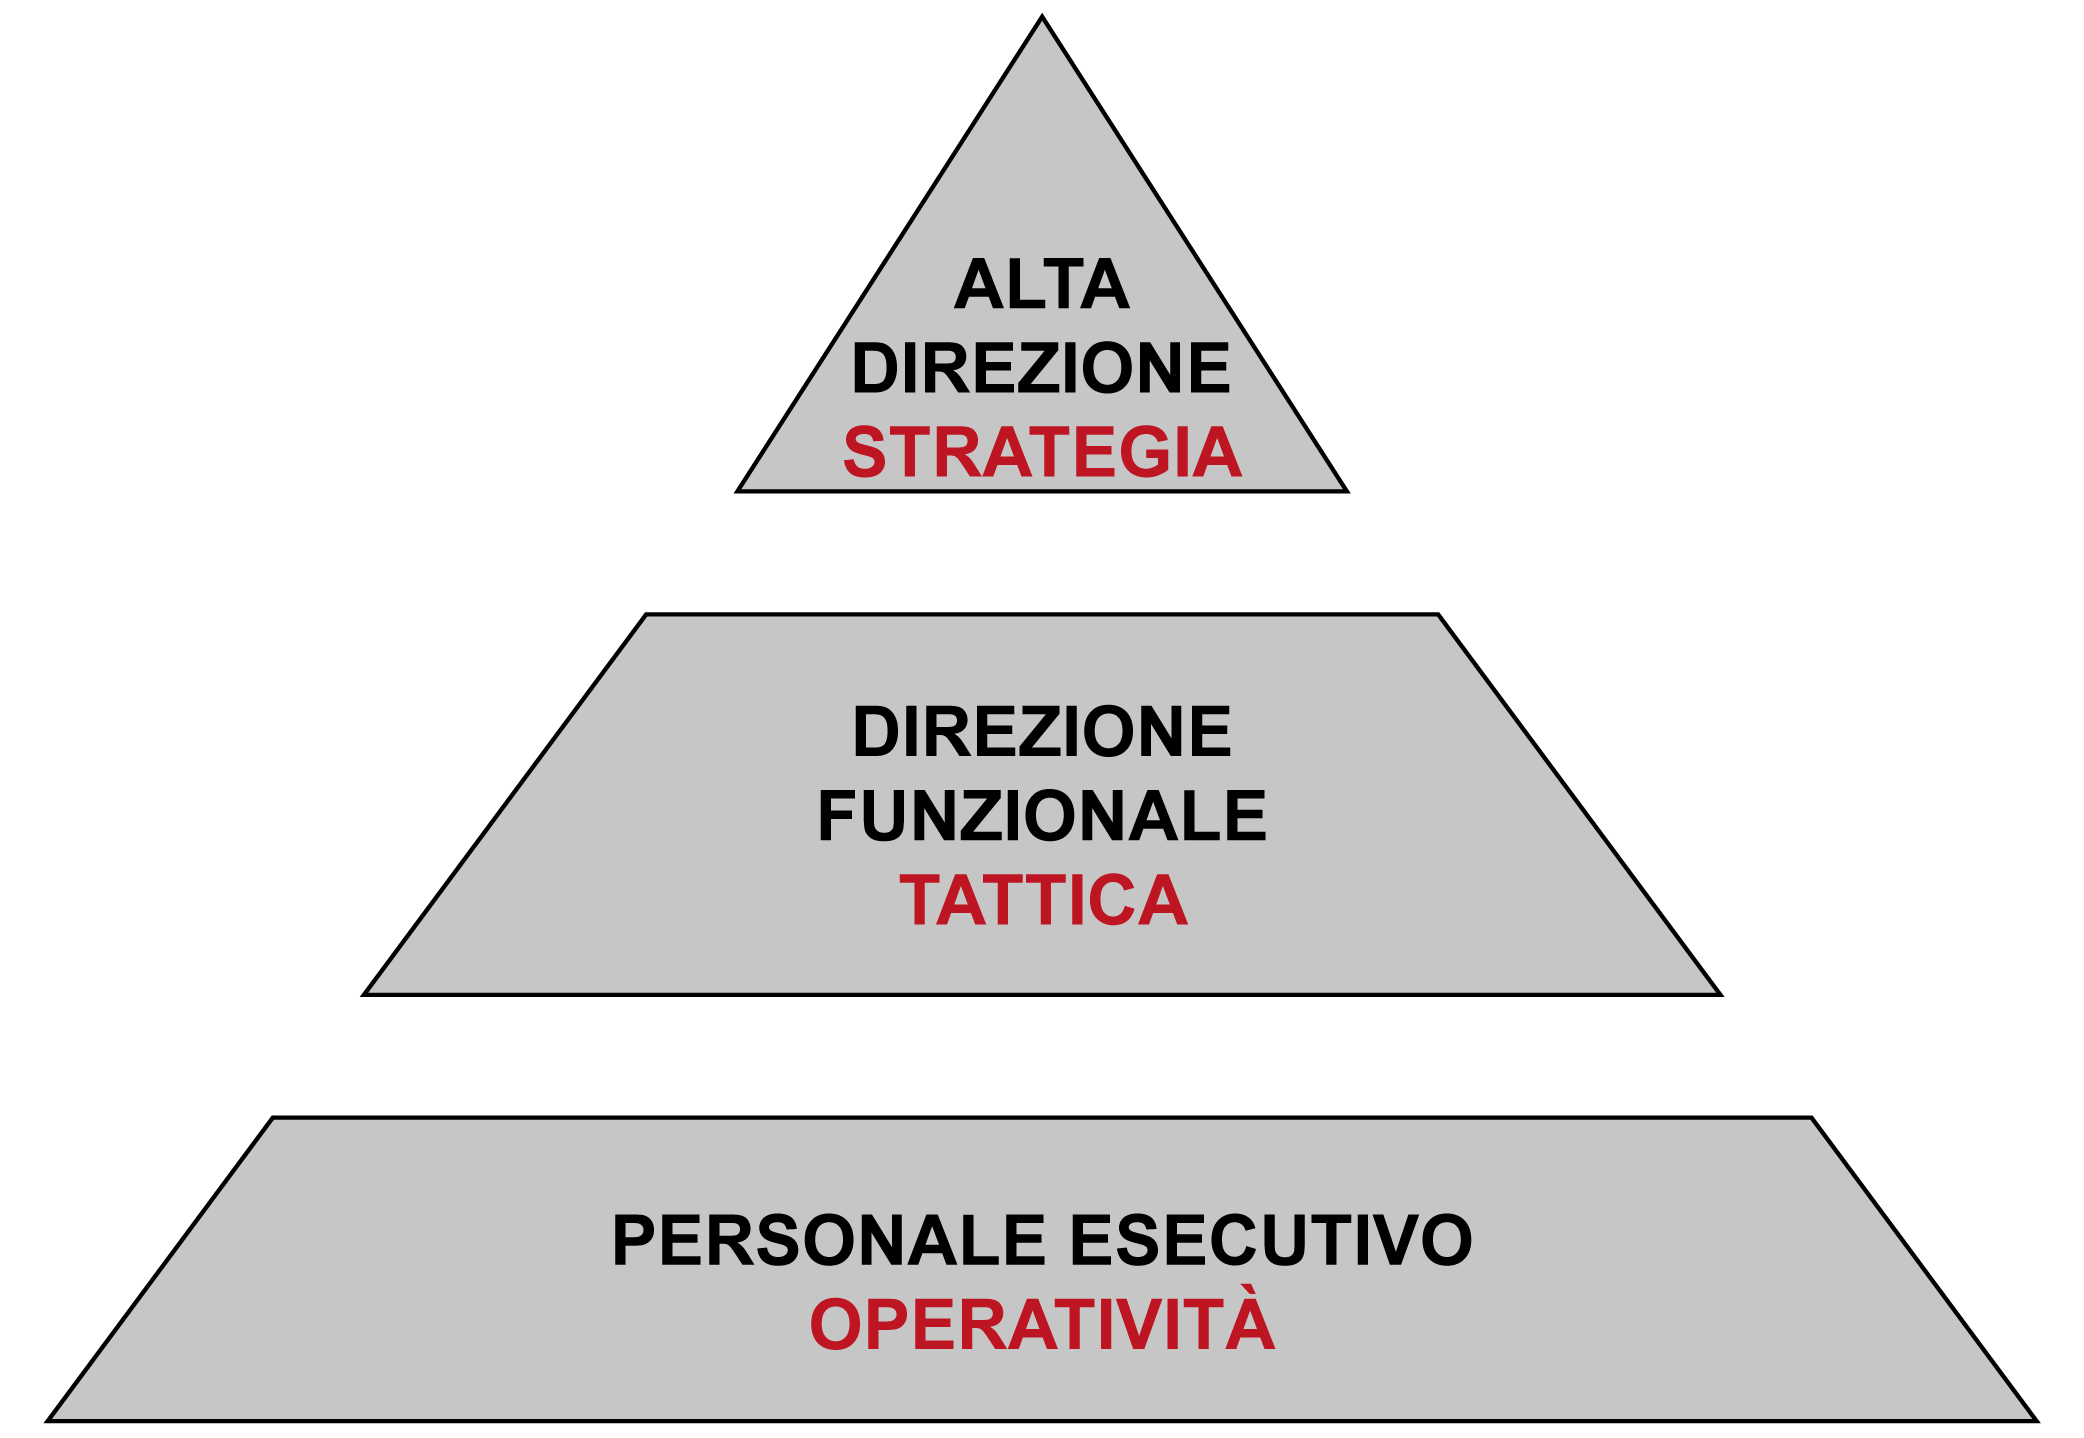
\includegraphics[scale=0.45]{img/anthony_scheme.png}
\caption{Piramide di Anthony}
\label{fig:anthony}
\end{figure}
\newline
\noindent
I processi trattati e analizzati nel progetto seguito si collocano a livello operativo che lavora con grandi volumi di dati precisi, analitici e interni all'azienda, con frequenza continua. Queste attività richiedono informazioni dettagliate ed esatte, fornite con tempestività; raramente si opera con dati sintetici. \\
\newline
Per quanto riguarda la scomposizione del sistema informativo, la collocazione dei processi implementati ricade sul sistema operazionale (e non su quello informazionale). Le funzioni principali sono perciò quelle di aiutare l'azienda nell'automatizzare tutte le operazioni procedurali dell'area coinvolta, definire e integrare nuovi processi e rendere guidate e strutturate le attività esecutive. L'obiettivo è pertanto quello di permettere l'accesso alle informazioni attuali in modo interattivo, con la possibilità di leggere, modificare ed inserire nuovi dati. Questi tipi di sistemi usano un database operazionale \cite{operational_database} e una serie di metodi operativi per rendere possibile un'analisi OLTP (On Line Transaction Processing) \cite{oltp}. L'elaborazione dei dati prevede l'esecuzione di molte transizioni contemporanee di vari utenti che accedono alla base di dati effettuando ricerche e/o modifiche, e garantisce in qualsiasi momento l'accesso alle informazioni in modo coerente e corretto.

\subsection{L'attrattività informatica}
\label{sec:attrattivita}
I sistemi operazionali hanno come obiettivo principale quello di permettere la pianificazione e il controllo dei processi coinvolti, con conseguente acquisizione e organizzazione della conoscenza e delle situazioni dell'impresa. Per questo motivo è spesso utile definire quella che viene considerata la ``potenzialità informatica'' di un'azienda. Questo concetto viene influenzato da vari fattori come la propensione all'uso e all'implementazione di strutture tecnologiche e informatiche a sostegno delle attività, l'intensità informativa (definito dalla struttura dell'organizzazione e dalla quantità di informazioni necessarie) e l'attrattività informatica.
Quest'ultimo parametro è legato al grado di efficacia, facilità e competenza nel rendere informatizzato un processo aziendale.\\
\begin{figure}[!hbt]
\centering
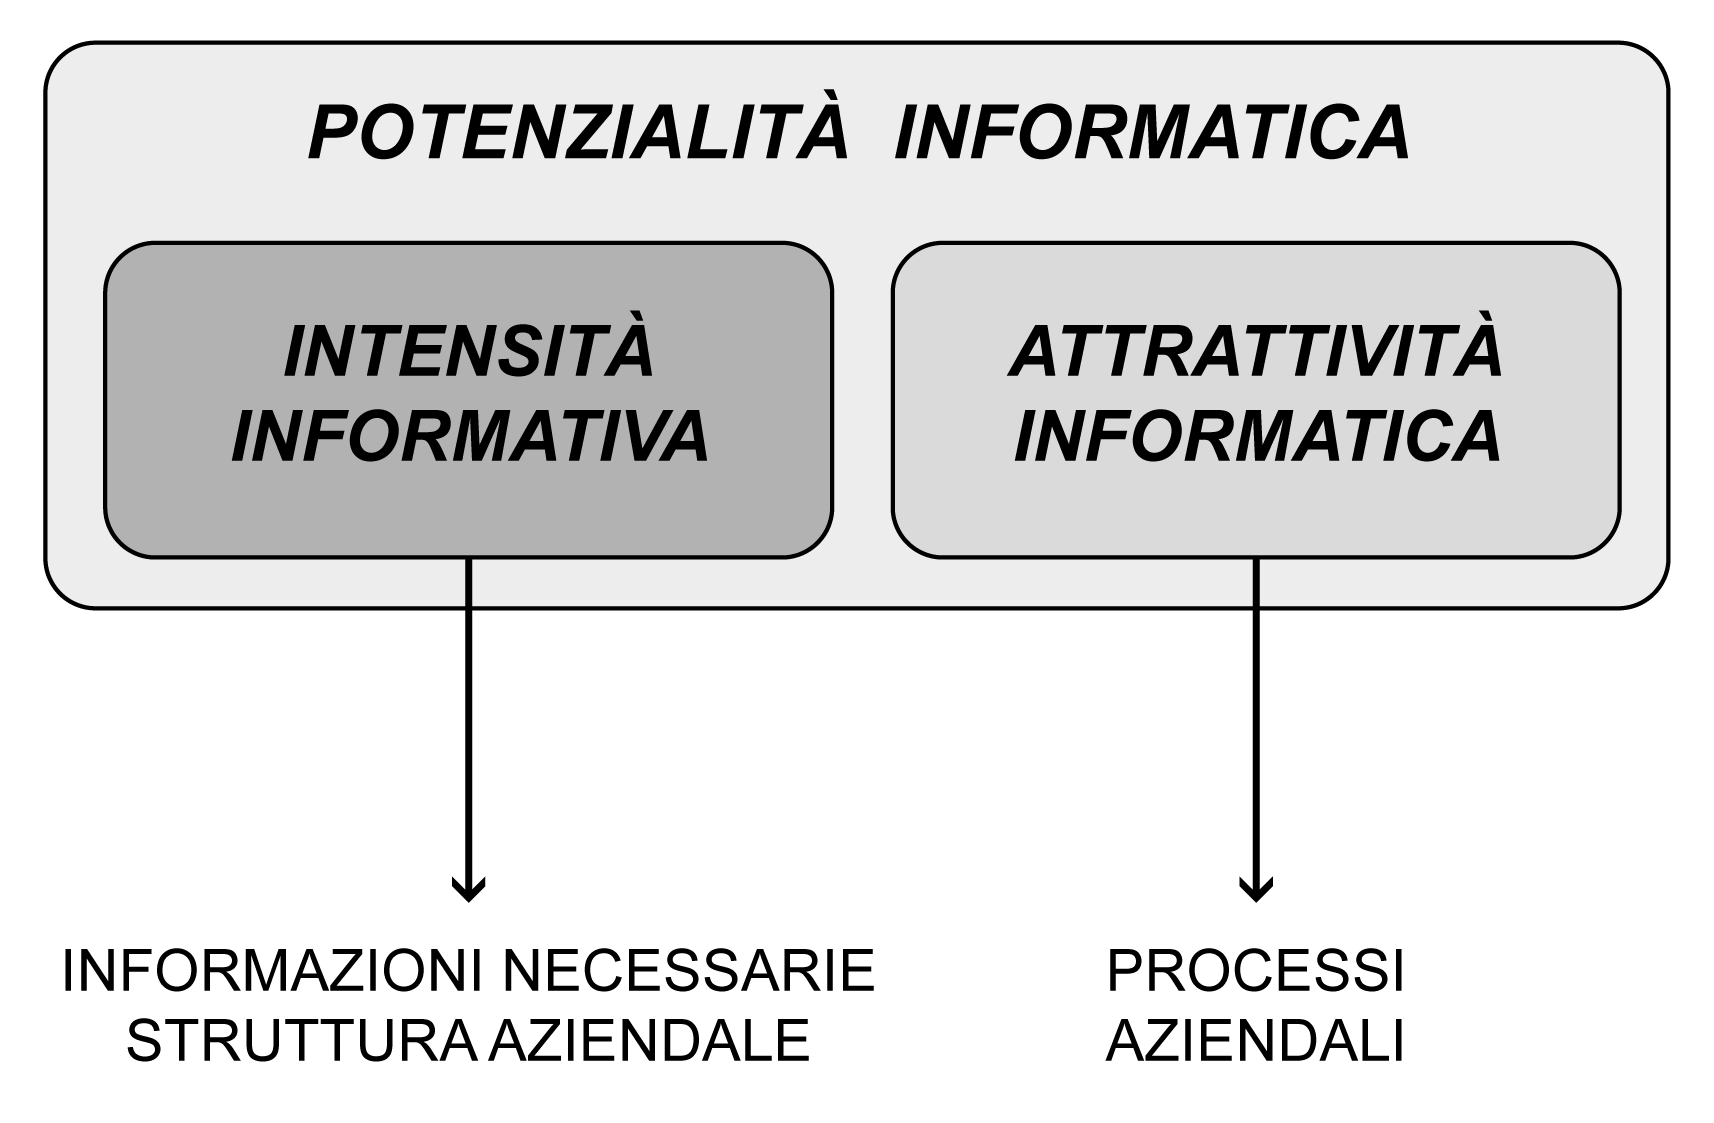
\includegraphics[scale=0.55]{img/potenzialita.png}
\caption{Potenzialità Informatica}
\label{fig:potenzialita}
\end{figure}
\noindent
\newline
La necessità di sviluppare il gestionale richiesto è stata ponderata in base proprio all'elevata attrattività informatica di tutti i processi coinvolti in questo progetto. Questa esigenza è stata determinata dall'elevato grado procedurale, ovvero di strutturazione dei flussi coinvolti e dall'alta ripetitività, intesa come la frequenza di ripetizione nel tempo di una sequenza di operazioni senza particolari modifiche. Inoltre, dati gli elevati volumi di informazioni da elaborare e il basso o medio grado di difficoltà di molte azioni elementari del processo, è evidente l'elevata attrattiva informatica dell'intero applicativo richiesto; a questo si aggiungono anche la buona propensione e le abitudini delle figure interne all'azienda nell'usare già sistemi informatici per altri processi.      
\begin{figure}[!hbt]
\centering
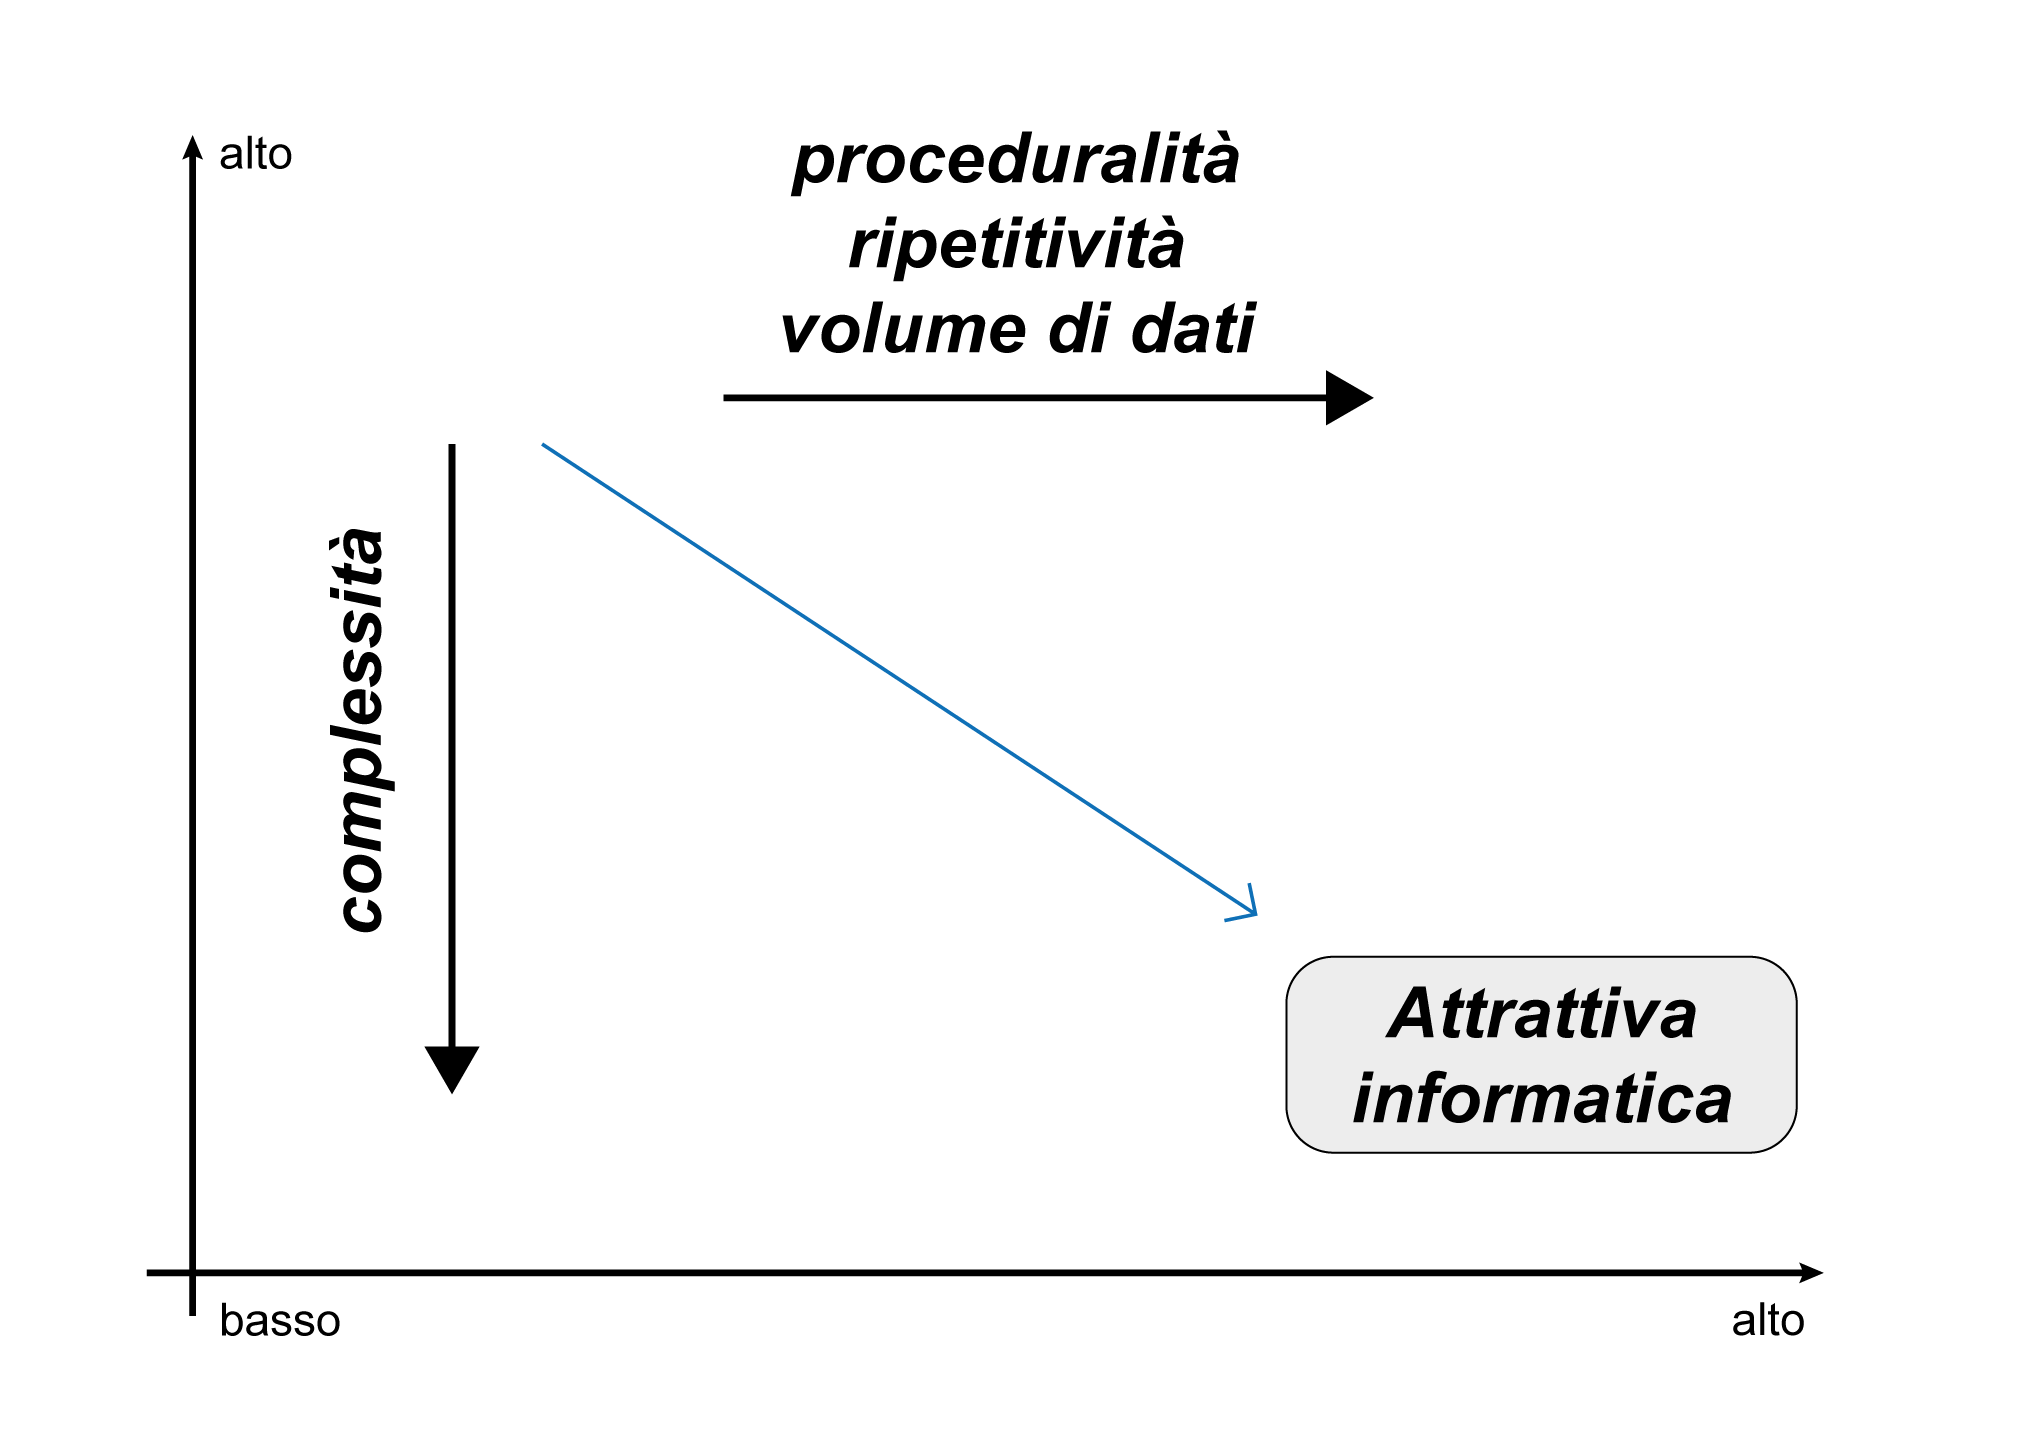
\includegraphics[scale=0.55]{img/attrattiva.png}
\caption{Attrattiva Informatica}
\label{fig:attrattiva}
\end{figure}
\noindent
\newline


\subsection{Costruzione del Sistema Informativo}
\label{sec:make}
Durante la fase di digitalizzazione dei processi e, quindi, di costruzione del Sistema Informativo, ogni azienda è tenuta a prendere una decisione in termini di possibili percorsi da seguire, scegliendo tra:
\begin{itemize}
    \item \textit{Make}
    \item \textit{Buy}
    \item \textit{Outsource}
\end{itemize}
La prima opzione consiste, in sintesi, nel costruire tutti gli applicativi e servizi del Sistema Informativo in modo interno e autonomo, presupponendo la presenza di un gruppo di lavoro in grado non solo di progettare il sistema nel presente, ma anche di mantenerlo nel tempo. La scelta di acquisto invece prevede di comprare il software da fornitori esterni; è la scelta più comune nelle piccole e medie imprese in quanto richiede solo di avere delle figure per gestire gli utenti interni e comunicare con i tecnici distributori. Nonostante la maggior flessibilità rispetto all'opzione \textit{Make} e il vantaggio in termini di confronto con il mercato, l'organizzazione è totalmente dipendente da una struttura esterna. L'ultima possibilità è quella di affidare la gestione e l'organizzazione del Sistema Informativo a un ente  esterno; questa scelta sta diventando sempre più popolare in quanto, a fronte di un canone periodico, costi più bassi, garanzie di sicurezza e di connettività si uniscono alla flessibilità interna e ai vantaggi del \textit{Buy}. Si deve però accettare la perdita di controllo su un elemento molto importante del modello organizzativo aziendale.
\begin{figure}[!hbt]
\centering
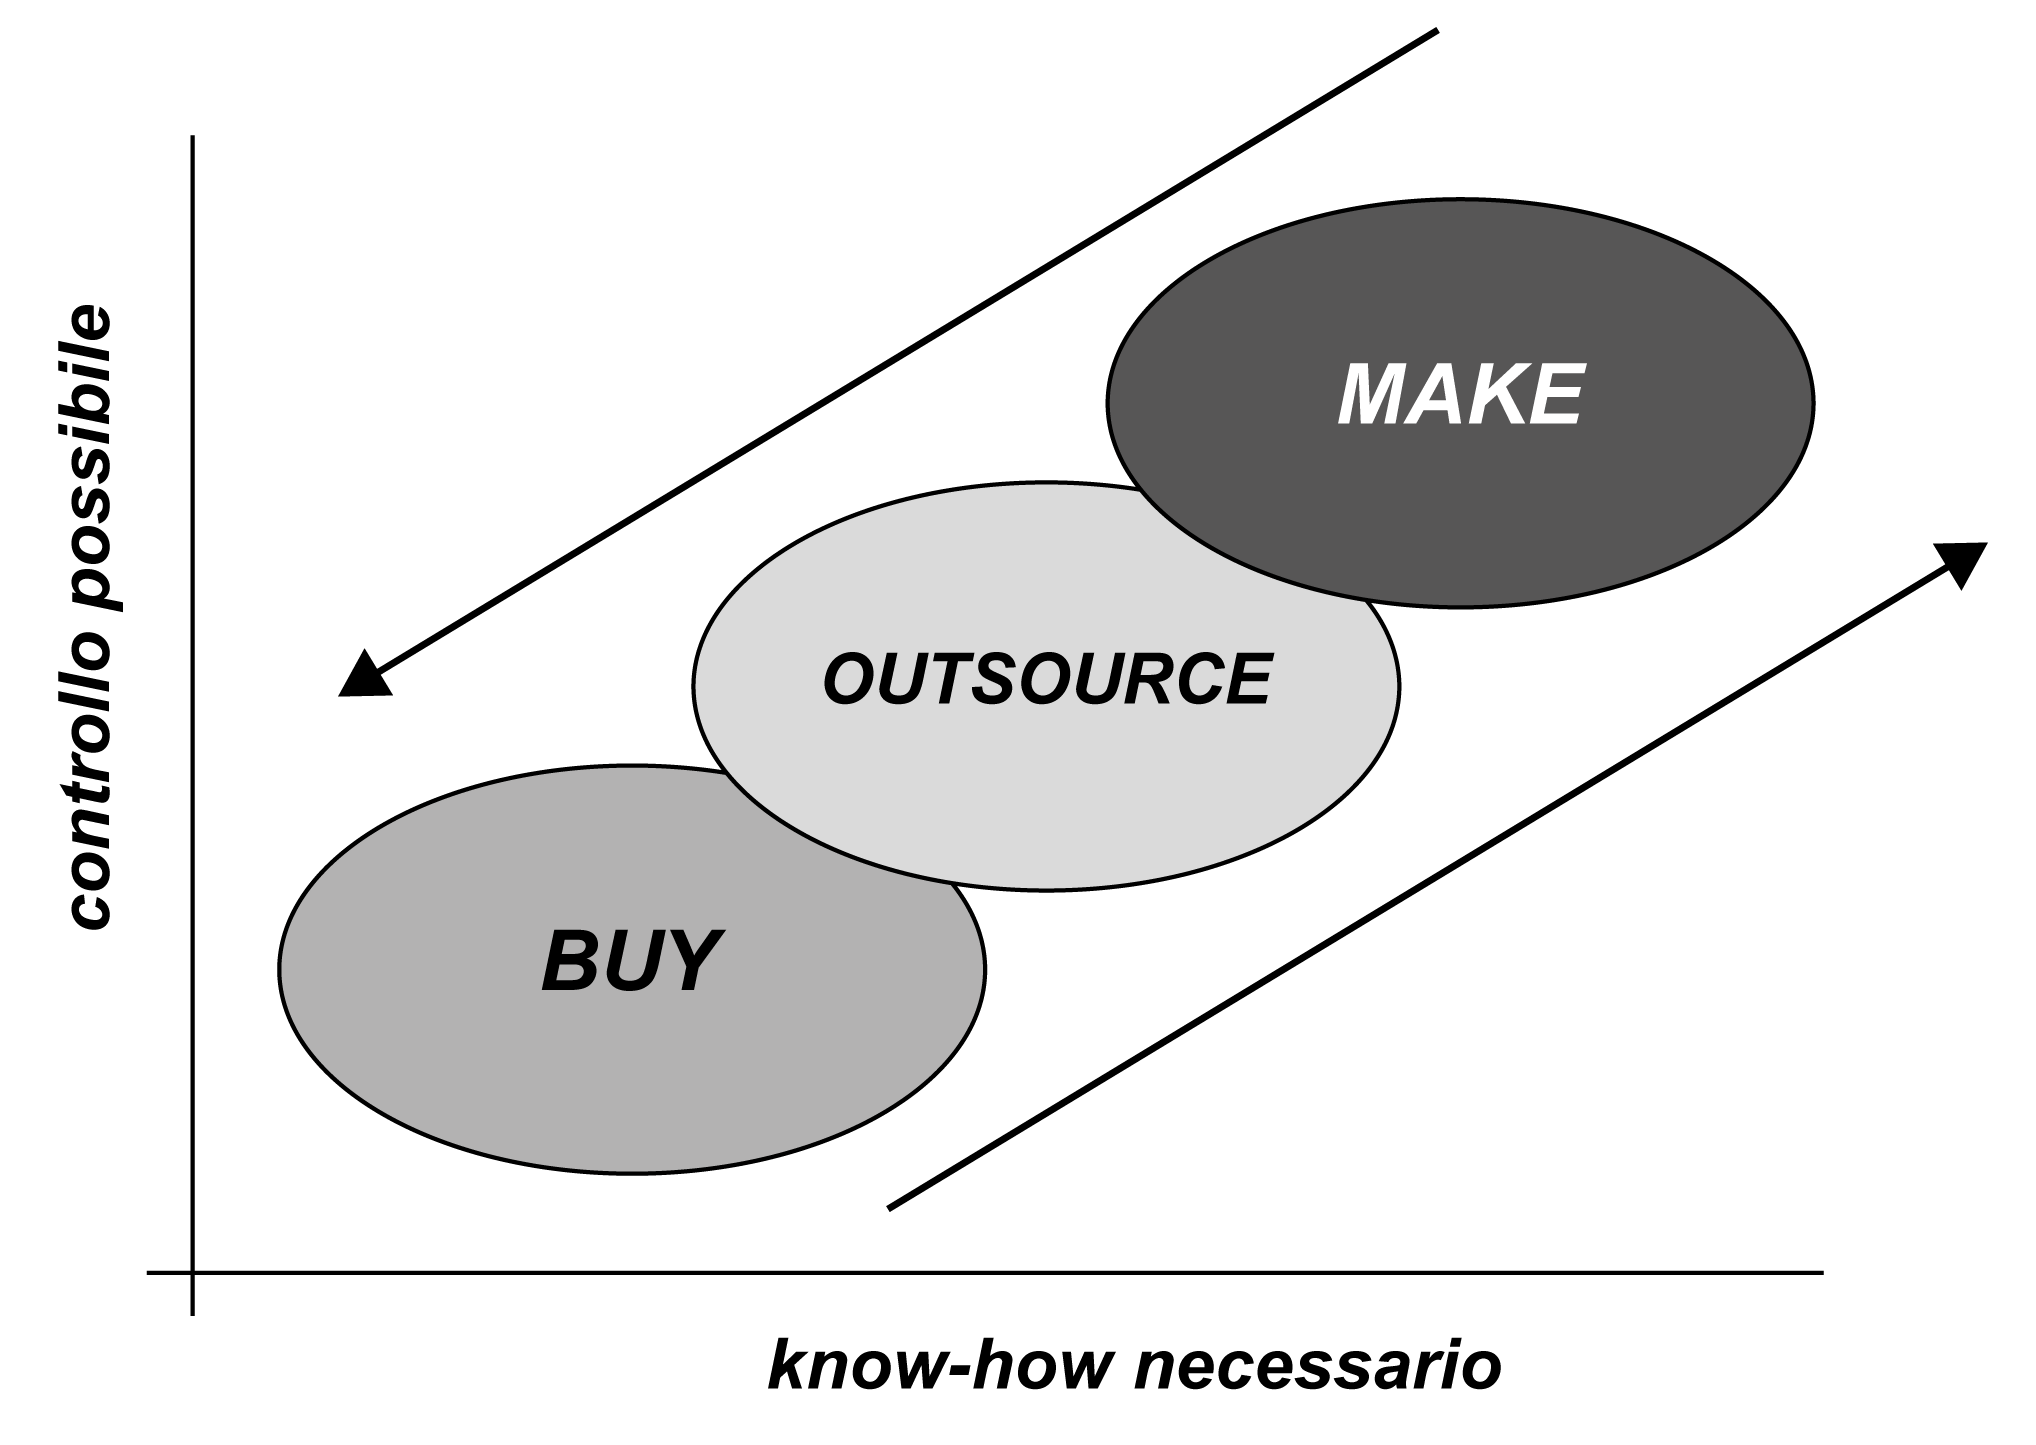
\includegraphics[scale=0.55]{img/makevsbuy.png}
\caption{Costruzione del SI: le possibilità}
\label{fig:makevsbuy}
\end{figure}
\newline
\noindent
Una volta individuati, se pur ad alto livello, i processi interessati da automatizzare, nella prima fase del tirocinio si sono analizzati con precisione tutti i vantaggi e le conseguenze di ognuna delle opzioni disponibili elencate per l'implementazione del software richiesto. Dopo una primo periodo di ricerca sul mercato di possibili soluzioni acquistabili che rispettassero i requisiti stabiliti, si è arrivati alla conclusione di scegliere l'approccio \textit{Make} per ottenere una mappatura puntuale e su misura del modello organizzativo in questione. Si è infatti considerata la complessità relativamente contenuta, almeno per una prima versione base del gestionale, e la necessità di avere un'automatizzazione dei flussi di lavoro per lo più personalizzati e ``ad hoc''. La soluzione di produrre interamente un applicativo o un servizio rappresenta, per la maggior parte delle PMI, una scelta non comune, dati gli investimenti necessari generalmente elevati e la mancanza di inserimento e confronto con il mercato. Al contrario, in questo specifico caso, è risultato vantaggioso creare il gestionale internamente grazie ai costi pressoché nulli e al know-how aziendale già presente.              
\clearpage
\newpage
      \chapter{Analisi dei requisiti}
\label{cha:intro}

L'analisi dei requisiti o l'ingegneria dei requisiti è il processo usato per determinare le esigenze e le aspettative degli utenti verso un nuovo prodotto.
Lo scopo di questo tipo di analisi è di trasformare le richieste delle parti interessate e degli utenti finali, raccolte ad alto livello, in specifiche misurabili, verificabili, coerenti e ben dettagliate \cite{req1}\cite{req2}\cite{req3}.



\section{Caso studio}
\label{sec:studio}
I casi studio più rilevanti sono quelli legati alla gestione delle varie anagrafiche, dalla visualizzazione, creazione, modifica ed eliminazione, all'utilizzo di funzioni operative più complesse su di esse.\\
Il flusso delle anagrafiche del progetto è così strutturato: un \textit{Corso} è formato da più \textit{Edizioni}, ognuna delle quali composta da vari \textit{Moduli}. Per \textit{Corsista} si intende un partecipante a uno o più moduli di un'edizione che può ottenere un \textit{Attestato} di frequenza. Ogni corsista può essere associato a un'\textit{Azienda}. Per \textit{Risorse} si identificano quelle persone che prendono parte a un corso con una funzione specifica; è quindi presente un'anagrafica completa di queste figure che permette anche la gestione di file PDF associati (come curriculum vitae o moduli privacy) e implementa un sistema di notifiche interne legate alle scadenze di questi documenti. L'ultima entità riguarda i \textit{Ruoli} che queste risorse possono avere sui moduli (docente, tutor, coordinatore, ecc.).




\section{Requisiti funzionali}
\label{sec:funzionali}
I requisiti funzionali definiscono le funzioni del sistema, ovvero ciò che questo deve fare in termini di interazione tra l'applicativo e il suo ambiente, indipendentemente dall'implementazione. Questo tipo di richieste può essere rappresentato dai casi d'uso, sequenza di azioni che producono un risultato osservabile da un attore, esplicitando cosa ci si aspetta dal sistema, ma nascondendone il comportamento.\\
Di seguito si riporta l'elenco dei principali requisiti funzionali individuati con una breve descrizione. Si nota che l'analisi relativa alle anagrafiche è riportata ad alto livello raggruppandole sotto un unico componente.
\subsection{Accesso protetto al sistema}
\textbf{Riassunto}: si descrive come avviene l'autenticazione di un utente che vuole accedere al gestionale.\\
\textbf{Descrizione:}
\begin{enumerate}
  \item L'utente non autenticato inserisce username e password per accedere.
  \item Il sistema verifica la correttezza dei dati inseriti interrogando il database.
  \item Se l'interrogazione ha esisto positivo l'utente autenticato accede alla homepage, altrimenti il sistema segnala la non correttezza dei dati.
\end{enumerate}

\subsection{Visualizzazione delle anagrafiche}
\textbf{Riassunto}: si descrive come il sistema mostra i dati relativi alle varie anagrafiche.\\
\textbf{Descrizione:}
\begin{enumerate}
  \item Il sistema presenta i dati dell'anagrafica selezionata in forma tabellare e strutturata.
  \item L'utente naviga nella tabella con la possibilità di filtrare o esplorare i dati.
  \item Il sistema risponde alle richieste dell'utente adattando la visualizzazione di conseguenza.
\end{enumerate}

\subsection{Memorizzazione delle anagrafiche}
\textbf{Riassunto}: si descrive come il sistema garantisce la memorizzazione di nuovi dati relativi alle anagrafiche.\\
\textbf{Descrizione:}
\begin{enumerate}
  \item L'utente aggiunge nuovi elementi alle anagrafiche inserendo i dati richiesti dal sistema.
  \item Il sistema verifica la correttezza e la completezza dei dati inseriti. Se la verifica ha esito positivo prosegue altrimenti segnala l'errore.
  \item Il sistema memorizza nel database il nuovo elemento.
  \item Il sistema aggiorna la visualizzazione dei dati.
\end{enumerate}

\subsection{Gestione delle anagrafiche}
\textbf{Riassunto}: si descrive come l'utente accede alle funzionalità dei dati relativi alle anagrafiche.\\
\textbf{Descrizione:}
\begin{enumerate}
  \item L'utente seleziona un elemento di un'anagrafica.
  \item Se l'utente sceglie di modificare un elemento:
  \begin{enumerate}
    \item Il sistema verifica la correttezza e la completezza dei nuovi dati. Se la verifica ha esito positivo prosegue altrimenti segnala l'errore.
    \item Il sistema aggiorna l'elemento nel database.
    \item Il sistema aggiorna la visualizzazione dei dati.
  \end{enumerate}
  \item Se l'utente sceglie di eliminare un elemento:
  \begin{enumerate}
    \item Il sistema verifica la possibilità di eliminare l'elemento in termini di non violazione di vincoli con altri elementi. Se la verifica ha esito positivo prosegue altrimenti segnala l'errore.
    \item Il sistema elimina l'elemento dal database.
    \item Il sistema aggiorna la visualizzazione dei dati.
  \end{enumerate}
\end{enumerate}

\subsection{Logout dal sistema}
\textbf{Riassunto}: si descrive come l'utente esce dal sistema.\\
\textbf{Descrizione:}
\begin{enumerate}
  \item L'utente autenticato effettua il logout.
  \item Il sistema termina la sessione dell'utente, che viene scollegato.
\end{enumerate}



\section{Requisiti non funzionali}
\label{sec:nonfunzionali}
I requisiti non funzionali rappresentano i vincoli che il sistema deve soddisfare nella sua totalità. Queste richieste non sono legate a singole funzioni fornite dal software, ma a caratteristiche che questo deve avere in termini di qualità del sistema o vincoli a cui deve sottostare.\\
Di seguito di riporta un elenco dei principali requisiti non funzionali raccolti, con una breve descrizione corrispondente.

\subsection{Responsive web design}
L'applicativo deve essere in grado di adattarsi graficamente in maniera automatica e fluida a qualsiasi dispositivo utilizzato. Il gestionale riconosce quindi il dispositivo utilizzato dall’utente e adatta il suo layout alle specifiche dimensioni del display.

\subsection{Sicurezza}
Il sistema protegge il suo contenuto da accessi non autorizzati e prevede delle norme di sicurezza in termini di:
\begin{itemize}
  \item Conferma di identità: all'utente non autenticato viene mostrata la pagina di login e solo dopo il corretto inserimento dei dati, con verifica tramite interrogazione al database, potrà accedere al gestionale. 
  \item Sicurezza di trasmissione dei dati: il sistema adotta le tecniche per garantire la riservatezza, l'integrità e la disponibilità dei dati trasmessi ed elaborati, anche e soprattutto tramite l'utilizzo del protocollo \texttt{https} \cite{https}.
  \item Sicurezza delle password: la memorizzazione delle password nel database avviene in maniera criptata; la creazione di una nuova password per l'utente prevede dei vincoli di robustezza e sicurezza quali: lunghezza di almeno 10 caratteri, presenza di almeno 2 lettere maiuscole, 2 simboli e 4 numeri.
\end{itemize}

\subsection{Affidabilità}
Il sistema deve rispettare le specifiche tecniche di funzionamento nel tempo \cite{affidabilita}.
Per far fronte a tale requisito sono stati imposti dei vincoli di affidabilità:

\begin{table}[h!]
\centering
\begin{tabular}{|l|l|l|}
\hline
\multicolumn{1}{|c|}{\textbf{Vincolo}} & \multicolumn{1}{c|}{\textbf{Descrizione}} & \multicolumn{1}{c|}{\textbf{Misura}} \\ \hline
Tempo di attesa                        & Tempo massimo di risposta alla richiesta  & ≤ 1,5 secondi                        \\ \hline
Tasso di fallimento                    & Risposta a ogni richiesta inviata         & ≤ 0,5\%                              \\ \hline
Tentativo di recupero                  & Riprovare la richiesta fallita            & 5 volte a intervalli di 2 secondi    \\ \hline
\end{tabular}
\caption{Tabella dei vincoli di affidabilità.}
\label{}
\end{table}

\subsection{Usabilità}
Gli utenti devono essere in grado di navigare tra le risorse e portare a termine le operazioni previste in modo facile e chiaro. Il sistema deve quindi essere semplice da usare ed efficiente nella sua integrità. 

\subsection{Prestazioni}
Il gestionale deve essere veloce in fase di avvio e fluido durante la transizione da una pagina all'altra, nel caricamento, nella visualizzazione dei dati, e nello svolgimento di ogni operazione.
Per garantire tale requisito sono stati imposti dei vincoli di performance:
\begin{table}[h!]
\centering
\begin{tabular}{|l|l|l|}
\hline
\multicolumn{1}{|c|}{\textbf{Vincolo}} & \multicolumn{1}{c|}{\textbf{Misura}} \\ \hline
Avvio della pagina principale &  Entro 1 secondo\\ \hline
Transizione tra pagine & Entro 1 secondo\\ \hline
Caricamento dei dati & Entro 3 secondi\\ \hline
Operazione sui dati & Entro 3 secondi\\ \hline
\end{tabular}
\caption{Tabella dei vincoli di performance.}
\label{}
\end{table}
\noindent
\newline
Il sistema deve inoltre gestire l'accesso contemporaneo di più utenti senza alcun degrado delle prestazioni.

\subsection{Scalabilità}
Il sistema riesce a gestire un numero crescente di utenti che accede al gestionale in simultanea e processa i dati prodotti dagli utenti stessi.     
L'applicativo deve essere anche in grado di aumentare o diminuire in termini di utenti e dati contenuti in base alle esigenze.

\subsection{Compatibilità e Portabilità}
Il software non necessita di installazione all'interno del sistema operativo su cui viene eseguito; la sua compatibilità e portabilità sono strettamente legate al browser utilizzato. Il sistema deve perciò essere utilizzabile attraverso i browser più popolari \cite{browsers} come:
\begin{itemize}
  \item Google Chrome, dalla versione 3.22.24.10 \cite{chrome}.
  \item Mozilla Firefox, dalla versione 27 \cite{firefox}.
  \item Safari, dalla versione 8.0 \cite{safari}.
  \item Microsoft Edge, dalla versione 0.11.10051 \cite{edge}.
\end{itemize}
e altri.



\subsection{Manutenzione}
Dopo il rilascio del sistema deve essere possibile in modo semplice ed efficace eliminare malfunzionamenti, migliorare le prestazioni, e inserire nuove funzionalità con aggiornamenti.

\section{Analisi delle attività}
\label{sec:contesto}
La fase di analisi delle attività ha come obiettivo la modellazione del flusso di lavoro dell'intero sistema che viene visto come un insieme di azioni che segue un processo.\\
Lo schema prodotto crea quindi un grafo diretto in cui ogni nodo descrive un'attività e ogni arco il percorso possibile.  

\subsection{Diagramma delle attività}
Lo schema in figura \ref{fig:Diagrammadelleattivita} rappresenta il diagramma delle attività per l'utente che opera con il sistema e che, una volta autenticato, accede a tutte le funzionalità del gestionale.\\
Ogni rettangolo identifica un nodo del grafo o come azione (ad esempio \textit{Visualizza Corsi}) o come punto di controllo (come \textit{Logout}); i rombi sono invece nodi di decisione, usati per coprire tutti i possibili percorsi tra le attività.
\begin{figure}[h]
\centering
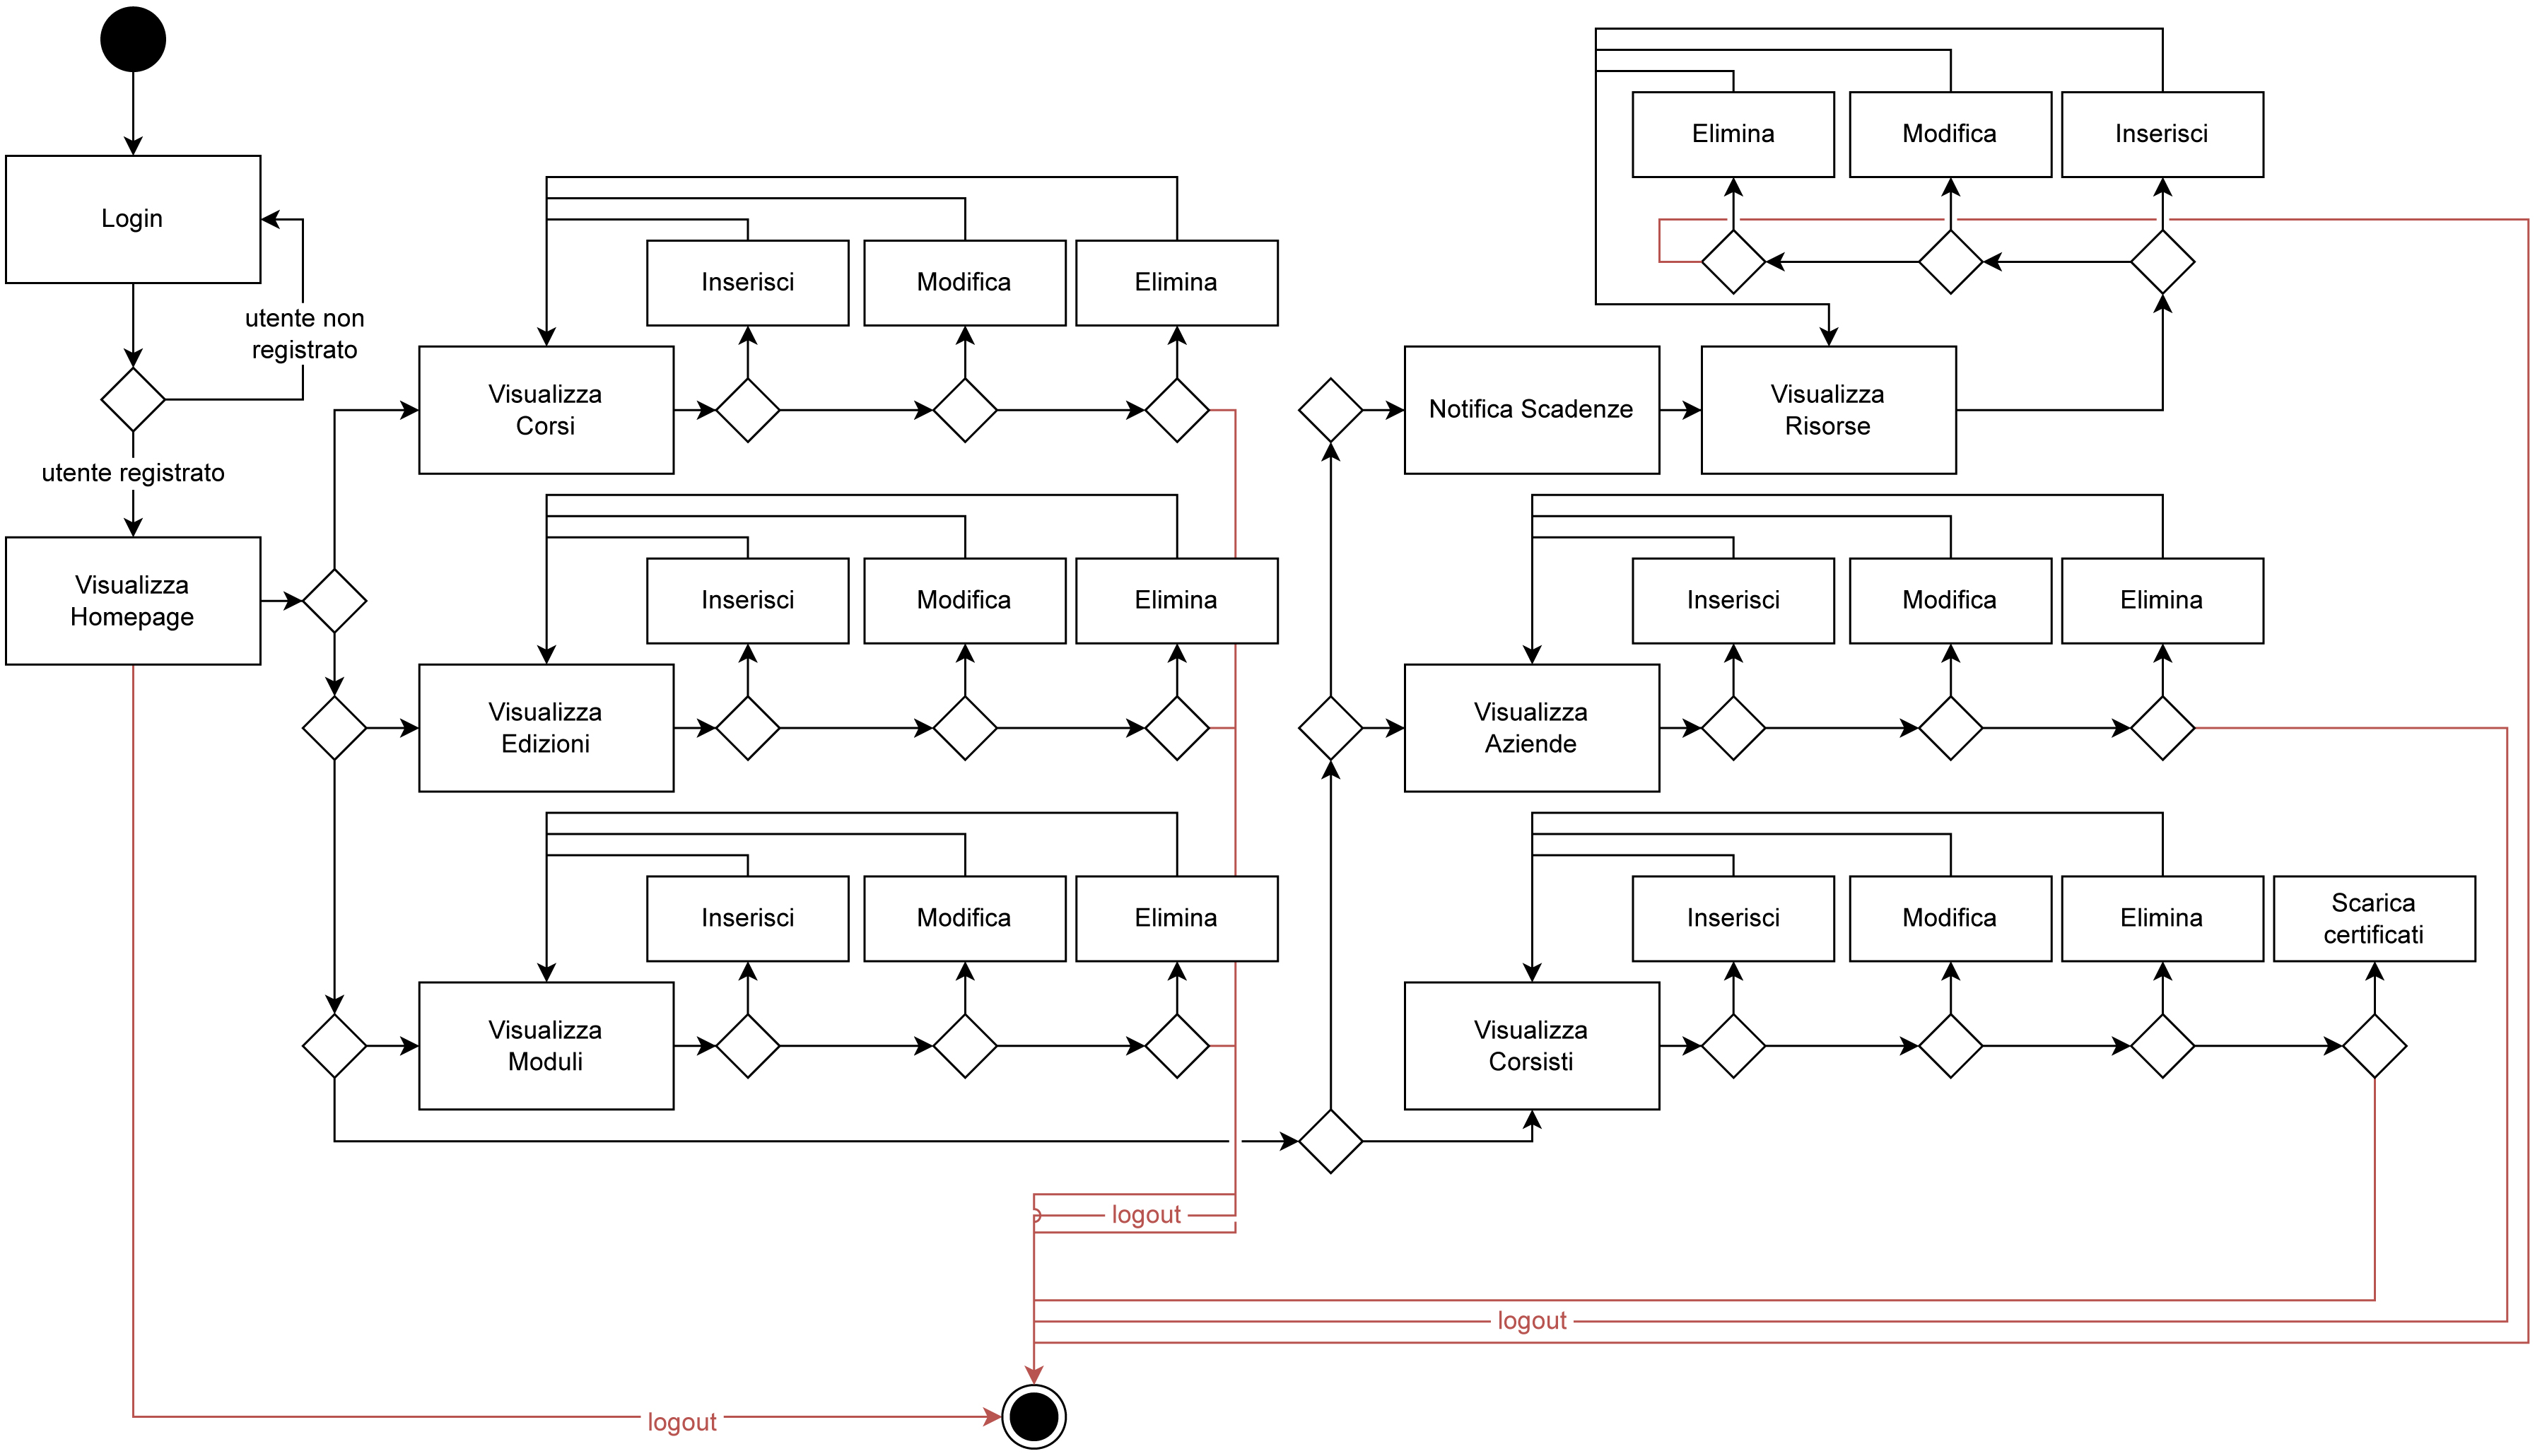
\includegraphics[scale=0.55]{img/Diagramma delle attivita.jpg}
\caption{Diagramma delle attività}
\label{fig:Diagrammadelleattivita}
\end{figure}
\noindent




\section{Analisi del contesto}
\label{sec:contesto}
L'analisi del contesto è quella fase in cui si prendono in considerazione le iterazioni che il software ha con gli altri sistemi in relazione al flusso di informazioni.\\
\newline
Il diagramma in figura \ref{fig:Diagrammadicontesto} rappresenta le interfacce esterne con cui il gestionale comunica. Si individuano due attori (entità che producono o consumano informazioni necessarie per l’elaborazione delle richieste): \textit{Utente Dream} e \textit{Docente Esterno}. Il primo rappresenta l'utente che all'interno dell'azienda utilizza il gestionale mentre il secondo identica un docente che accede alla pagina pubblica per la registrazione a sistema dei suoi dati. Le frecce nel diagramma mostrano i flussi di informazioni.
\subsection{Diagramma di contesto}
\begin{figure}[h]
\centering
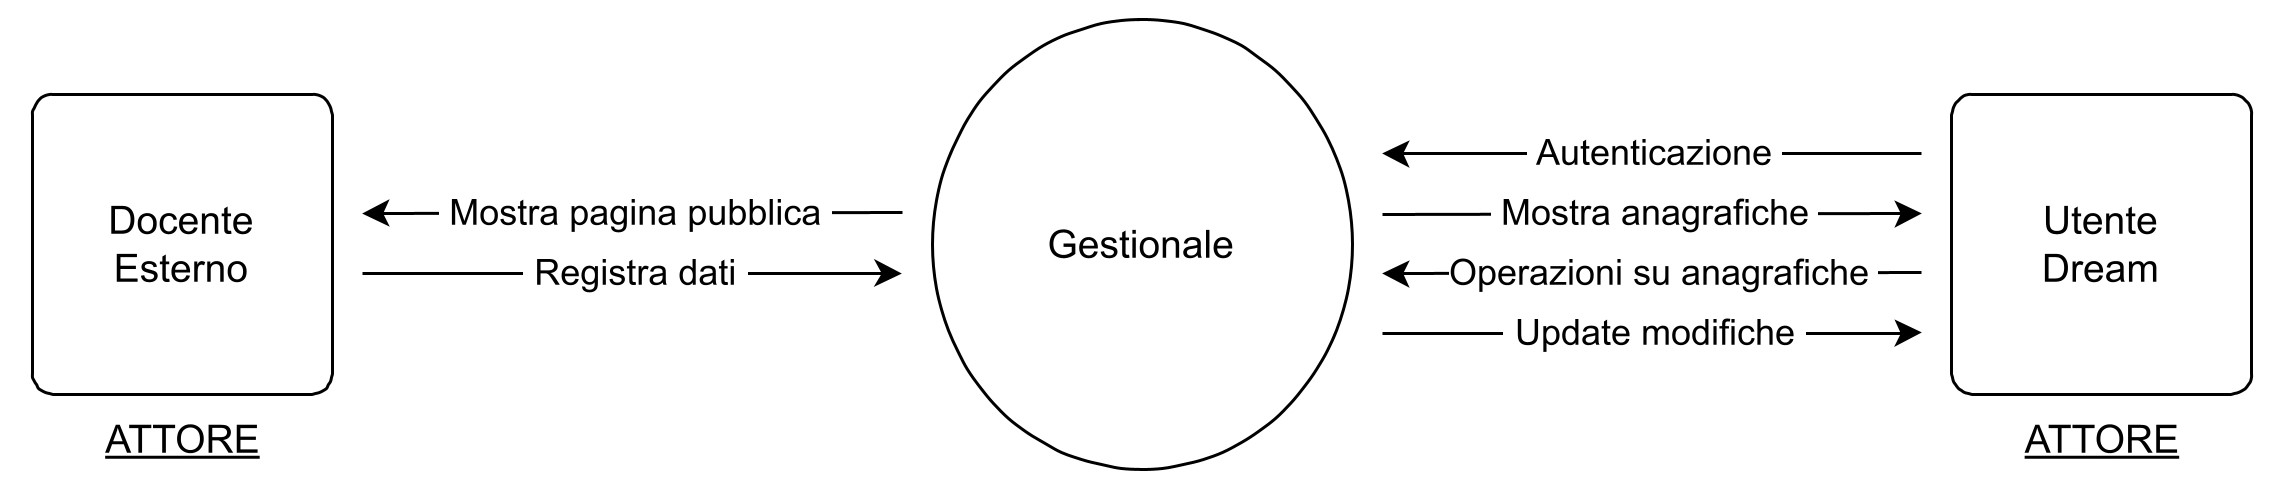
\includegraphics[scale=0.8]{img/Diagramma di Contesto.jpg}
\caption{Diagramma di contesto}
\label{fig:Diagrammadicontesto}
\end{figure}
\noindent


\section{Analisi dei componenti}
\label{sec:componenti}
Questa fase di analisi serve per modellare le connessioni tra i componenti, intesi come singoli moduli del software, in modo da evidenziare le relazioni tra essi e verificare che tutti i compiti che il sistema deve svolgere siano implementati. 
\subsection{Diagramma dei componenti}
In figura \ref{fig:Diagrammadeicomponenti} i rettangoli mappano i componenti mentre le relazioni tra due componenti individuano le interfacce. Le relazioni presentano un semicerchio se l'interfaccia è richiesta da un componente che ne consuma le informazioni; se sono rappresentate con un cerchio allora l'interfaccia in questione è messa a disposizione del componente che ne produce le informazioni.
\begin{figure}[h]
\centering
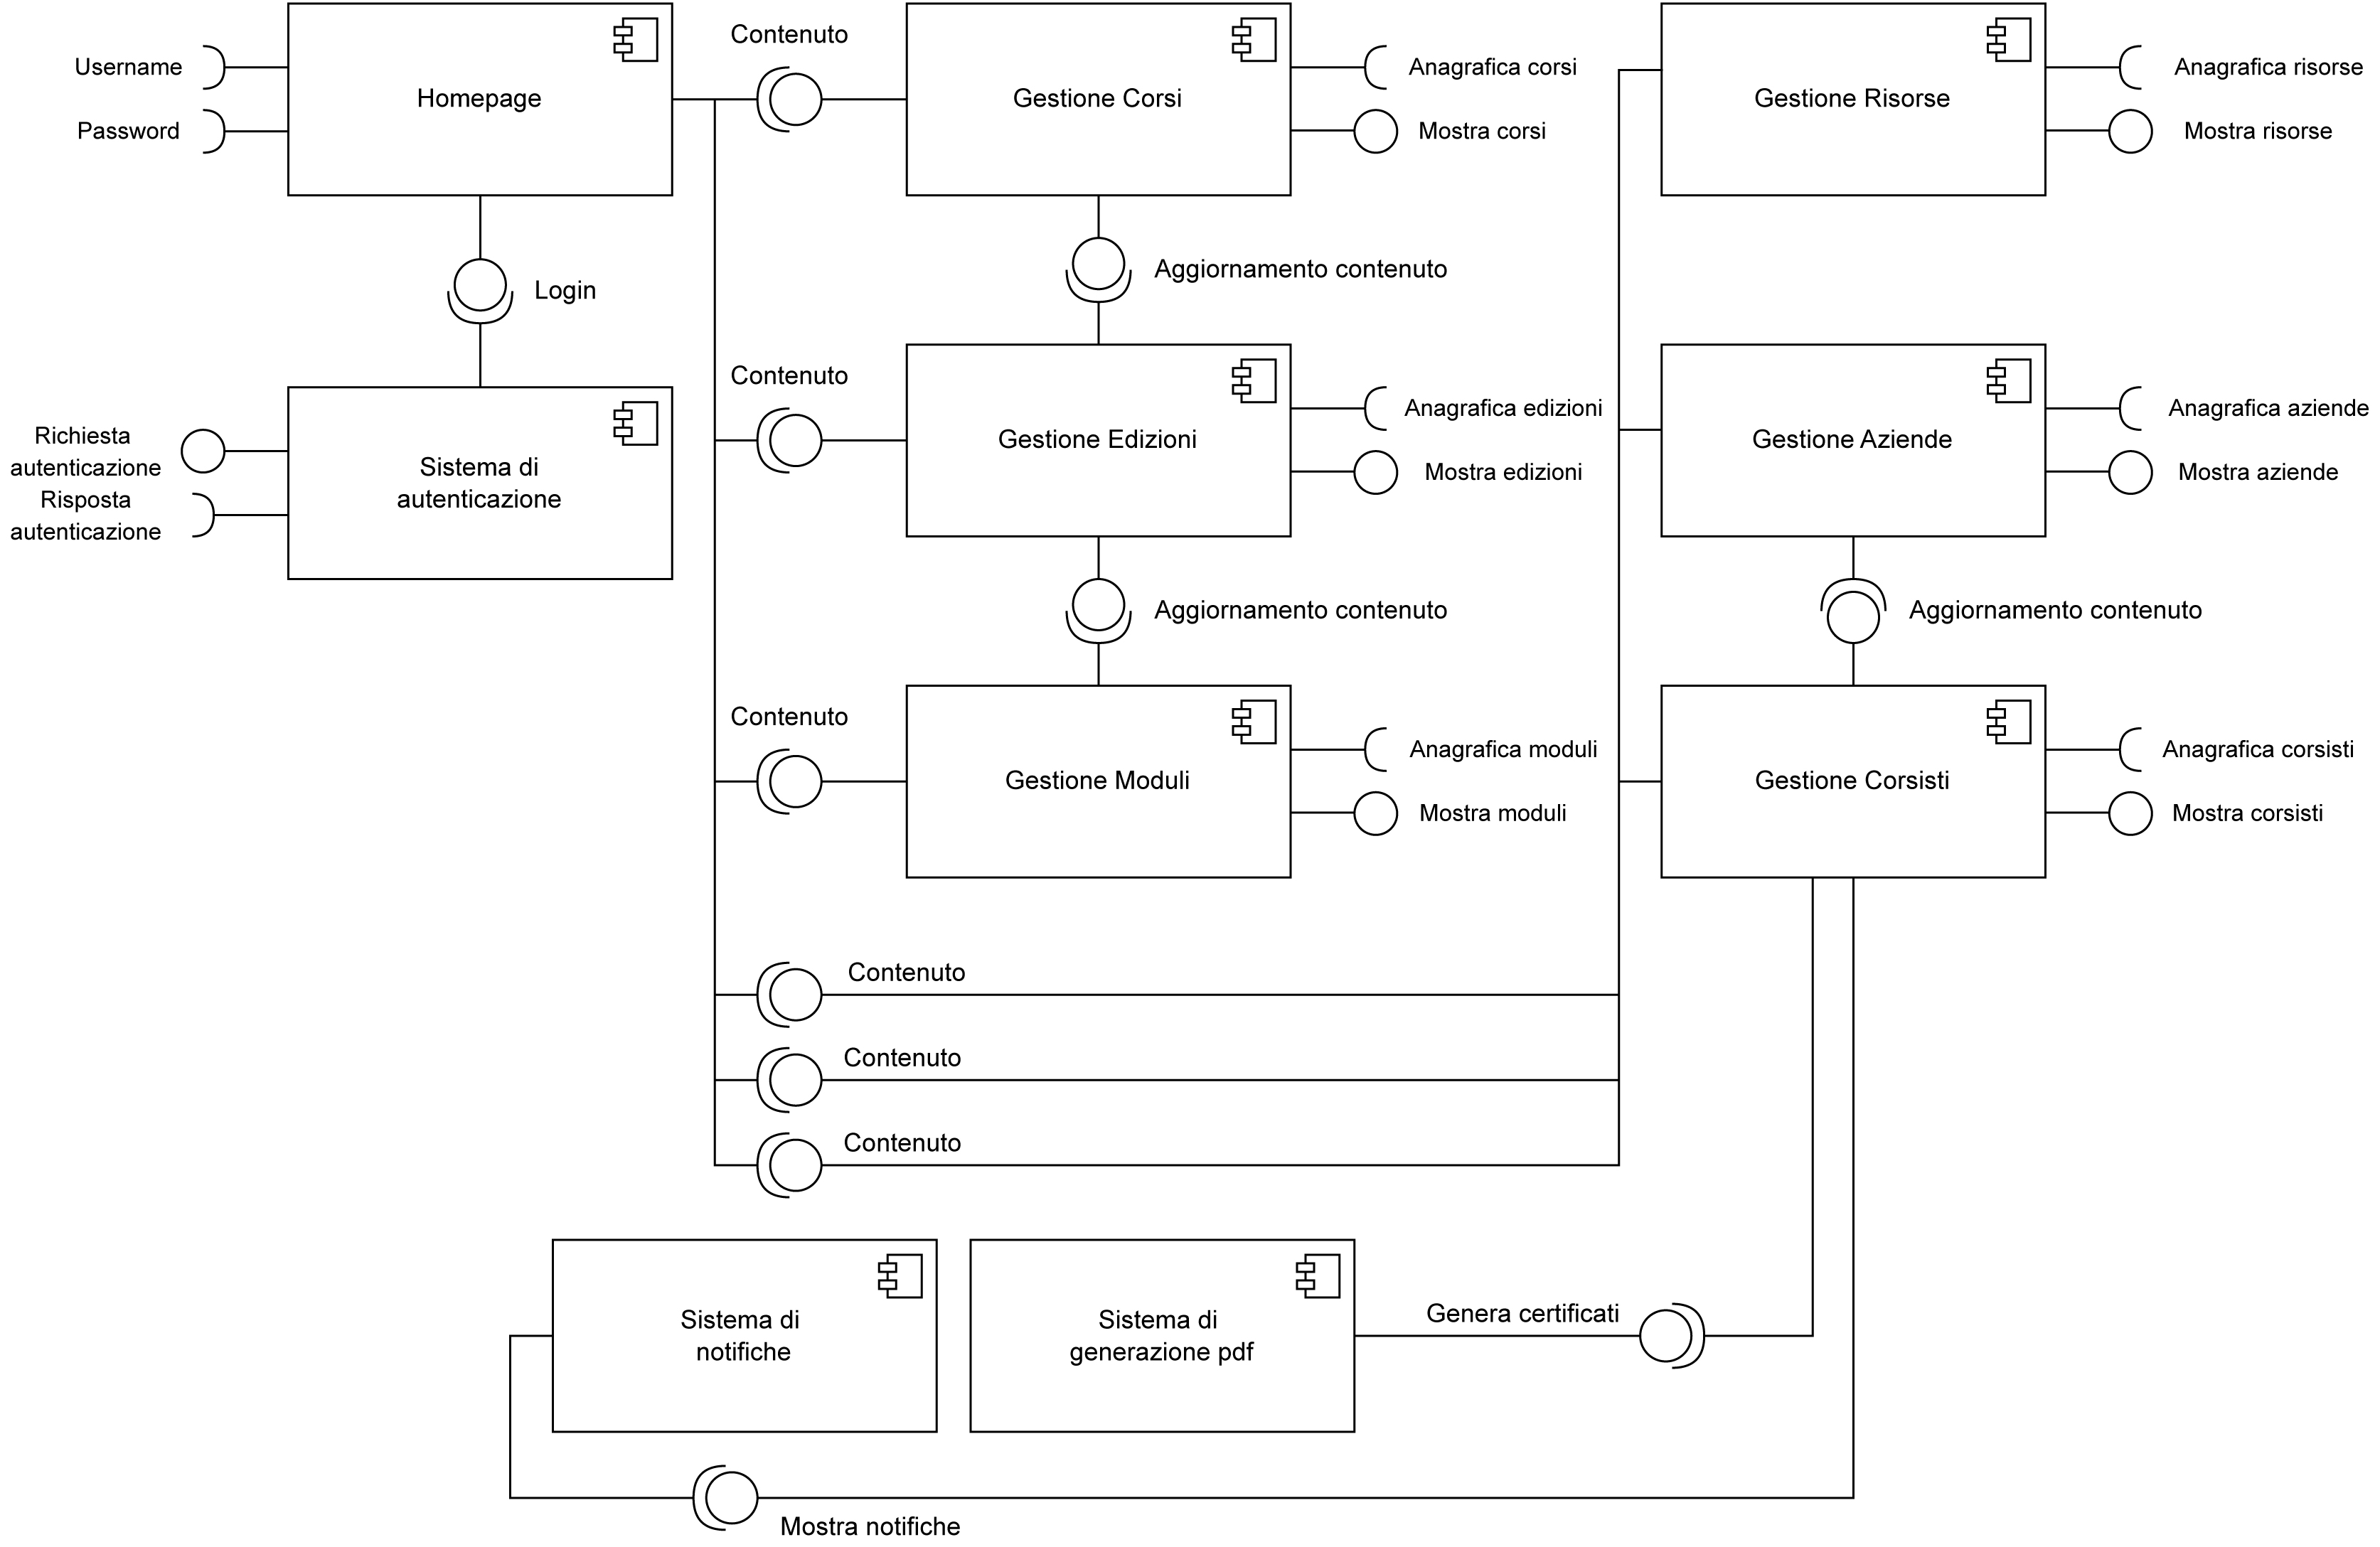
\includegraphics[scale=0.55]{img/Diagramma dei componenti.jpg}
\caption{Diagramma dei componenti}
\label{fig:Diagrammadeicomponenti}
\end{figure}
\clearpage
\newpage
      
      \chapter{Progettazione del database}
\label{cha:database}
I database vengono utilizzati per archiviare e manipolare grandi quantità di informazioni strutturate e non strutturate \cite{database}. L'approccio delle basi di dati racchiude alcune caratteristiche molto importanti, tra cui l'uso di strumenti per auto descrivere i dati collezionati memorizzandone la struttura (meta dati) e fornire la separazione tra programmi e informazioni, ottenendo il vantaggio di poter modificare l'uno o l'altro in maniera indipendente. Una base di dati permette anche di astrarre dai dettagli di memorizzazione dei dati, proponendo diverse rappresentazioni concettuali dei dati e garantisce l'elaborazione delle transizioni multiutente.\\
\newline
Il processo generale di design di un database prevede tre fasi principali:
\begin{enumerate}
    \item Progettazione concettuale
    \item Progettazione logica
    \item Progettazione fisica
\end{enumerate}
\noindent
La prima fase ha come scopo, lavorando sui requisiti raccolti, quello di produrre in output un modello concettuale, ovvero tradurre i problemi e le esigenze emerse in una mappatura semplice da comprendere e comunicare.
Questo tipo di progettazione prevede la definizione di entità (elementi base le cui proprietà sono descritte dagli attributi) e relazioni (che collegano due entità distinte con un particolare significato). L'obiettivo è quindi usare questi schemi (come i diagrammi ER o EER) per semplificare la gestione del database e, al contempo, poter comunicare la struttura generale dei dati richiesta in modo astratto.
La fase successiva serve invece a produrre lo schema logico, partendo da quello appena creato, usando indici e chiavi esterne per definire in modo formale le relazioni tra i dati e ottenere una rappresentazione astratta di una possibile implementazione non vincolata ad alcuna tecnologia specifica. Il modello logico più usato in questo stadio dello sviluppo è quello relazionale. La progettazione fisica, infine, produce lo schema interno della base di dati, in termini di scelta del DBMS (Database Management System) \cite{dbms}, strutture di memorizzazione delle tabelle, organizzazione dei file e dei permessi utente.
\begin{figure}[!hbt]
\centering

\includegraphics[scale=0.50]{img/desing_db.png}
\caption{Processo di progettazione di un database}
\label{fig:design_db}
\end{figure}
\noindent

\section{Tecnologie utilizzate}
\label{sec:dbtech}
Per la corretta gestione e inserimento dei dati, grazie anche all'analisi dei requisiti, è stato progettato il database su cui il sistema appoggia usando come RDBMS (Relational database management system) il servizio MySQL \cite{mysql} in quanto semplice da gestire, gratuito, veloce e, soprattutto, estremamente compatibile con PHP. Per amministrare e configurare il database è stato usato phpMyAdmin \cite{phpmyadmin} mentre per la creazione e modellazione della base di dati si è scelto come strumento MySQL Workbench \cite{mysqlworkbench}.

\section{Diagramma EER}
\label{sec:db}
Un diagramma EER (Extended or Enhanced Entity-Relationship) \cite{eer} è un tipo di schema concettuale che fornisce una rappresentazione visiva della struttura del database sia in fase di creazione, che a processo completo. Oltre agli elementi concettuali di base presenti negli schemi ER tradizionali questo modello aggiunge concetti più sofisticati come sottoclassi e super classi, specializzazioni e generalizzazioni, categorie ed ereditarietà di attributi e relazioni. \\
\newline
In figura \ref{fig:DiagrammaEER} viene mostrato il diagramma EER completo usato per la progettazione del database.
\begin{figure}[!hbt]
\centering
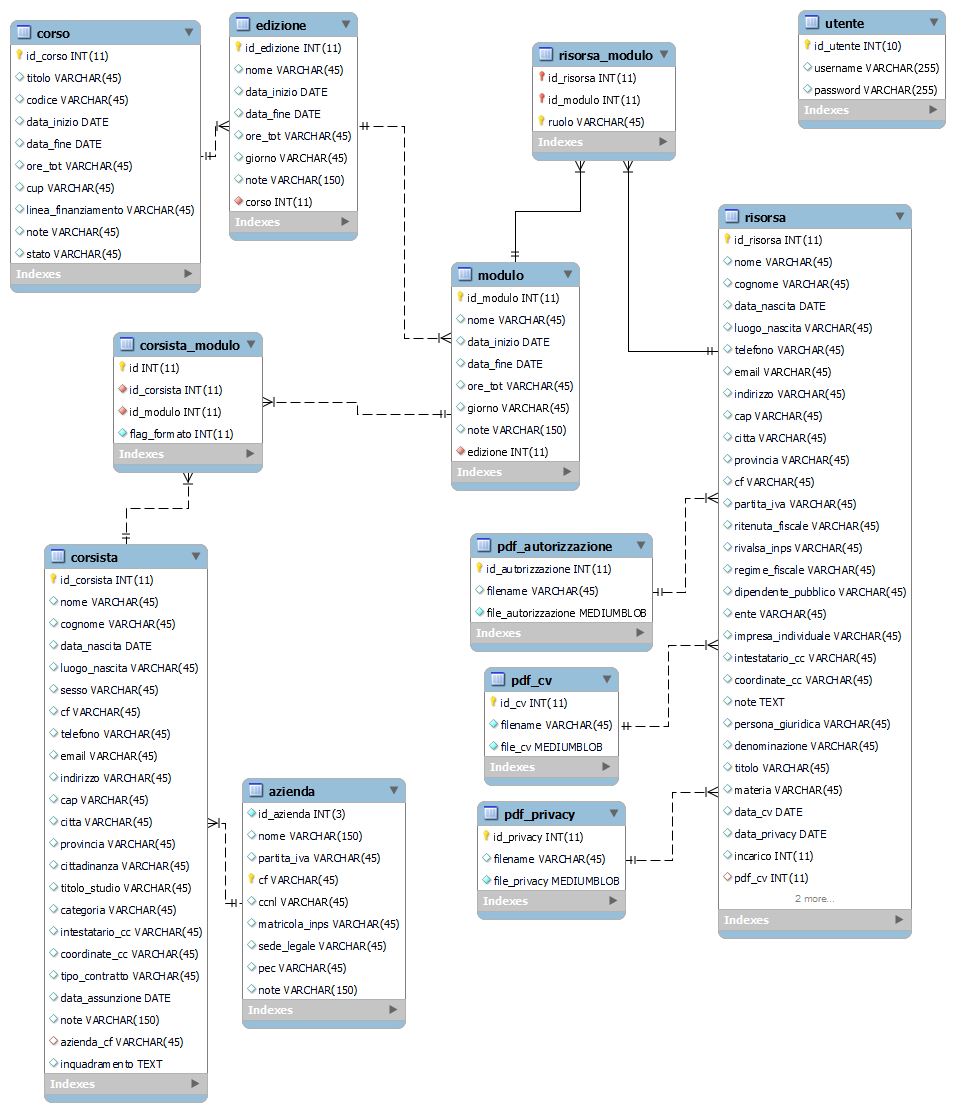
\includegraphics[scale=0.50]{img/EER.png}
\caption{Diagramma EER del database}
\label{fig:DiagrammaEER}
\end{figure}

\section{Normalizzazione e forme normali}
\label{sec:normalizzazione}
Una tecnica usata per la verifica dei risultati della progettazione di una base di dati è la normalizzazione, che consiste nel trasformare schemi non normalizzati in schemi che soddisfano una forma normale. Lo scopo è quindi passare per ogni relazione, da una con ridondanze a una assente di difetti, il che è sinonimo di qualità. Le anomalie delle relazioni possono essere risolte seguendo le forme normali, in particolare la Prima Forma Normale (1NF) richiede che tutti gli attributi dello schema non siano composti o multi valore; vale invece la Seconda Forma Normale (2NF) se, oltre a essere in 1NF, ogni attributo non appartenente a nessuna chiave dipende completamente da ogni chiave (quindi non dipende da una parte di chiave). I requisiti della Terza forma normale (3NF) sono che, oltre a valere la 2NF, tutti gli attributi non chiave devono dipendere direttamente dalla chiave, quindi non possono esserci attributi dipendenti da altri attributi che non sono presenti in chiave. La Forma Normale di Boyce-Codd (BCNF) prevede, di fatto, che ogni attributo dal quale ne dipendono altri possa svolgere la funzione di chiave, oltre a essere in 1NF.\\
\newline
Per quanto riguarda il modello elaborato per il progetto, la Prima Forma Normale è già parte integrante della definizione formale di relazione nel modello relazionale. Non essendoci dipendenze parziali tra attributi dalle varie chiavi, anche la Seconda Forma Normale è rispettata. Non vale invece la 3 NF in quanto esistono dipendenze tra le colonne di una tabella basate su attributi che non sono chiave primaria; ad esempio nella tabella \verb|corsista| è presente il campo \verb|data_assunzione| che non è subordinato alla chiave primaria della tabella. Sono perciò presenti attributi non chiave che dipendono transitivamente dalla chiave. Il livello di normalizzazione usato è quindi quello di 2NF. Uno dei presupposti per un futuro rilascio del sistema potrebbe essere quello di arrivare a rispettare la Terza forma normale adattando di conseguenza le relazioni della base di dati.



\section{Traduzione in SQL}
Durante la fase di progettazione logica, SQL (Structured Query Language) è il linguaggio usato dai modelli relazionali per permettere le operazioni di creazione o modifica dello schema (DDL: Data Definition Language) e di interrogazione, inserimento, modifica o eliminazione dei dati (DML: Data Manipulation Language). A titolo di esempio si riporta il codice in SQL per la creazione della tabella \verb|modulo| della base di dati (listing \ref{code:sql}).

\begin{listing}[h]
\begin{minted}{SQL}
CREATE TABLE `modulo` (
  `id_modulo` int(11) NOT NULL,
  `nome` varchar(45) DEFAULT NULL,
  `data_inizio` date DEFAULT NULL,
  `data_fine` date DEFAULT NULL,
  `ore_tot` varchar(45) DEFAULT NULL,
  `giorno` varchar(45) DEFAULT NULL,
  `note` varchar(150) DEFAULT NULL,
  `edizione` int(11) NOT NULL
) ENGINE=InnoDB DEFAULT CHARSET=utf8mb4;
-- Indici per le tabelle `modulo`
ALTER TABLE `modulo`
  ADD PRIMARY KEY (`id_modulo`),
  ADD KEY `fk_modulo_edizione1` (`edizione`);
-- Limiti per la tabella `modulo`
ALTER TABLE `modulo`
  ADD CONSTRAINT `fk_modulo_edizione1` FOREIGN KEY
  (`edizione`) REFERENCES `edizione` (`id_edizione`)
  ON DELETE NO ACTION ON UPDATE NO ACTION;
\end{minted}
\caption{codice SQL per la creazione della tabella \textit{Modulo}}
\label{code:sql}
\end{listing}


\clearpage
\newpage

   %\newpage
   
    \clearpage
\newpage
\chapter{Sviluppo e output}
\label{cha:789}
Questo capitolo analizza il progetto dal punto di vista dell'implementazione del gestionale.\\
Verranno introdotte le tecnologie utilizzare e la strutturazione dei moduli sviluppati, per poi allegare alla descrizione del funzionamento alcuni screenshots delle pagine principali e alcuni script di codice PHP relativi a funzionalità di rilievo.



\section{Tecnologie utilizzate}
\label{sec:tecnologie}
L'intero progetto segue le basi dello stack LAMP \cite{lamp} (Linux, Apache, MySQL, e PHP). Come piattaforma per l'implementazione in locale è stato scelto XAMPP \cite{xampp} che fornisce un web server Apache, database MySQL e l'interprete PHP e permette, inoltre, la gestione completa dei database. Il progetto è stato poi trasferito su Aruba \cite{aruba}, società italiana che offre servizi di data center, web hosting, email e registrazione di nomi di dominio.
Per lo sviluppo lato server PHP8.0 \cite{php} è quindi il linguaggio di scripting di riferimento, HTML \cite{html}\cite{html2} è invece usato per la visualizzazione delle pagine lato client.
Per la parte di programmazione asincrona \cite{asincrona} la maggior parte delle funzioni poggia sulla libreria jQuery \cite{jquery} per semplificare il lavoro con AJAX \cite{ajax}. Data l'importanza della presentazione e gestione dei dati legati alle varie anagrafiche è stato usato il plug-in DataTables \cite{datatables}.
Per la formattazione oltre a CSS \cite{css} si è scelto il framework Bootstrap \cite{bootstrap} nella versione 5.0. 

\section{Struttura del progetto}
\label{sec:struttura}
Per lo sviluppo del gestionale si è proseguito individuando i singoli moduli principali e implementando per ognuno le funzioni richieste. Di seguito si riporta quindi la struttura del progetto, in termini di componenti.
\begin{lstlisting}[language=c]
- config
- modules
	- attestati
	- aziende
	- corsi
	- corsisti
	- edizioni
	- homepage
	- login
	- moduli
	- public
	- risorse
		- scadenze
	- ruoli
- lib
\end{lstlisting}

\section{Login e Homepage}
Per prima cosa il gestionale mostra all'utente la pagina di login (figura \ref{fig:login}) per l'accesso con username e password. Il sistema interroga il database e in caso di successo reindirizza l'utente alla \textit{Homepage} (figura \ref{fig:homepage}) impostando la sessione come attiva. In questo modo ogni pagina sarà accessibile a meno di logout; alla scadenza della sessione l'utente dovrà effettuare nuovamente l'accesso. Dalla homepage è quindi possibile accedere a ogni sezione del sistema.
\begin{figure}[!hbt]
\centering
\begin{minipage}[b]{0.3\textwidth}
    \fcolorbox{gray}{white}{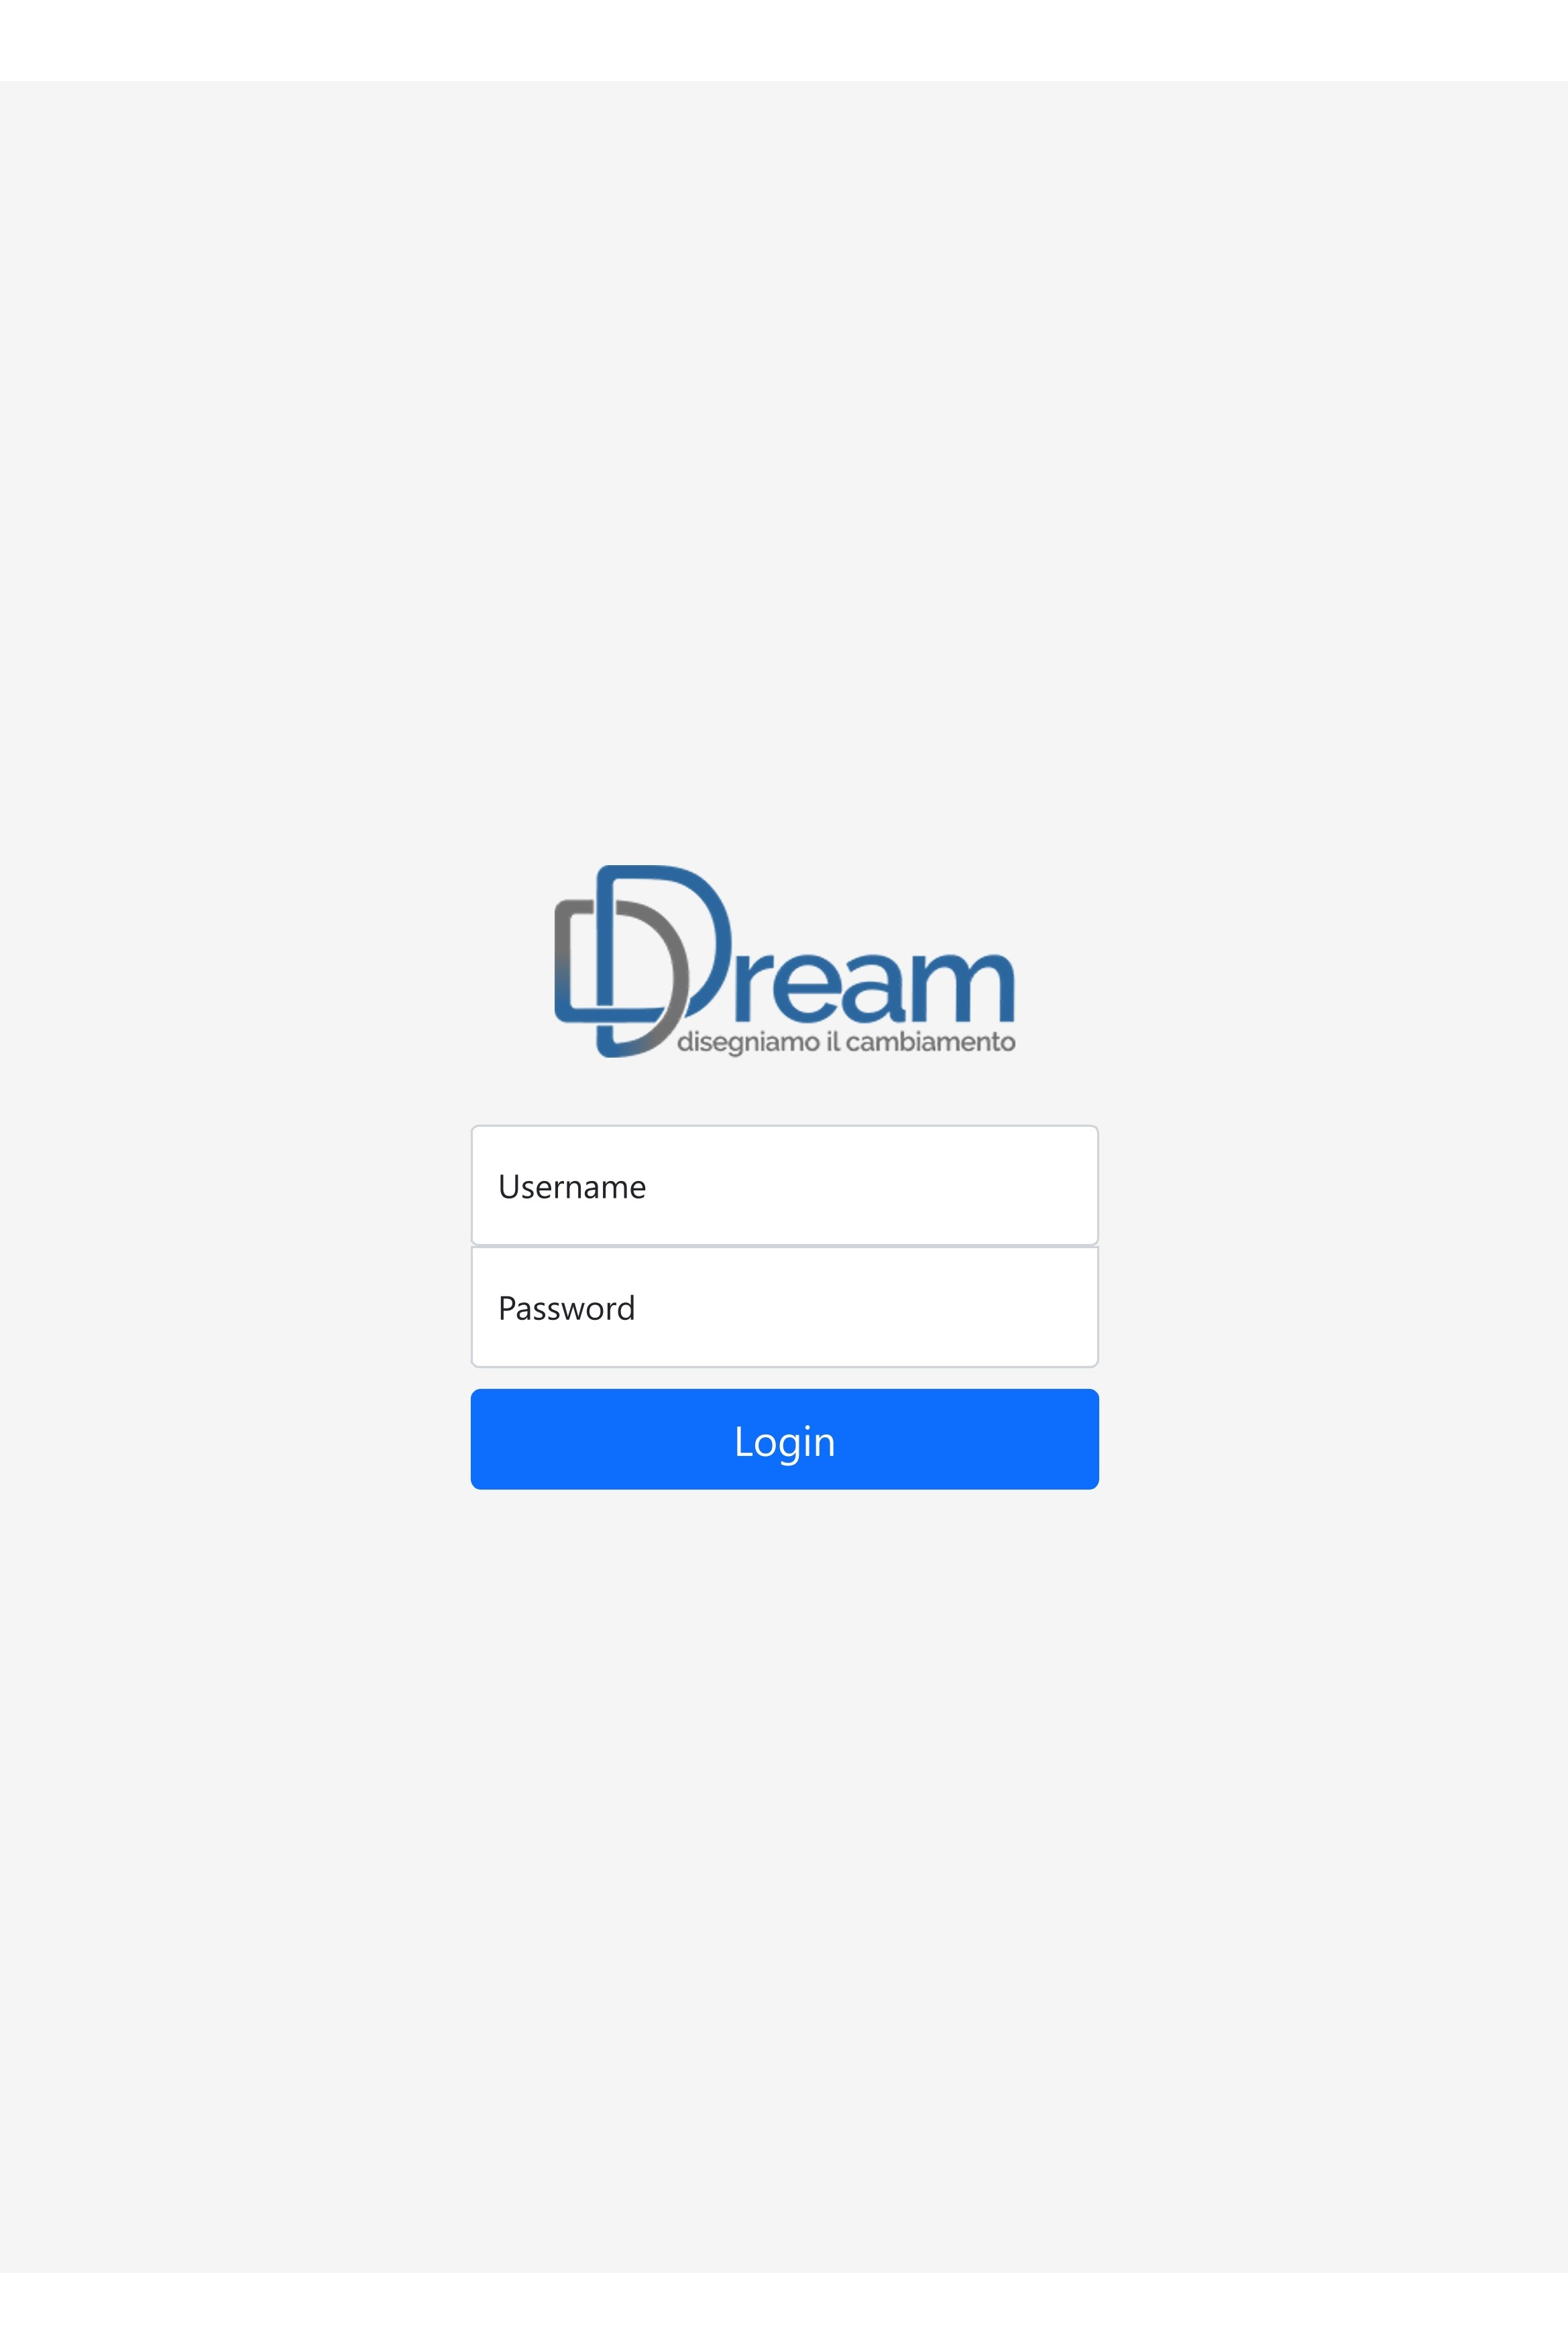
\includegraphics[width=\textwidth]{img/screen/Login-1.jpg}}
    \caption{Login (screenshot)}
    \label{fig:login}
  \end{minipage}
  \hfill
  \begin{minipage}[b]{0.65\textwidth}
    \fcolorbox{gray}{white}{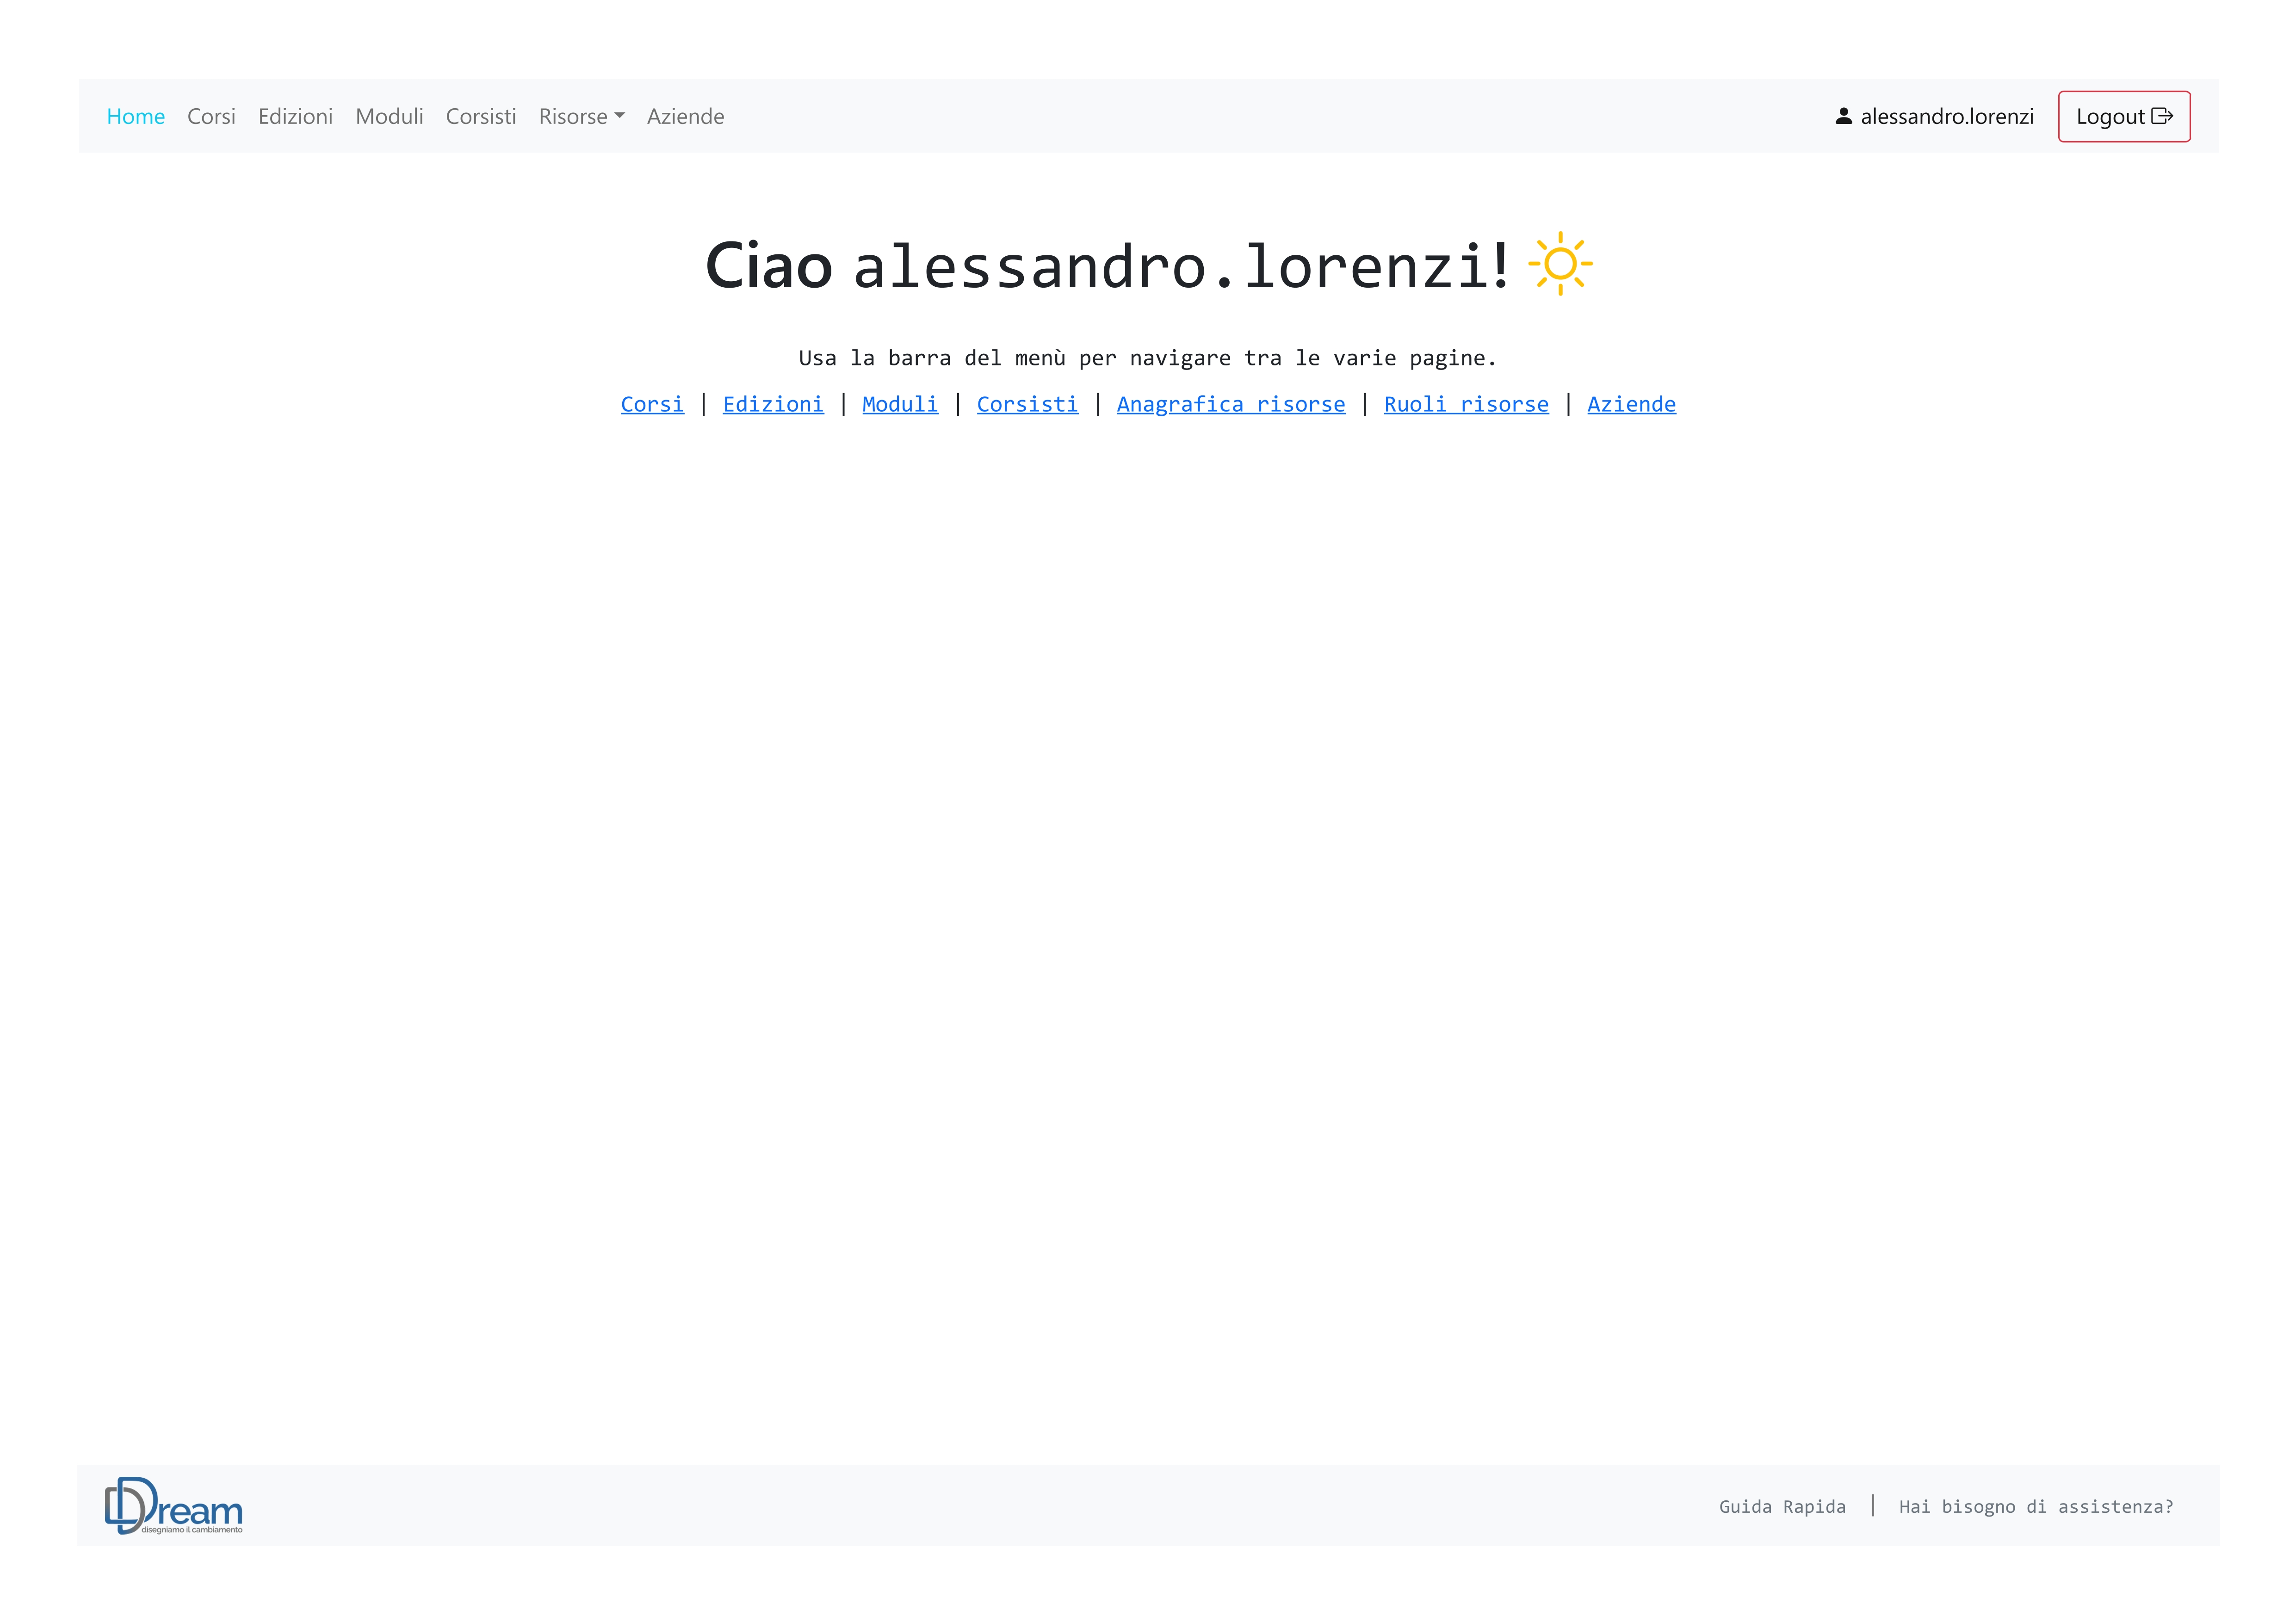
\includegraphics[width=\textwidth]{img/screen/Home-1.jpg}}
    \caption{Homepage (screenshot)}
    \label{fig:homepage}
  \end{minipage}
\end{figure}
\noindent
Le pagine \textit{Corsi}, \textit{Edizioni} e \textit{Moduli} permettono la gestione delle rispettive anagrafiche. L'utente può visualizzare in modo strutturato e navigabile le varie informazioni, aggiungere nuovi dati o eliminare i componenti presenti.

\section{Pagina Moduli}
La pagina \textit{Moduli} (figura \ref{fig:moduli}), un esempio tra le varie pagine di anagrafiche, fornisce una tabella che può essere filtrata per corso ed edizione. Ogni modulo può essere modificato e, se possibile, eliminato; l'utente può anche creare un nuovo modulo. 
\begin{figure}[!hbt]
\centering
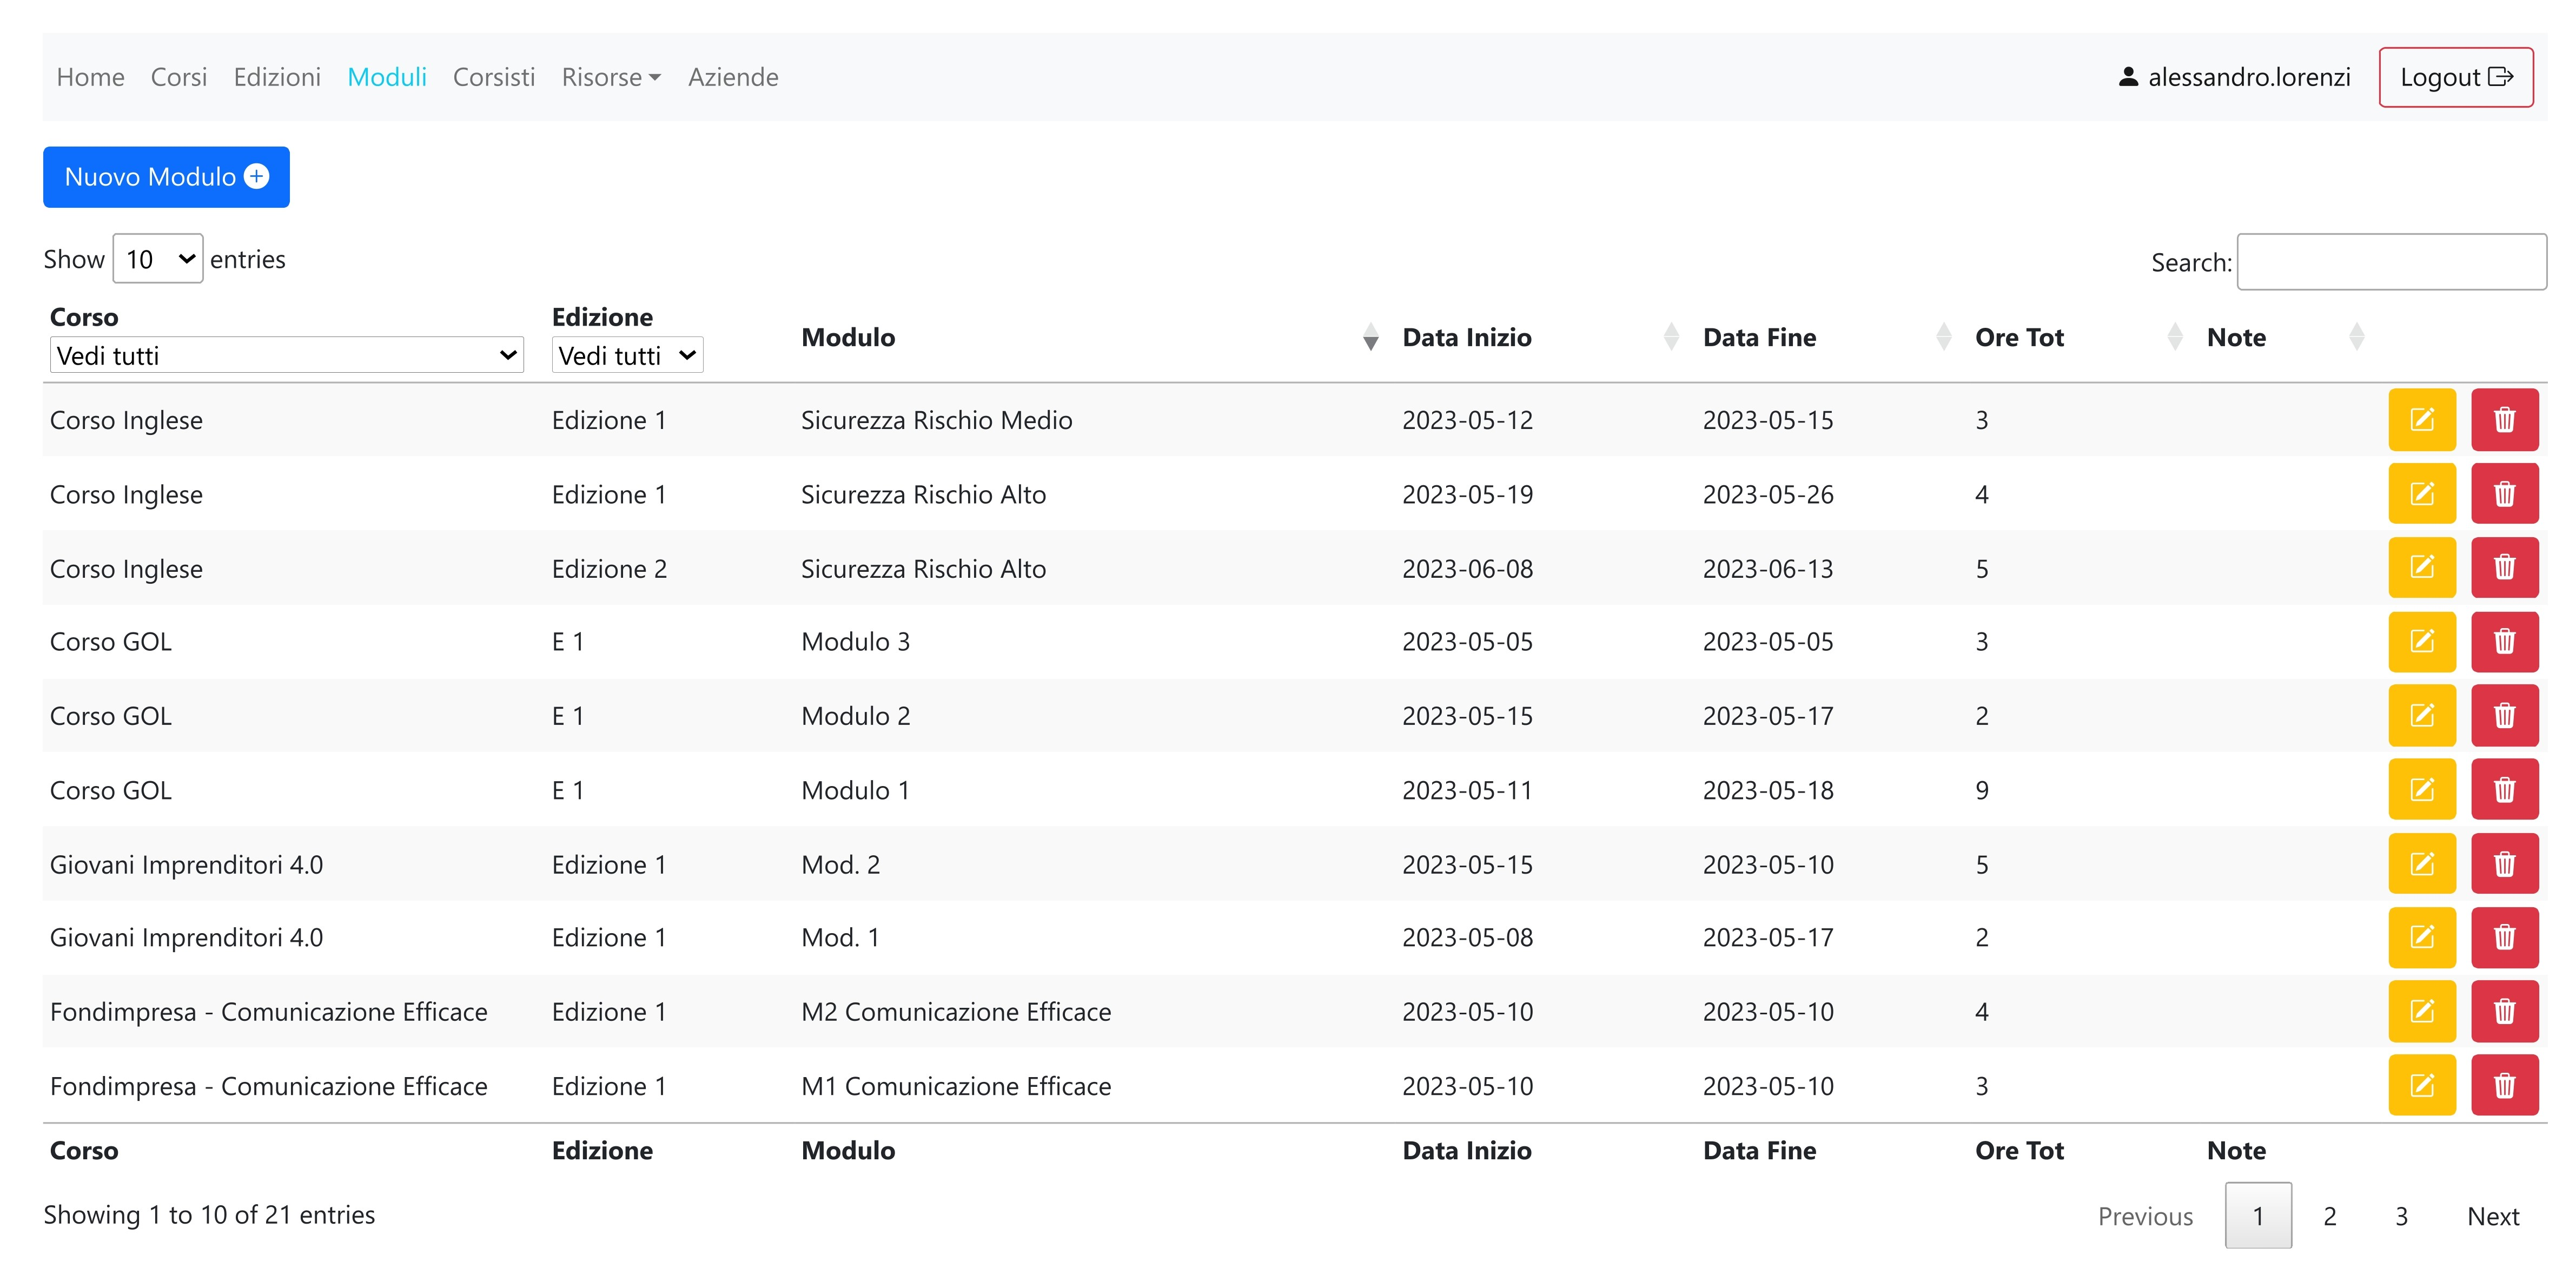
\includegraphics[scale=0.35]{img/screen/Moduli_tabella-1.jpg}
\caption{Pagina Moduli (screenshot)}
\label{fig:moduli}
\end{figure}
\newline
In figura \ref{fig:operazioni_moduli} si mostrano le operazioni di creazione e modifica di un modulo. In caso di creazione di un nuovo modulo il sistema popola due menù a discesa selezionabili che si aggiornano in base alle scelte fatte. Una volta compilati i campi obbligatori la nuova entità viene caricata nel database e la pagina di visualizzazione si aggiorna. In caso di modifica invece uno script in JavaScript precompila i campi del modulo selezionato e, una volta confermata la variazione, il sistema esegue l'aggiornamento delle informazioni aggiornando la tabella. Se l'utente dovesse scegliere di eliminare un elemento il gestionale controlla prima che non ci siano vincoli di integrità violati (ad esempio nel caso di moduli l'eliminazione è possibile solo se non ci sono corsisti e/o risorse associate a esso) e successivamente esegue la cancellazione o restituisce un messaggio di errore senza procedere.
\begin{figure}[!hbt]
\centering
% \begin{subfigure}{0.8\textwidth}
%      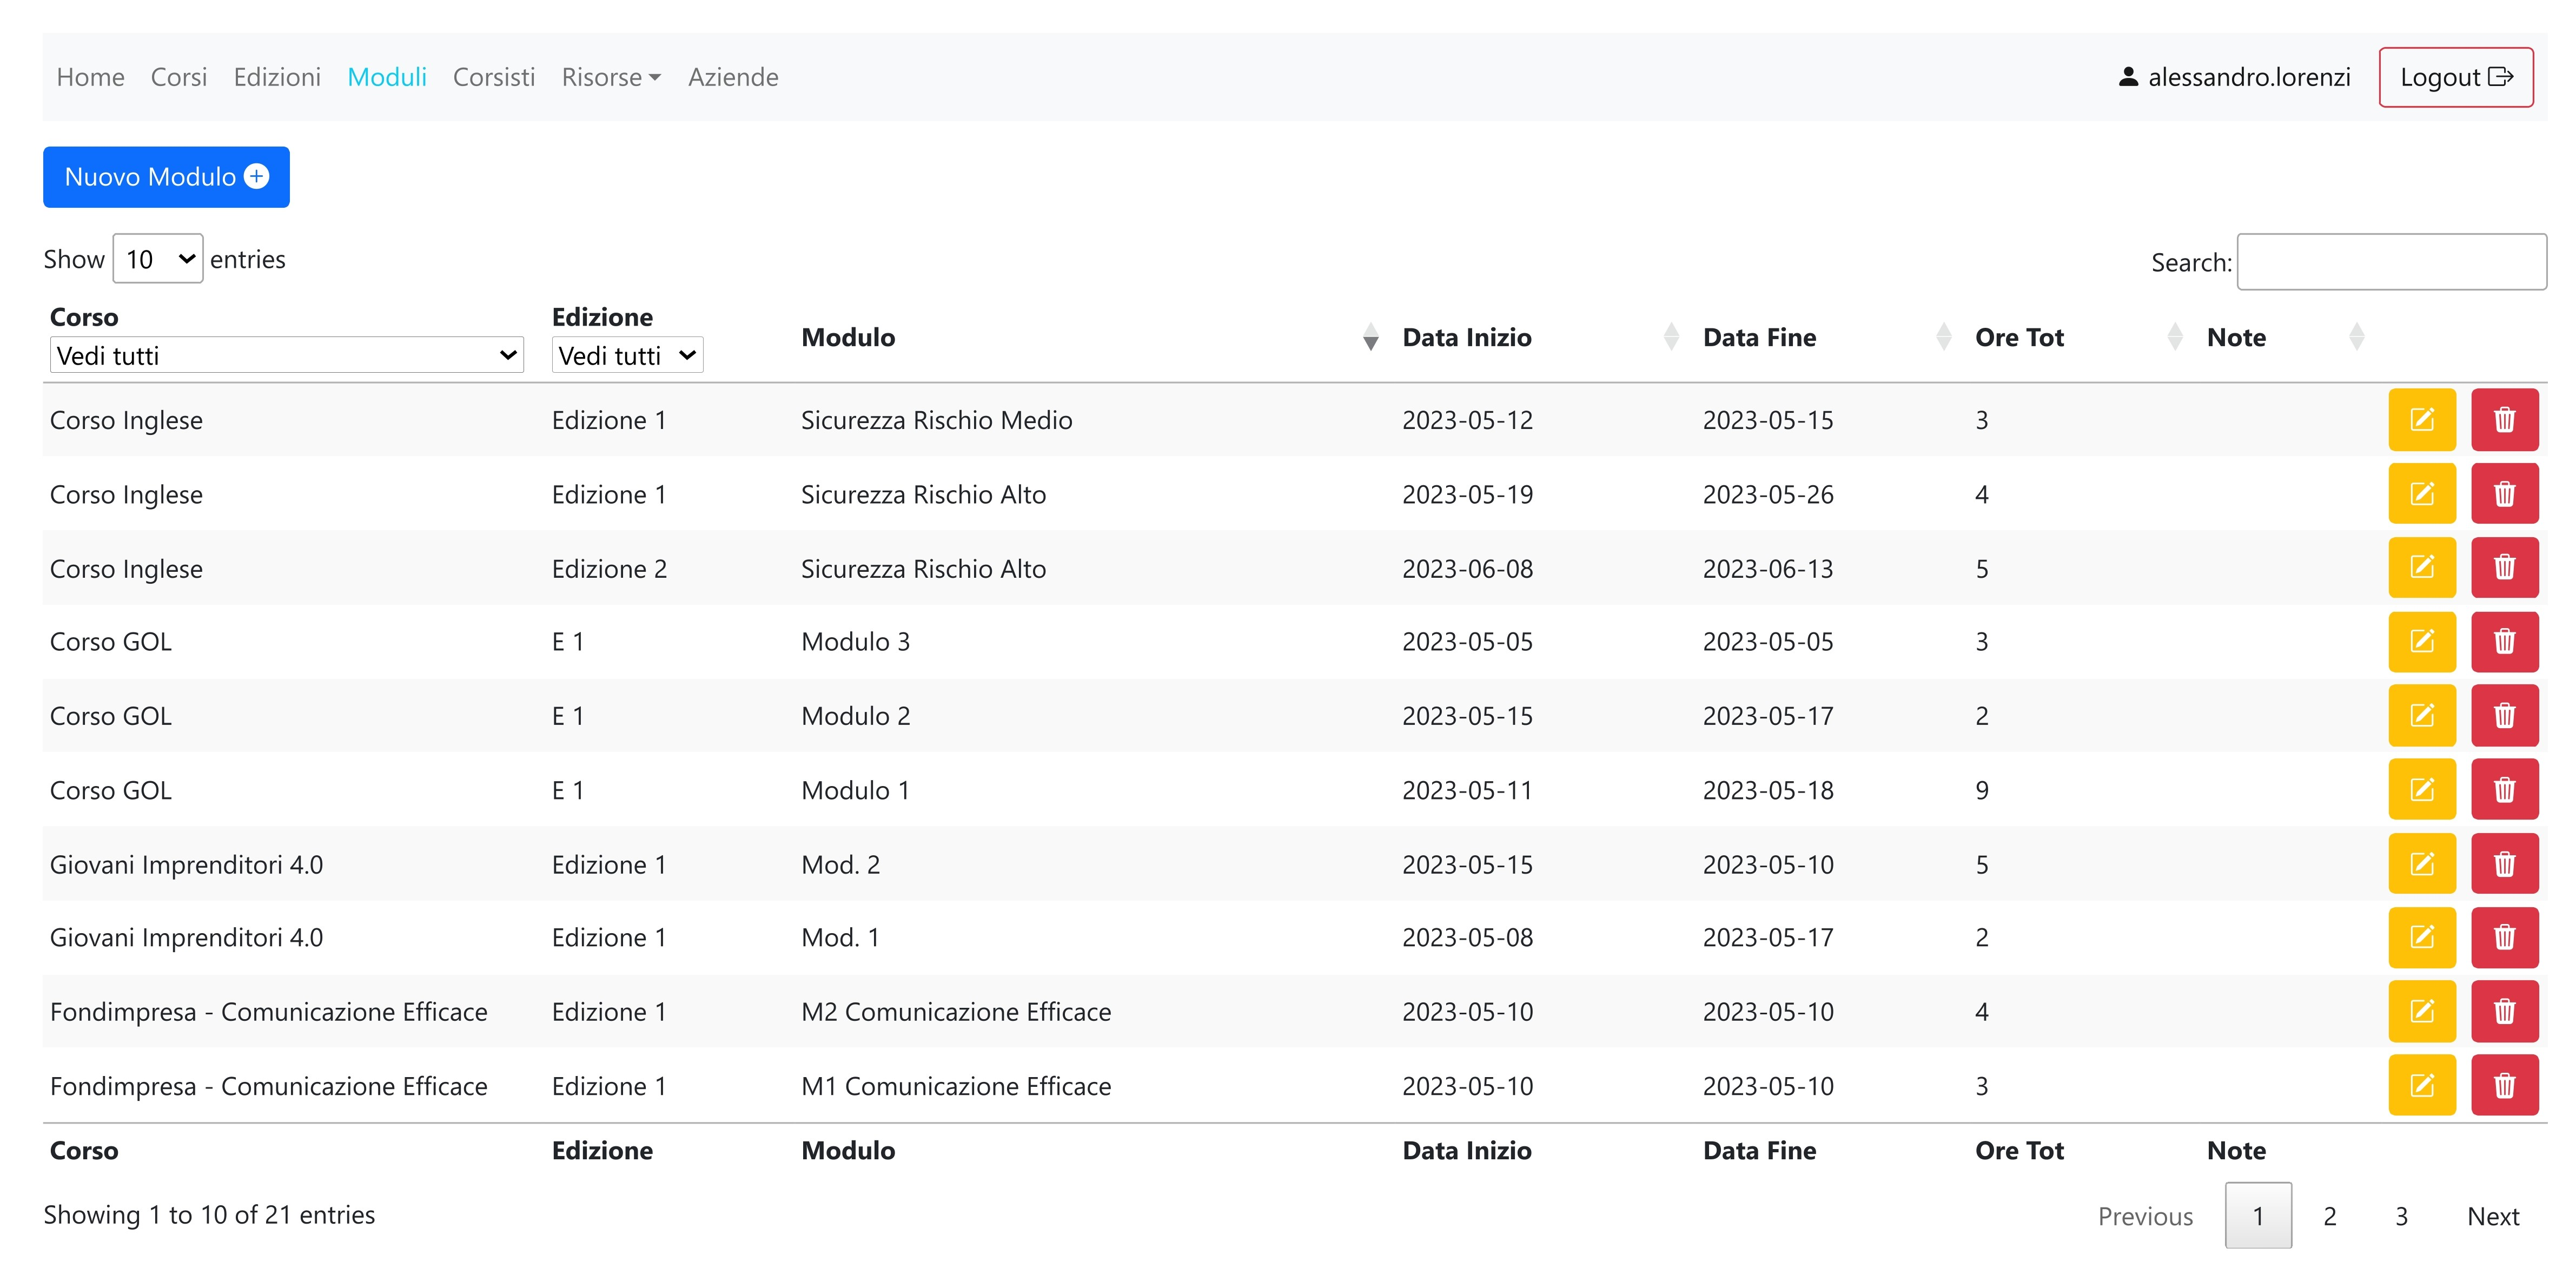
\includegraphics[width=\textwidth]{img/screen/Moduli_tabella-1.jpg}
%      \caption{Pagina Moduli}
%      \label{fig:nuovo_modulo}
%  \end{subfigure}
%  \hfill
 \begin{subfigure}{0.49\textwidth}
     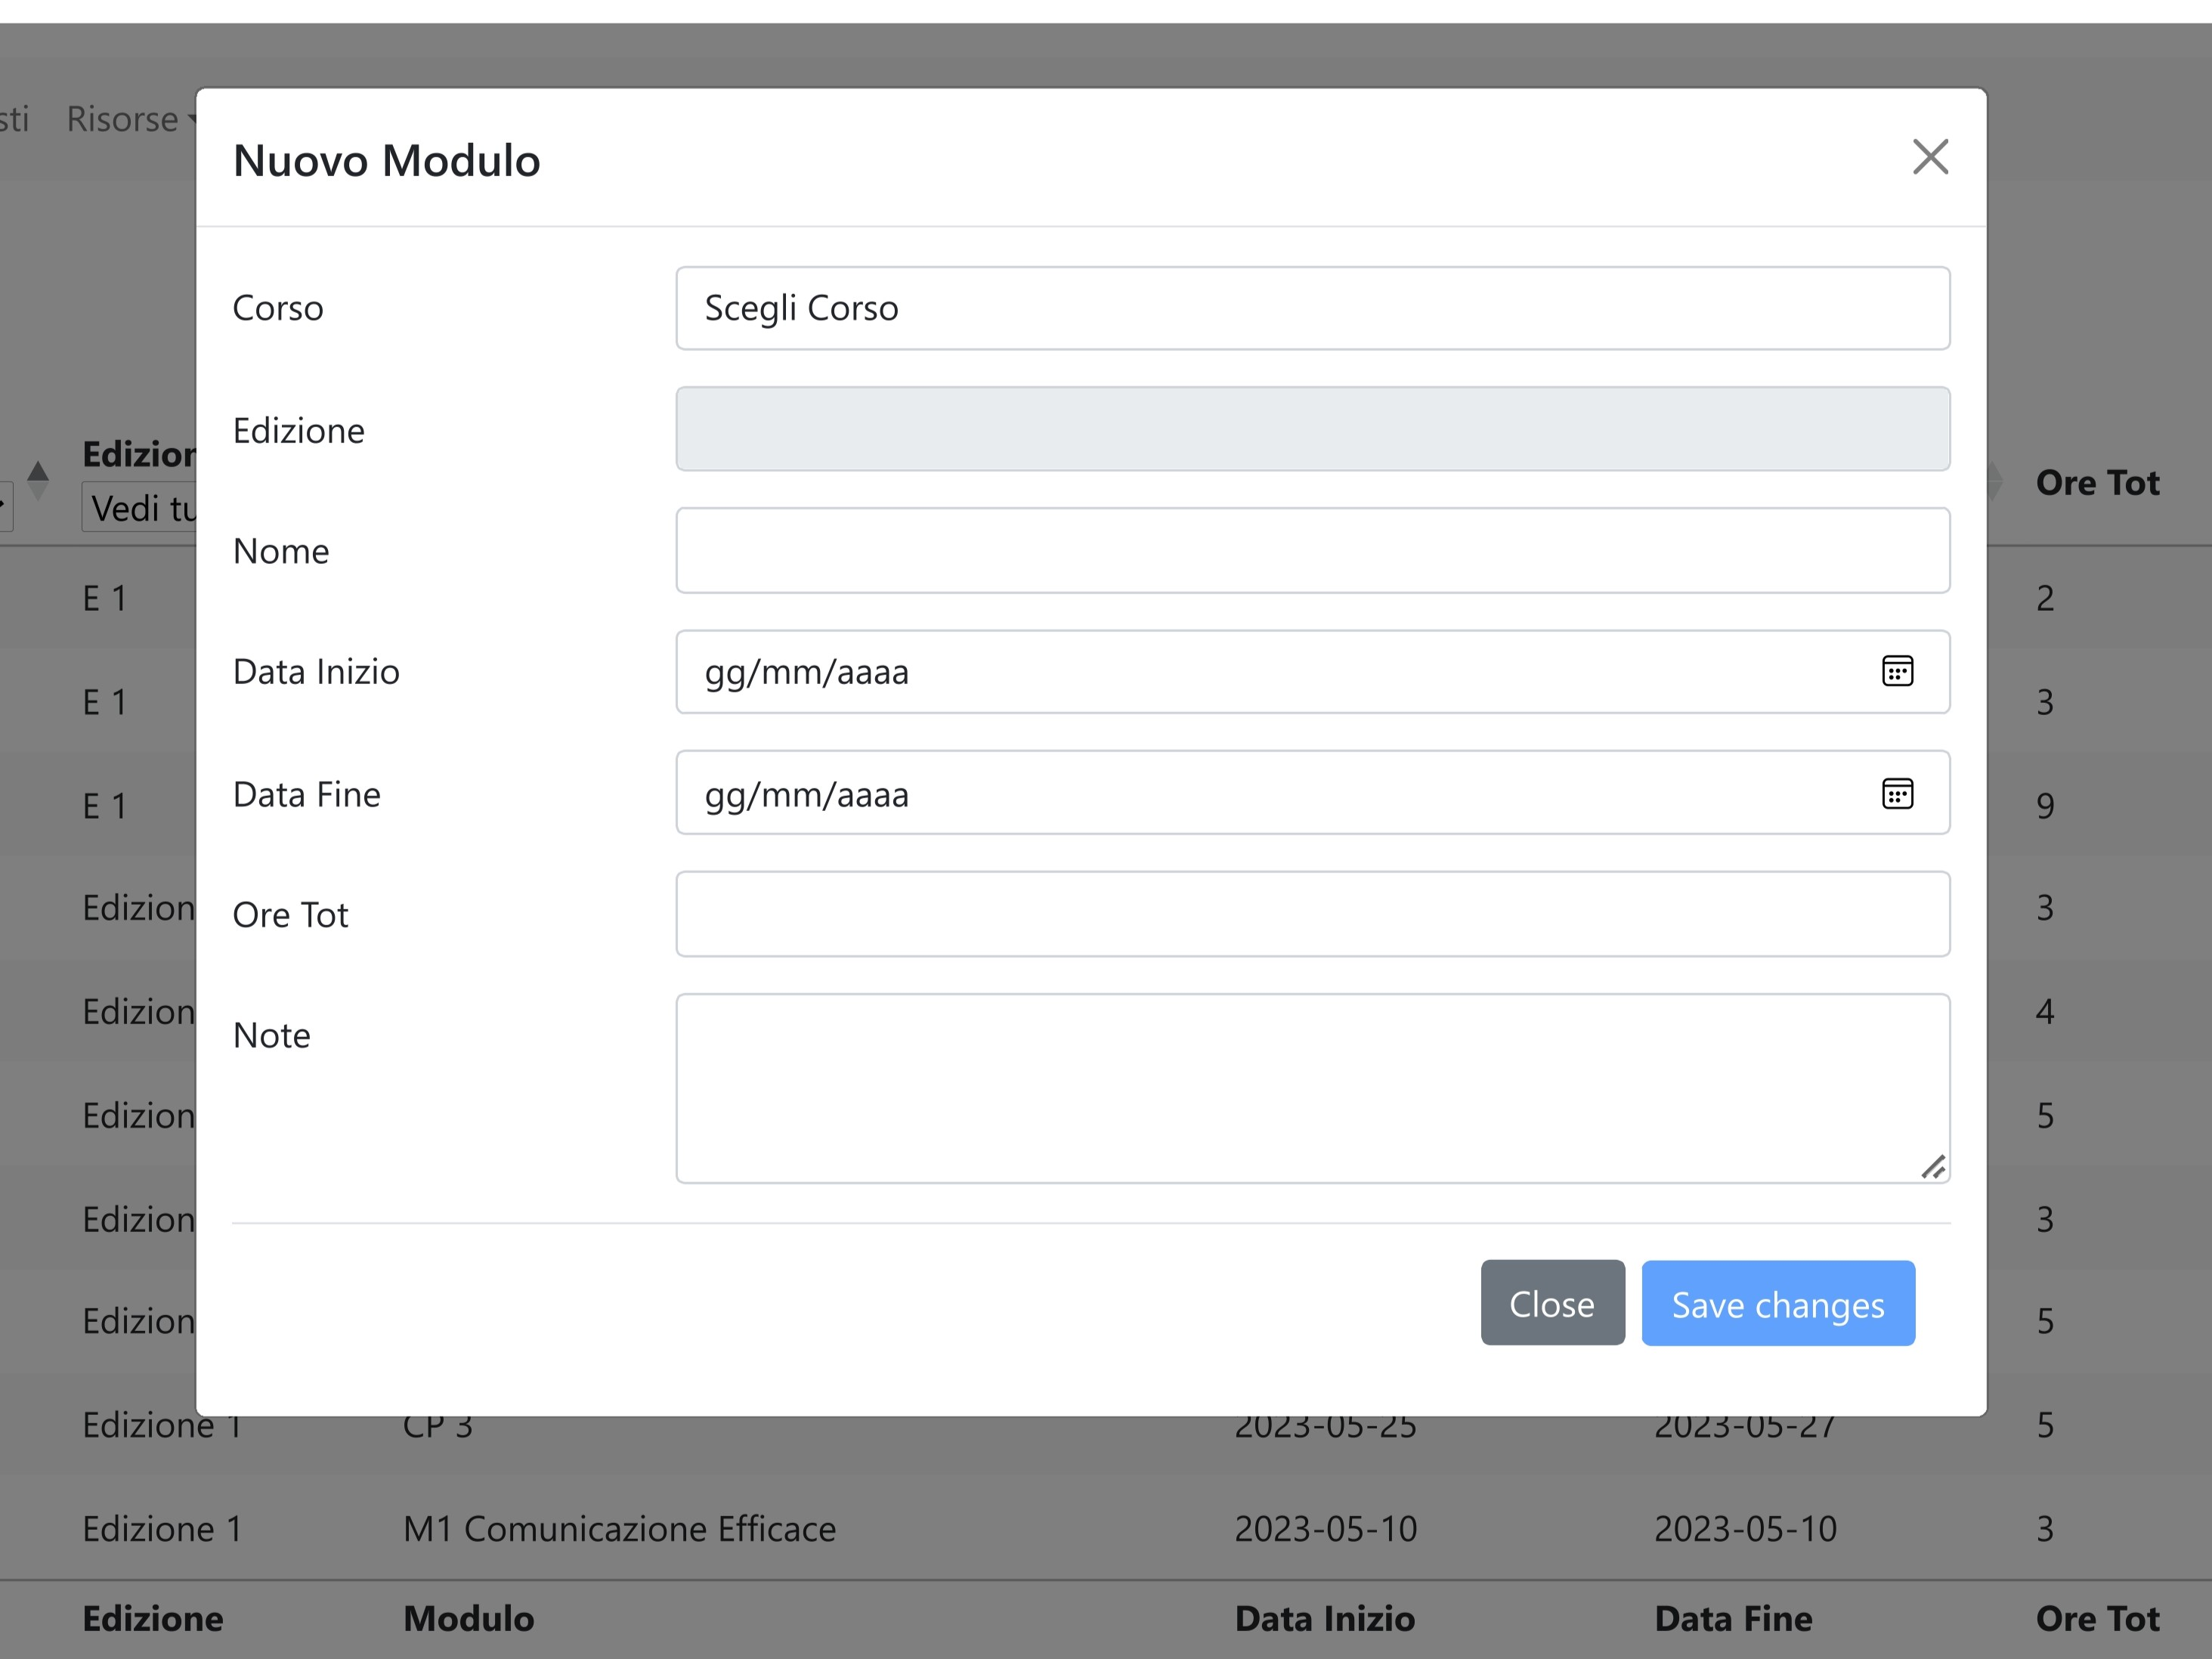
\includegraphics[width=\textwidth]{img/screen/Moduli_aggiungi-1.jpg}
     \caption{Nuovo Modulo}
     \label{fig:nuovo_modulo}
 \end{subfigure}
 \hfill
 \begin{subfigure}{0.49\textwidth}
     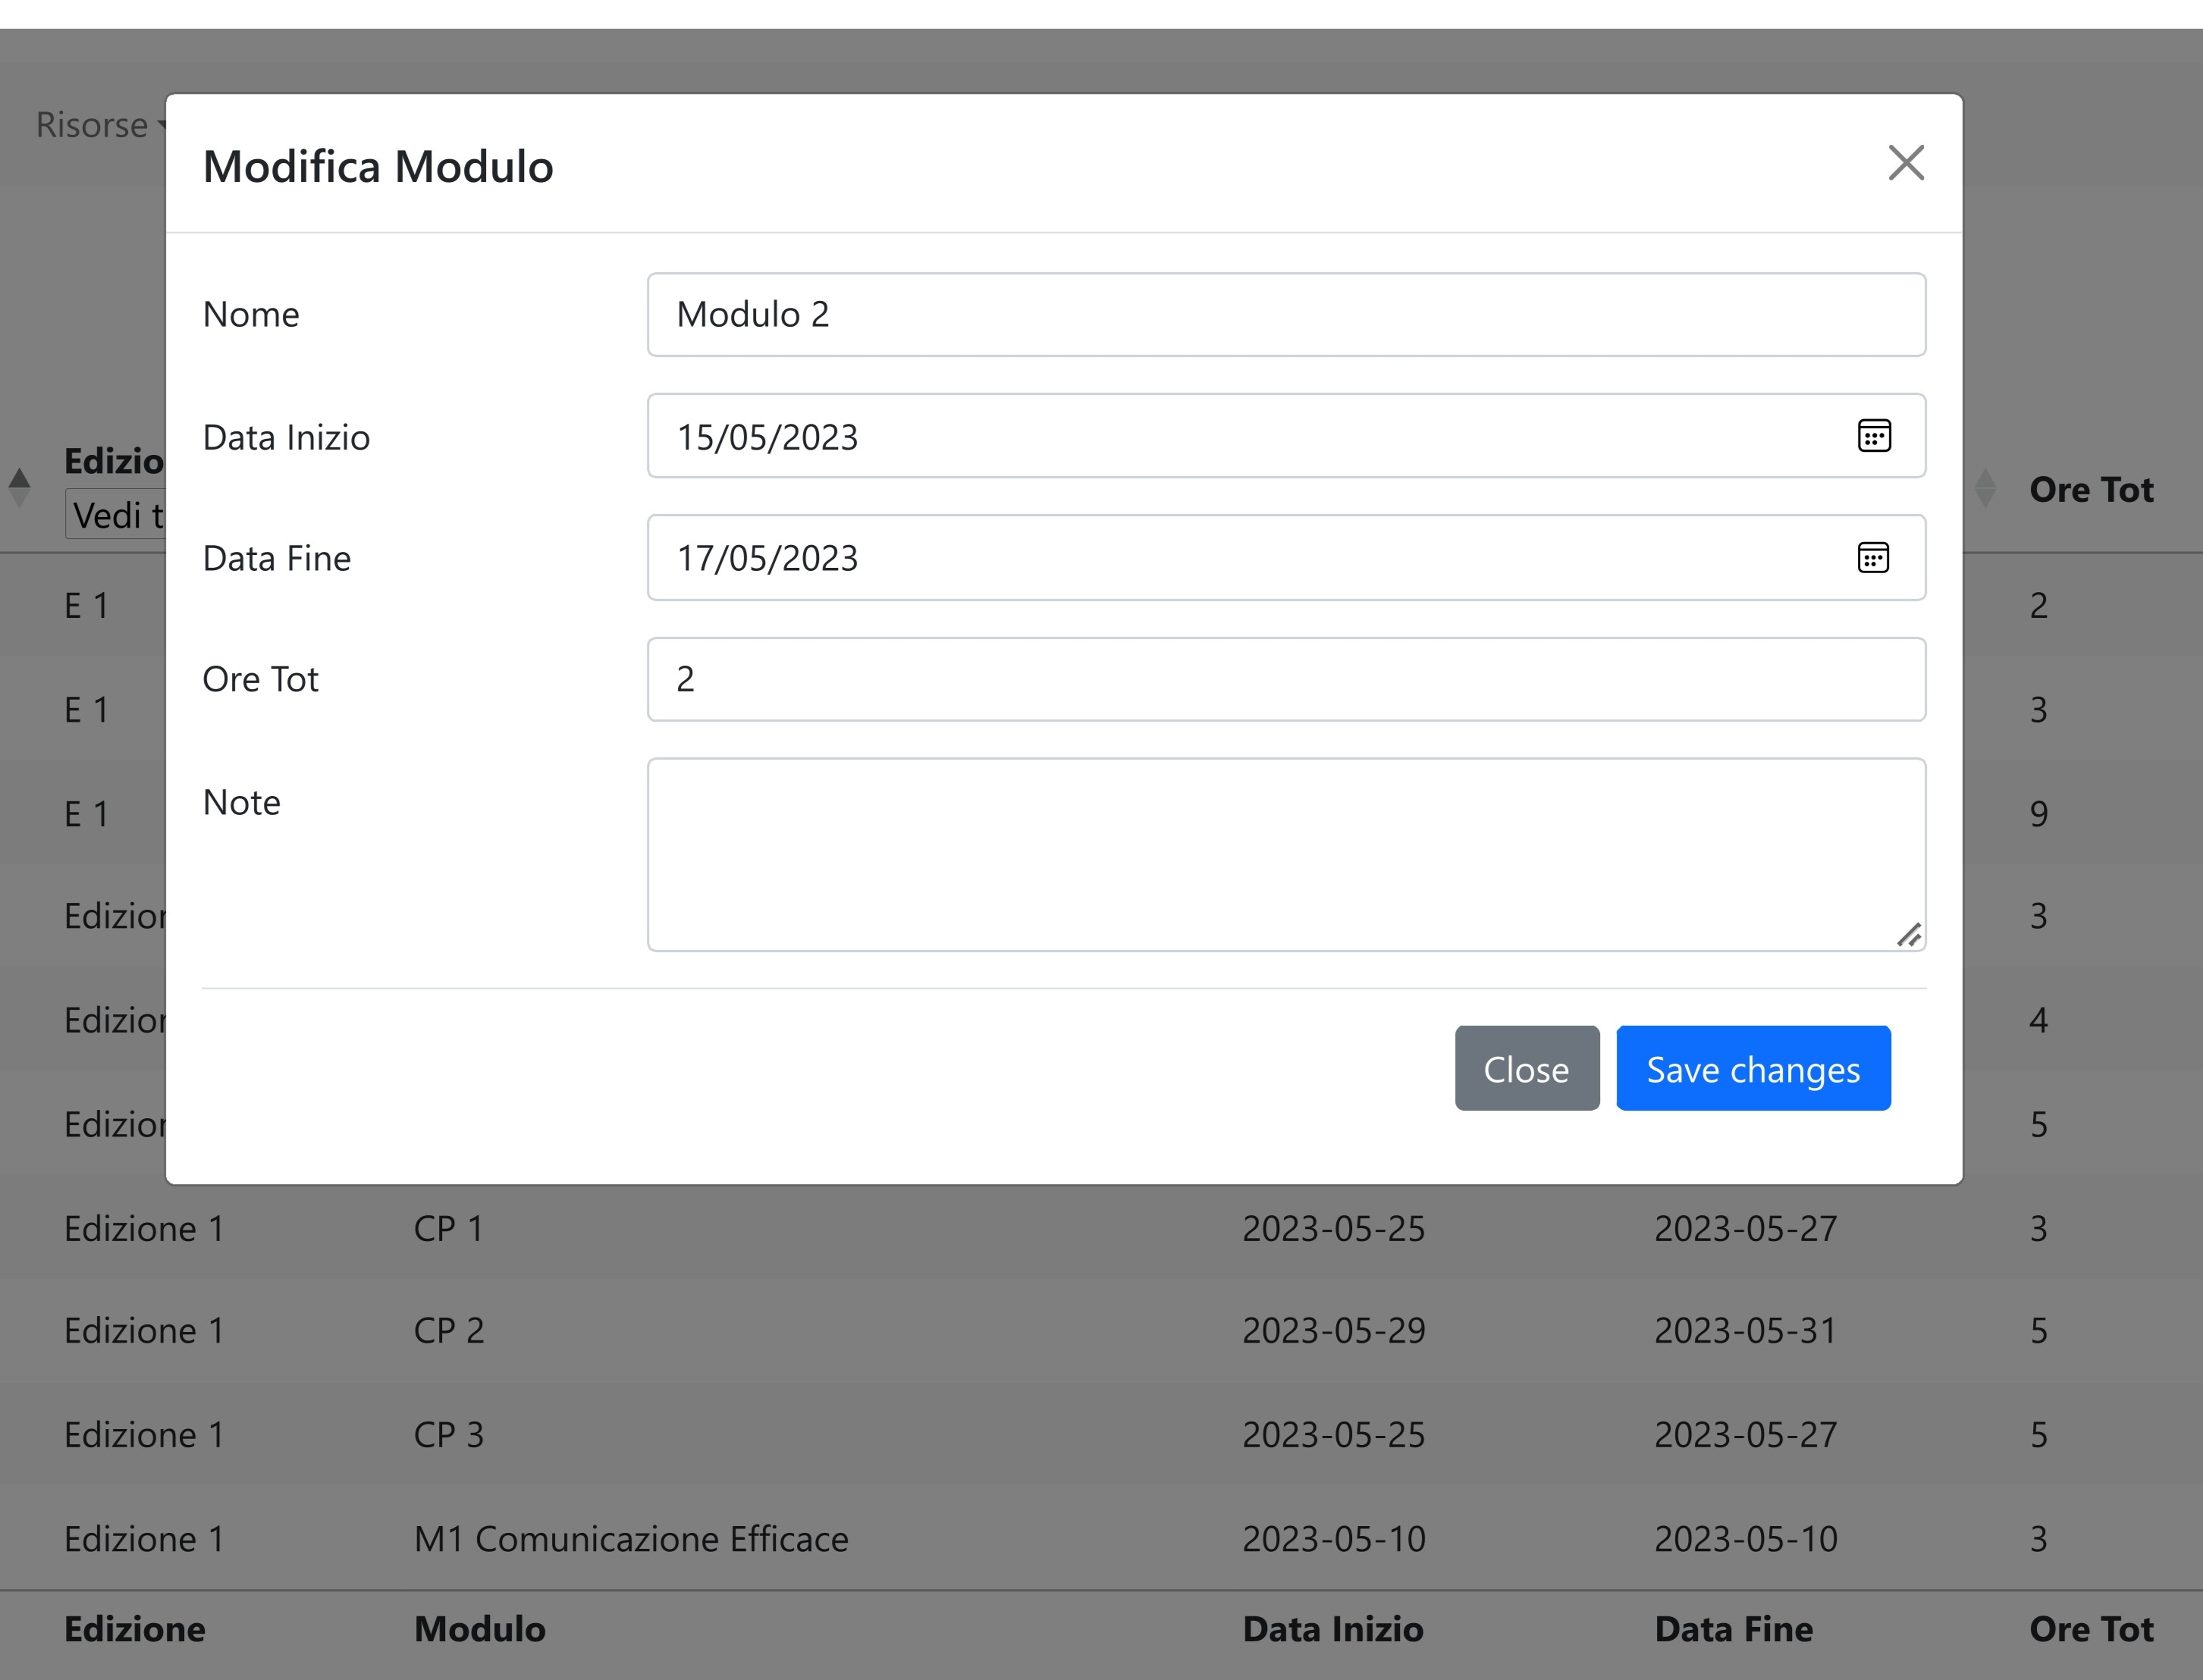
\includegraphics[width=\textwidth]{img/screen/Moduli_modifica-1.jpg}
     \caption{Modifica Modulo}
     \label{fig:modifica_modulo}
 \end{subfigure}
 %\hfill
% \begin{subfigure}{0.5\textwidth}
 %    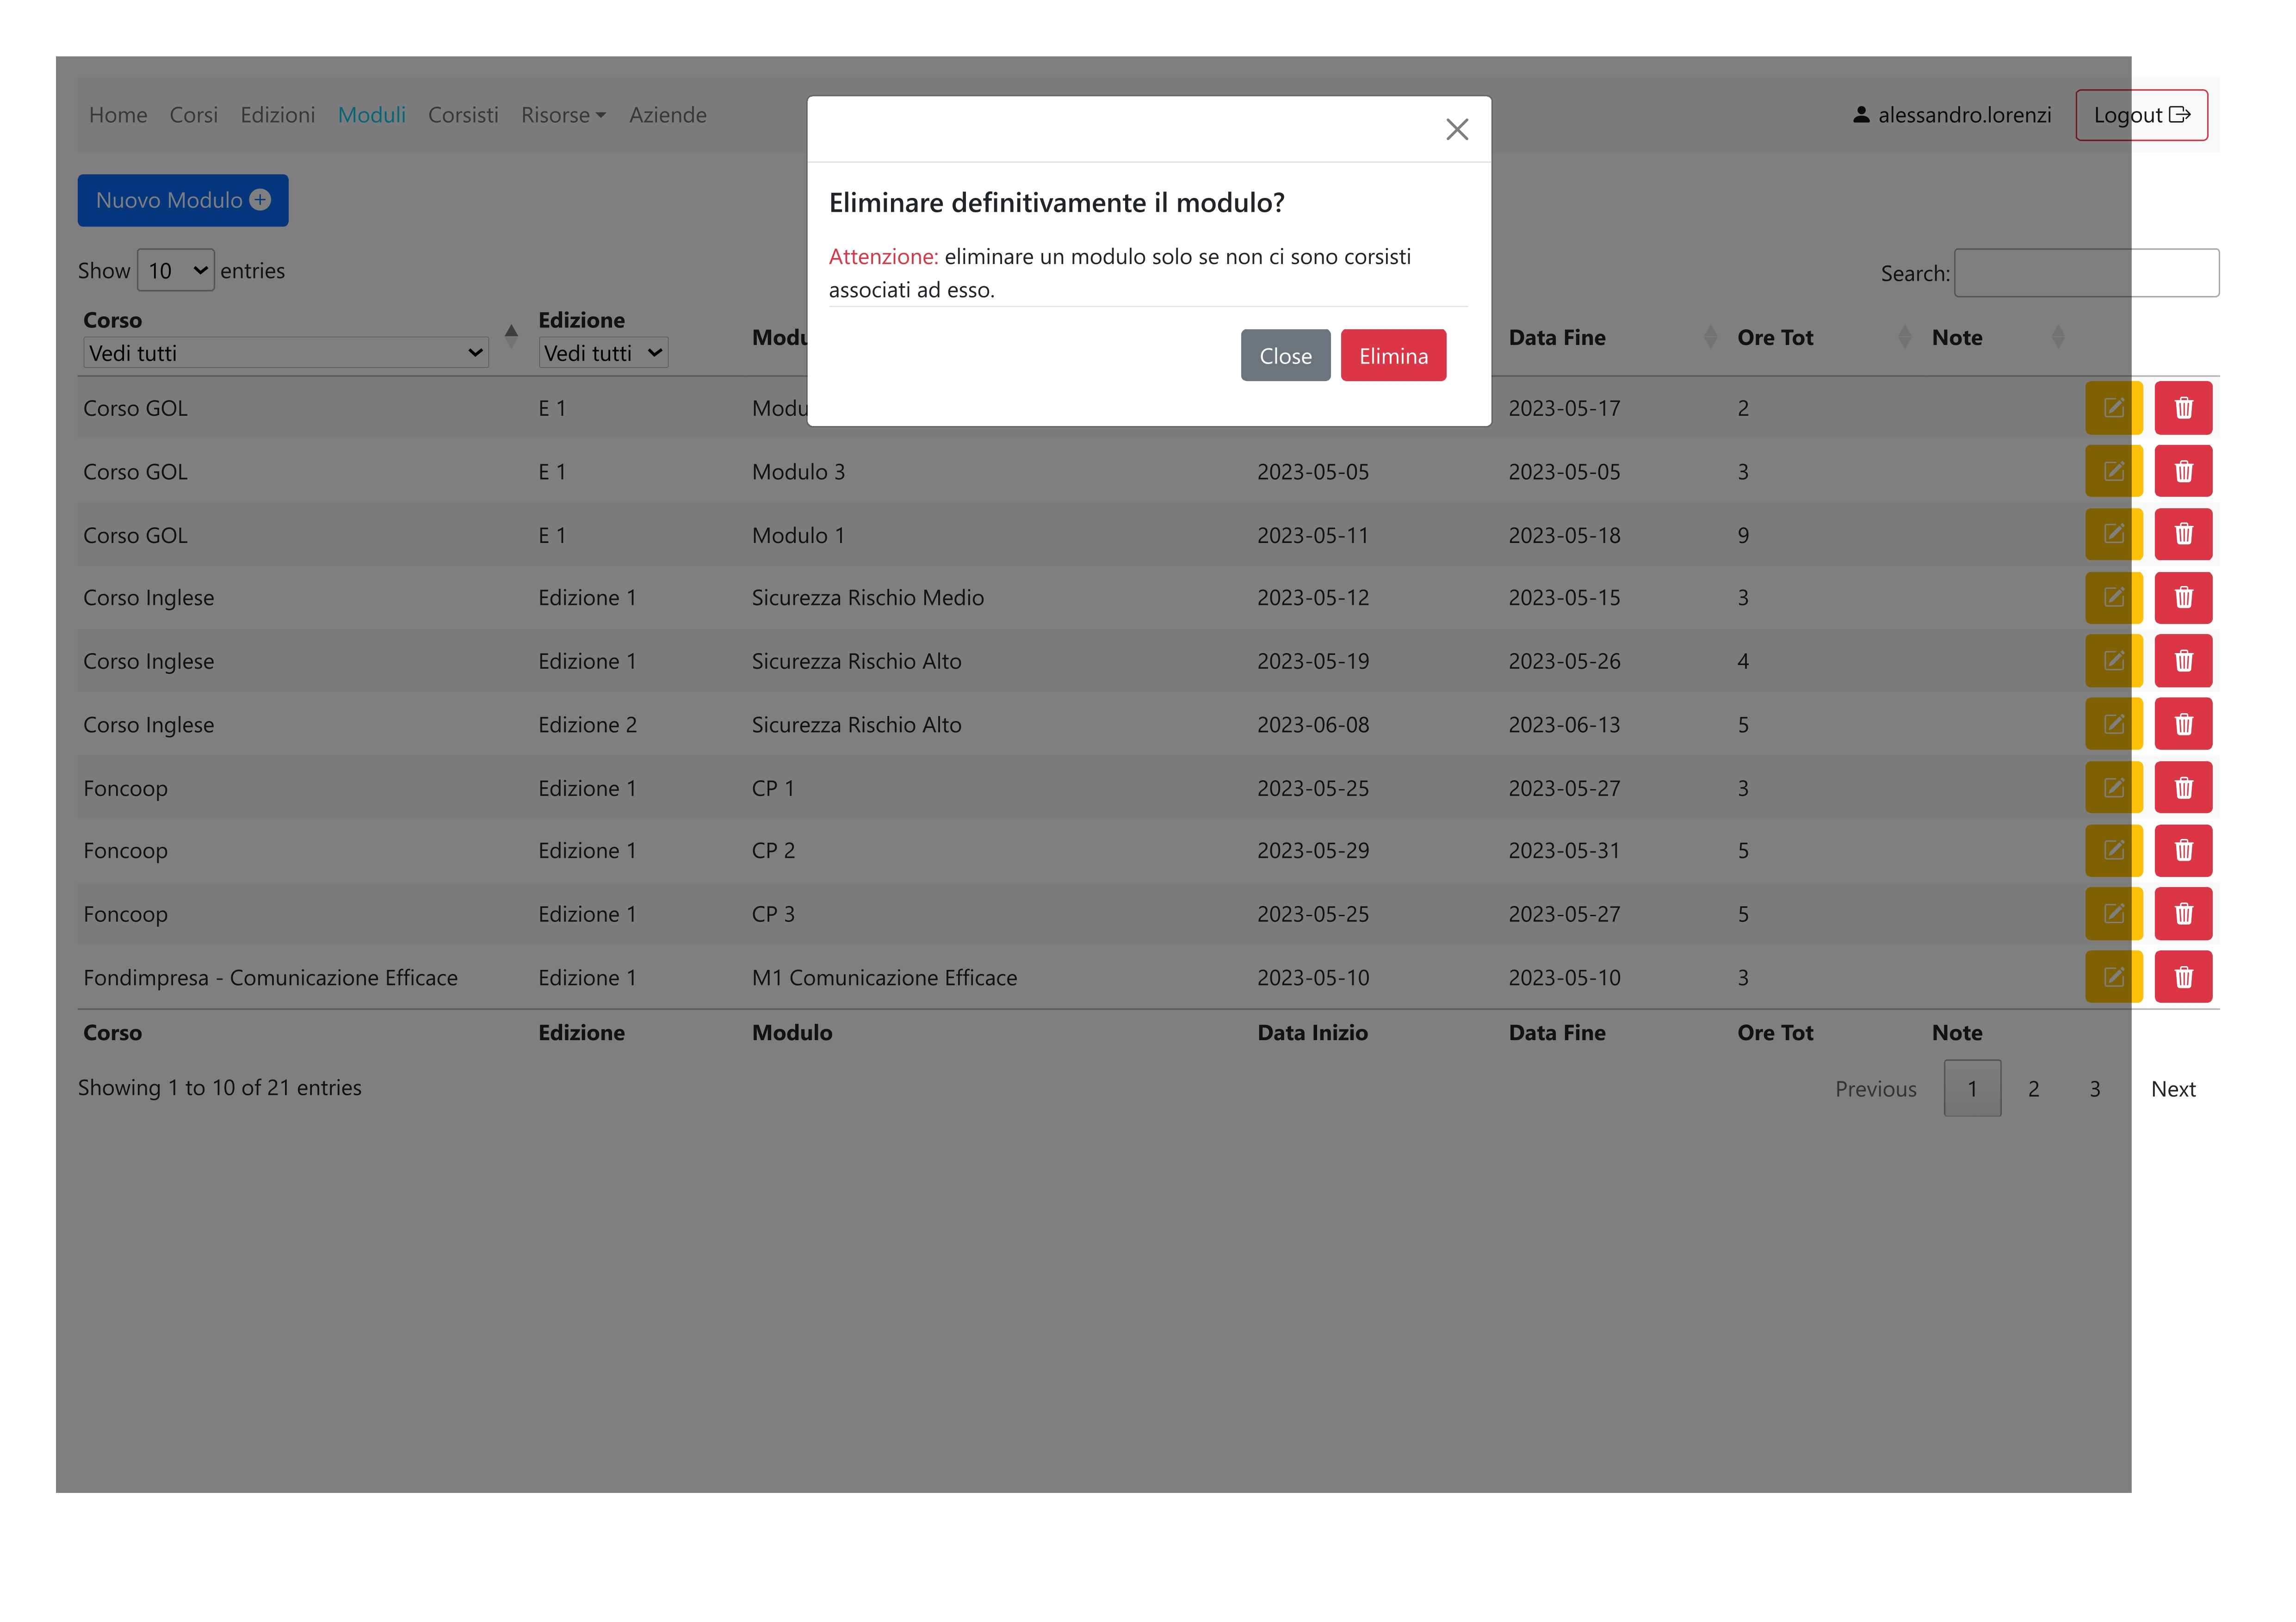
\includegraphics[width=\textwidth]{img/screen/Moduli_elimina-1.jpg}
  %   \caption{Elimina Modulo}
   %  \label{fig:elimina_modulo}
% \end{subfigure}
\caption{Operazioni sulla pagina Moduli}
\label{fig:operazioni_moduli}
\end{figure}
\newline
\section{Gestione Risorse}
Il gestionale fornisce due pagine per la gestione delle risorse e dei ruoli che queste hanno nei vari corsi: \textit{Anagrafica Risorse} e \textit{Ruoli Risorse}.
\subsection{Pagina Anagrafica Risorse}
Attraverso la pagina \textit{Anagrafica Risorse} (figura \ref{fig:risorse}) è possibile visualizzare in forma tabellare tutte le risorse, modificare o eliminare quelle già presenti o aggiungerne di nuove, nonché assegnare un ruolo a una figura specificando a quale modulo si riferisce e con che funzione. Questa sezione permette anche di vedere i documenti legati a ogni risorsa (come c.v., consensi della privacy o autorizzazioni varie). Per questa parte è stato inoltre implementato un sistema di notifiche che, al primo collegamento dell'utente, mostra quali documenti sono in scadenza (ogni tipo ha una sua scadenza).
\begin{figure}[!hbt]
\centering
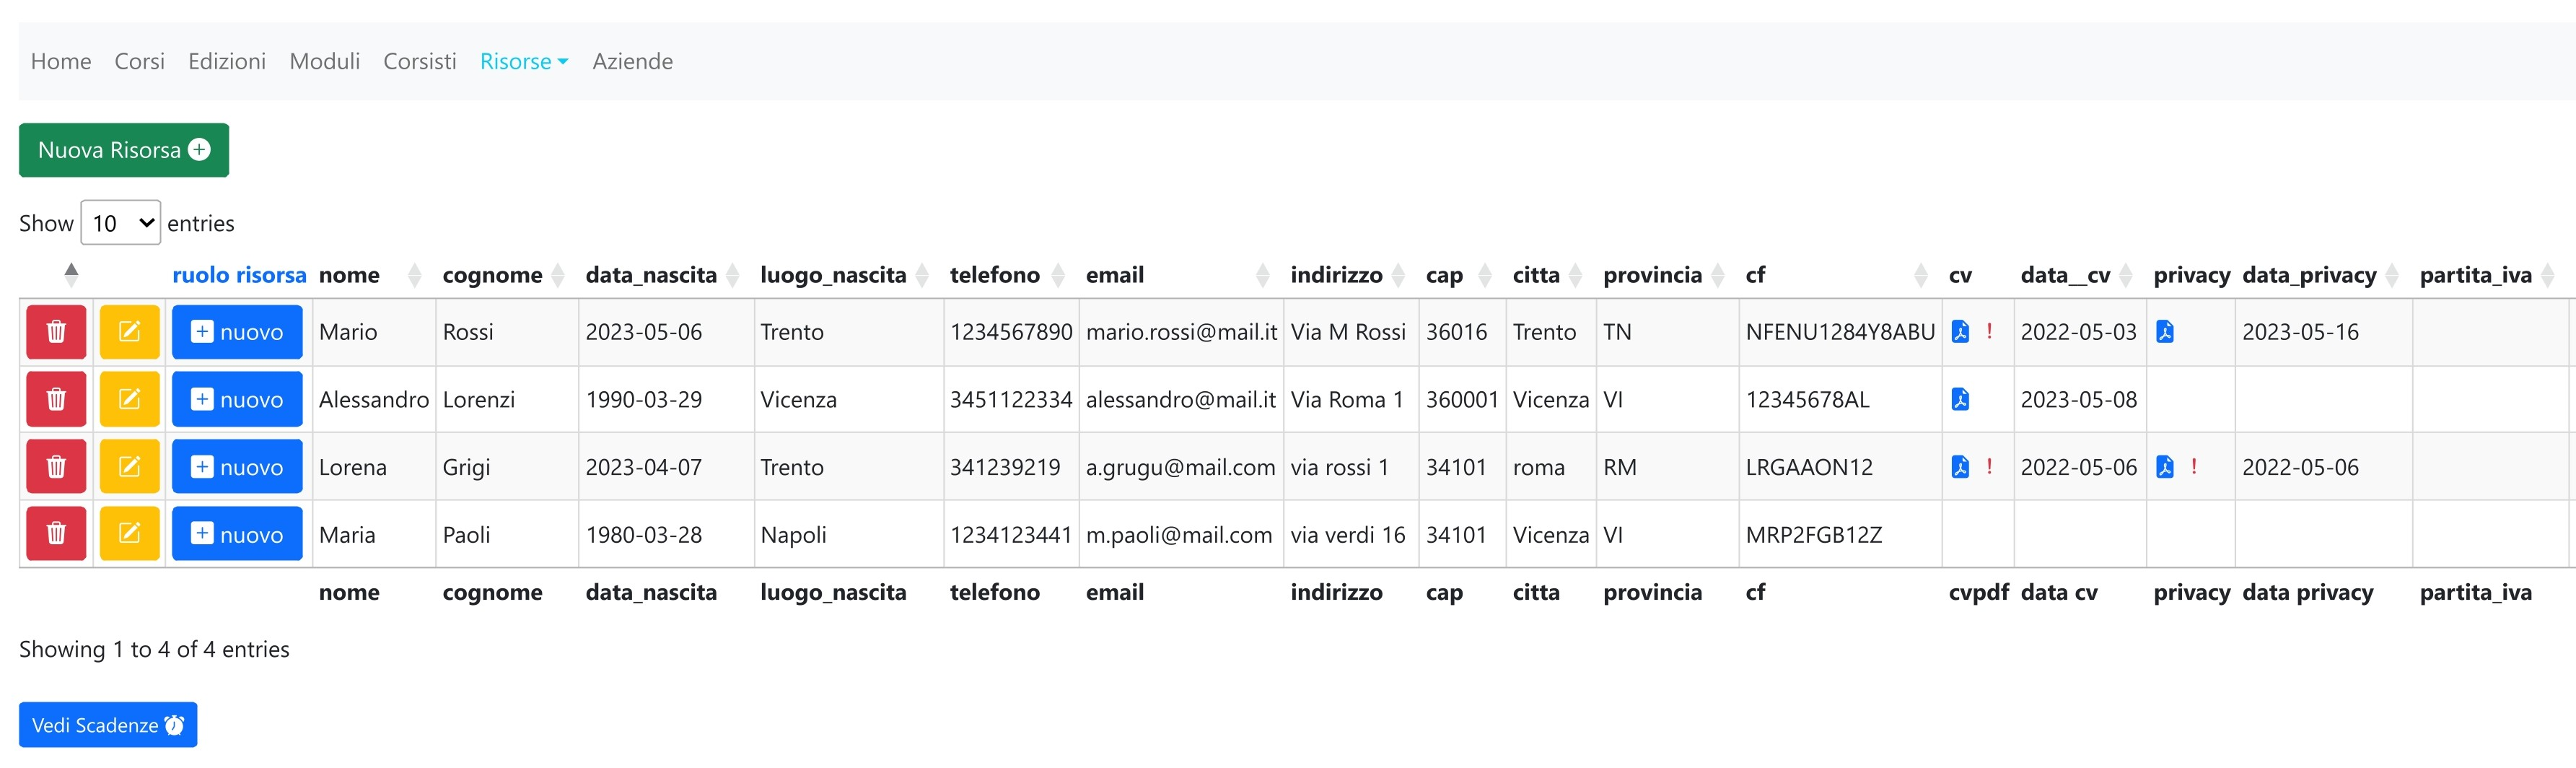
\includegraphics[scale=0.55]{img/screen/Risorse-1.jpg}
\caption{Pagina Anagrafica Risorse (screenshot)}
\label{fig:risorse}
\end{figure}
\newline
\newline
La gestione dei file PDF in un gestionale è sempre una questione delicata da trattare. In questo caso si è scelto di creare delle tabelle apposite per la memorizzazione nel database (come illustrato nello schema EER in figura \ref{fig:DiagrammaEER}), ognuna delle quali ha una struttura simile e utilizza il formato \textit{BLOB} (Binary large object) \cite{blob} per l'archiviazione di file di medie o grandi dimensioni, allocando quindi lo spazio necessario solo quando viene effettivamente utilizzato il contenuto del campo.\newline
Nel frammento di codice adattato (listing  \ref{code:blob}) si mostra come è stato gestito il caricamento di un file PDF con relativa query nel database; la parte di codice successiva (listing \ref{code:get_cv}) serve invece a restituire e mostrare il file richiesto della risorsa selezionata in modo corretto.
\begin{listing}[!hbt]
\begin{minted}{PHP}
<?php 
...
if ($_FILES['cv-risorsa']['size'] > 0) {
    $fileName = $_FILES['cv-risorsa']['name'];
    $tmpName  = $_FILES['cv-risorsa']['tmp_name'];
    $fileSize = $_FILES['cv-risorsa']['size'];
    $fileType = $_FILES['cv-risorsa']['type'];

    $fp = fopen($tmpName, 'r');
    $content = fread($fp, filesize($tmpName));
    $content = addslashes($content);
    fclose($fp);

    $fileName = addslashes($fileName);

    $query .= "SET @CVid = (SELECT LAST_INSERT_ID(pdf_cv.id_cv) from pdf_cv
    order by LAST_INSERT_ID(pdf_cv.id_cv) desc limit 1) + 1;"; //get id_cv_pdf
    $query .= "INSERT INTO pdf_cv (id_cv, filename,file_cv) " .
        "VALUES (@CVid, '$fileName', '$content');"; //insert pdf cv
    $query .= "SET @CVdate =  CURRENT_DATE;"; //set date cv
} else {
    $query .= "SET @CVid = null; SET @CVdate = null;";
}
...
\end{minted}
\caption{inserimento file BLOB in database}
\label{code:blob}
\end{listing}
\begin{listing}[!hbt]
\begin{minted}{PHP}
<?php
if (isset($_GET["id"])) {
    ...
    $id = $_GET["id"];
    if ($id != "null") {
        $query = "SELECT filename, file_cv FROM pdf_cv WHERE id_cv = '$id'";
        $result = $conn->query($query) or die($conn->error);
        $row = mysqli_fetch_assoc($result);

        header("Content-type: application/pdf");
        header('Content-disposition: inline; filename=' . $row["filename"] .
        '.pdf');
        header('Content-Transfer-Encoding: binary');
        header('Accept-Ranges: bytes');
        
        echo $row["file_cv"];
    } else {
        echo "<div>file non disponibile</div><a href='' 
        onclick='window.close()'>torna indietro</a>";
    }
    ...
}
\end{minted}
\caption{Interrogazione al database per ottenere e mostrare un file}
\label{code:get_cv}
\end{listing}

\subsection{Pagina Ruoli Risorse}
La pagina \textit{Ruoli Risorse} (figura \ref{fig:ruoli}) permette di visualizzare, filtrare e gestire le figure impegnate in uno o più moduli dei corsi presenti. Ogni risorsa può avere un ruolo diverso (docente, tutor, coordinatore, ecc.) nello stesso modulo ed essere assegnato a più moduli e corsi. Se quindi attraverso la pagina \textit{Anagrafica Risorse} è possibile effettuare l'assegnazione \textit{Risorsa-Ruolo} specificandone le informazioni necessarie, in questa pagina avviene l'amministrazione di esse.
\begin{figure}[!hbt]
\centering
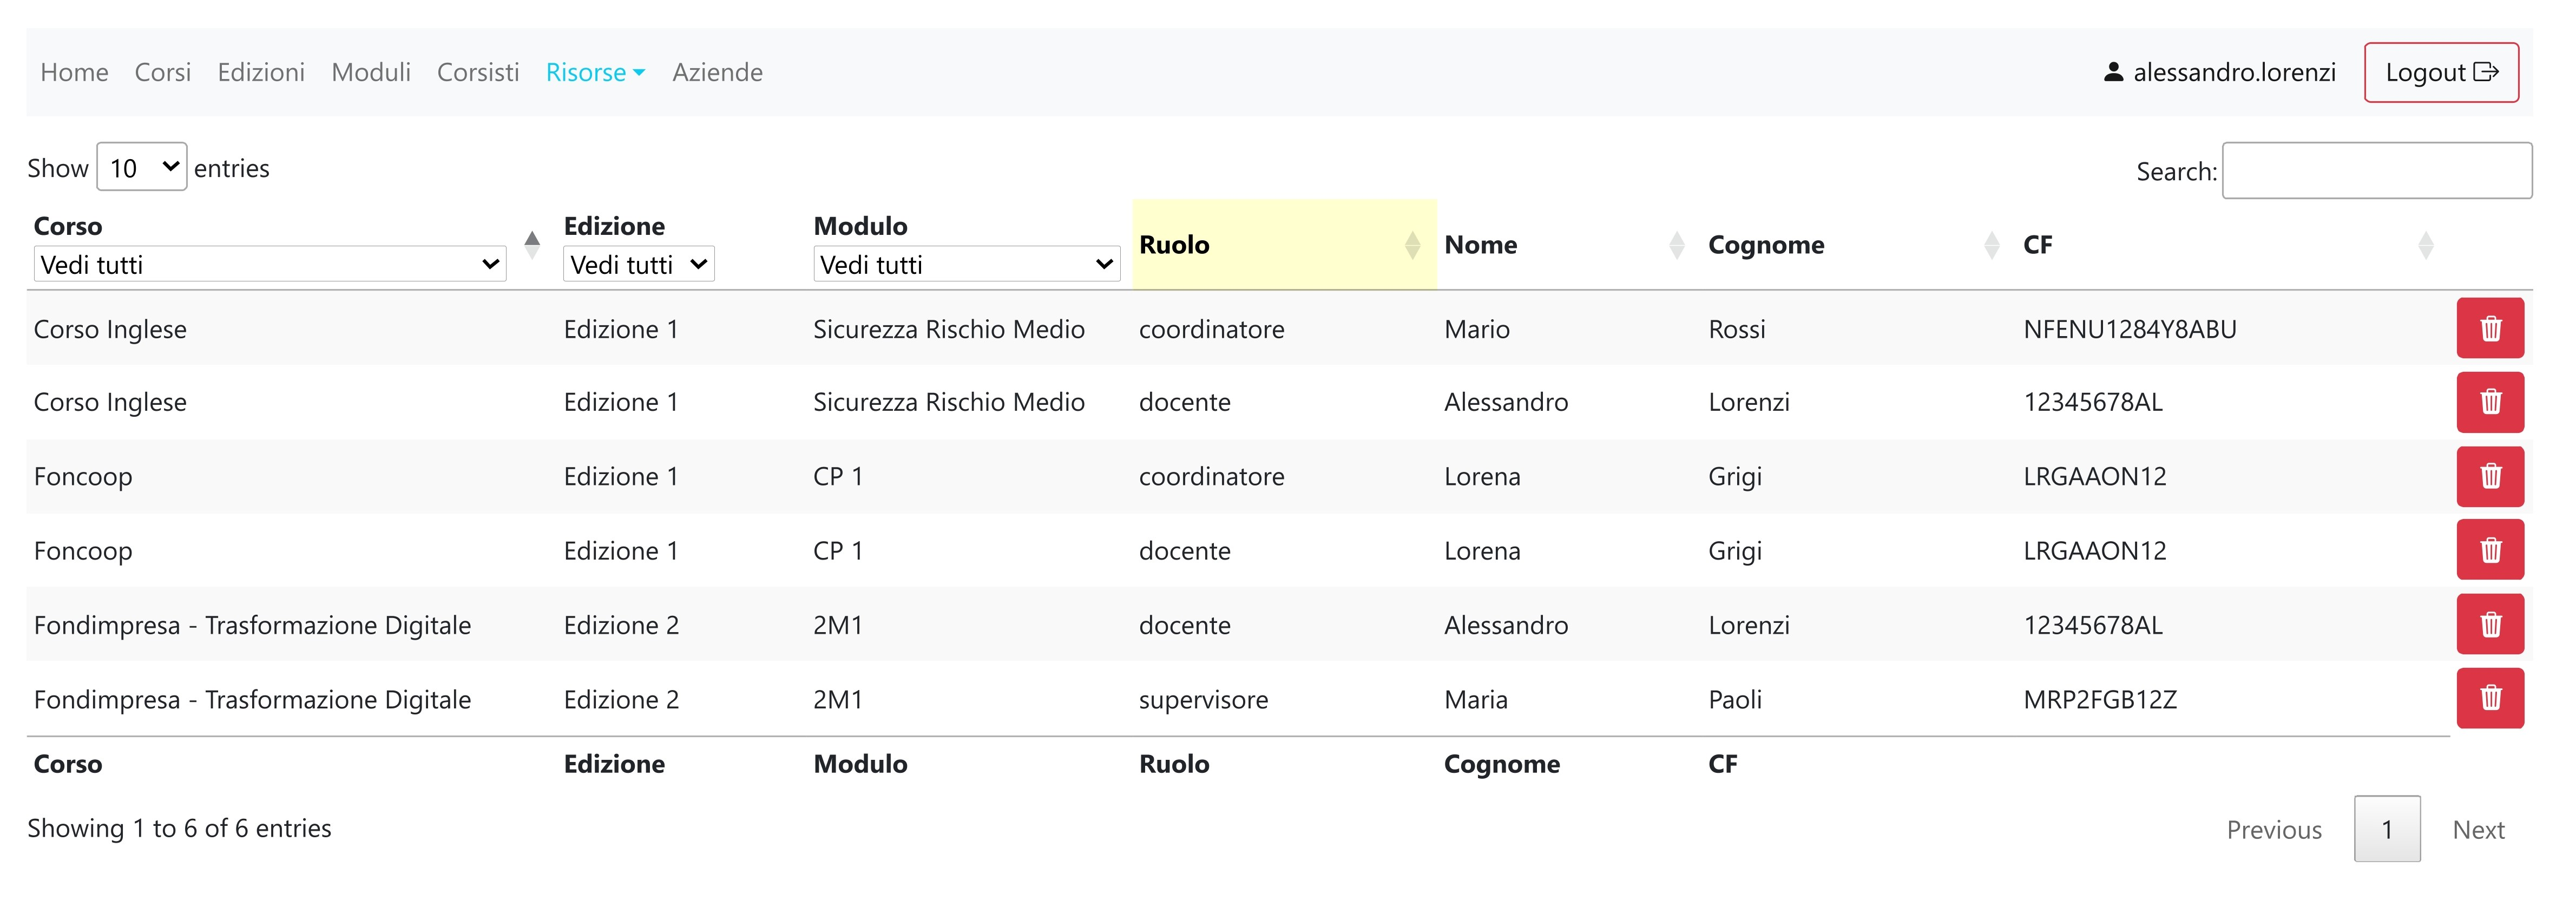
\includegraphics[scale=0.40]{img/screen/Ruoli-1.jpg}
\caption{Pagina Ruoli Risorse (screenshot)}
\label{fig:ruoli}
\end{figure}
\newline
\section{Pagina Corsisti}
La pagina \textit{Corsisti} (figura \ref{fig:corsisti}) include tutte le funzioni necessarie per la gestione di questa anagrafica. Oltre alle operazioni precedentemente descritte per le altre pagine, da quest'area l'utente può:
\begin{itemize}
  \item Scaricare gli attestati personalizzati di tutti i corsisti di un'edizione di un corso (sezione \ref{sec:attestati}).
  \item Caricare massivamente i corsisti tramite vari modelli Excel prestabiliti. Il sistema inserire quindi i dati delle nuove figure e associa ad esse tutti i moduli presenti in quell'edizione (sezione \ref{sec:excel}).
\end{itemize}
\noindent
\begin{figure}[!h]
\centering
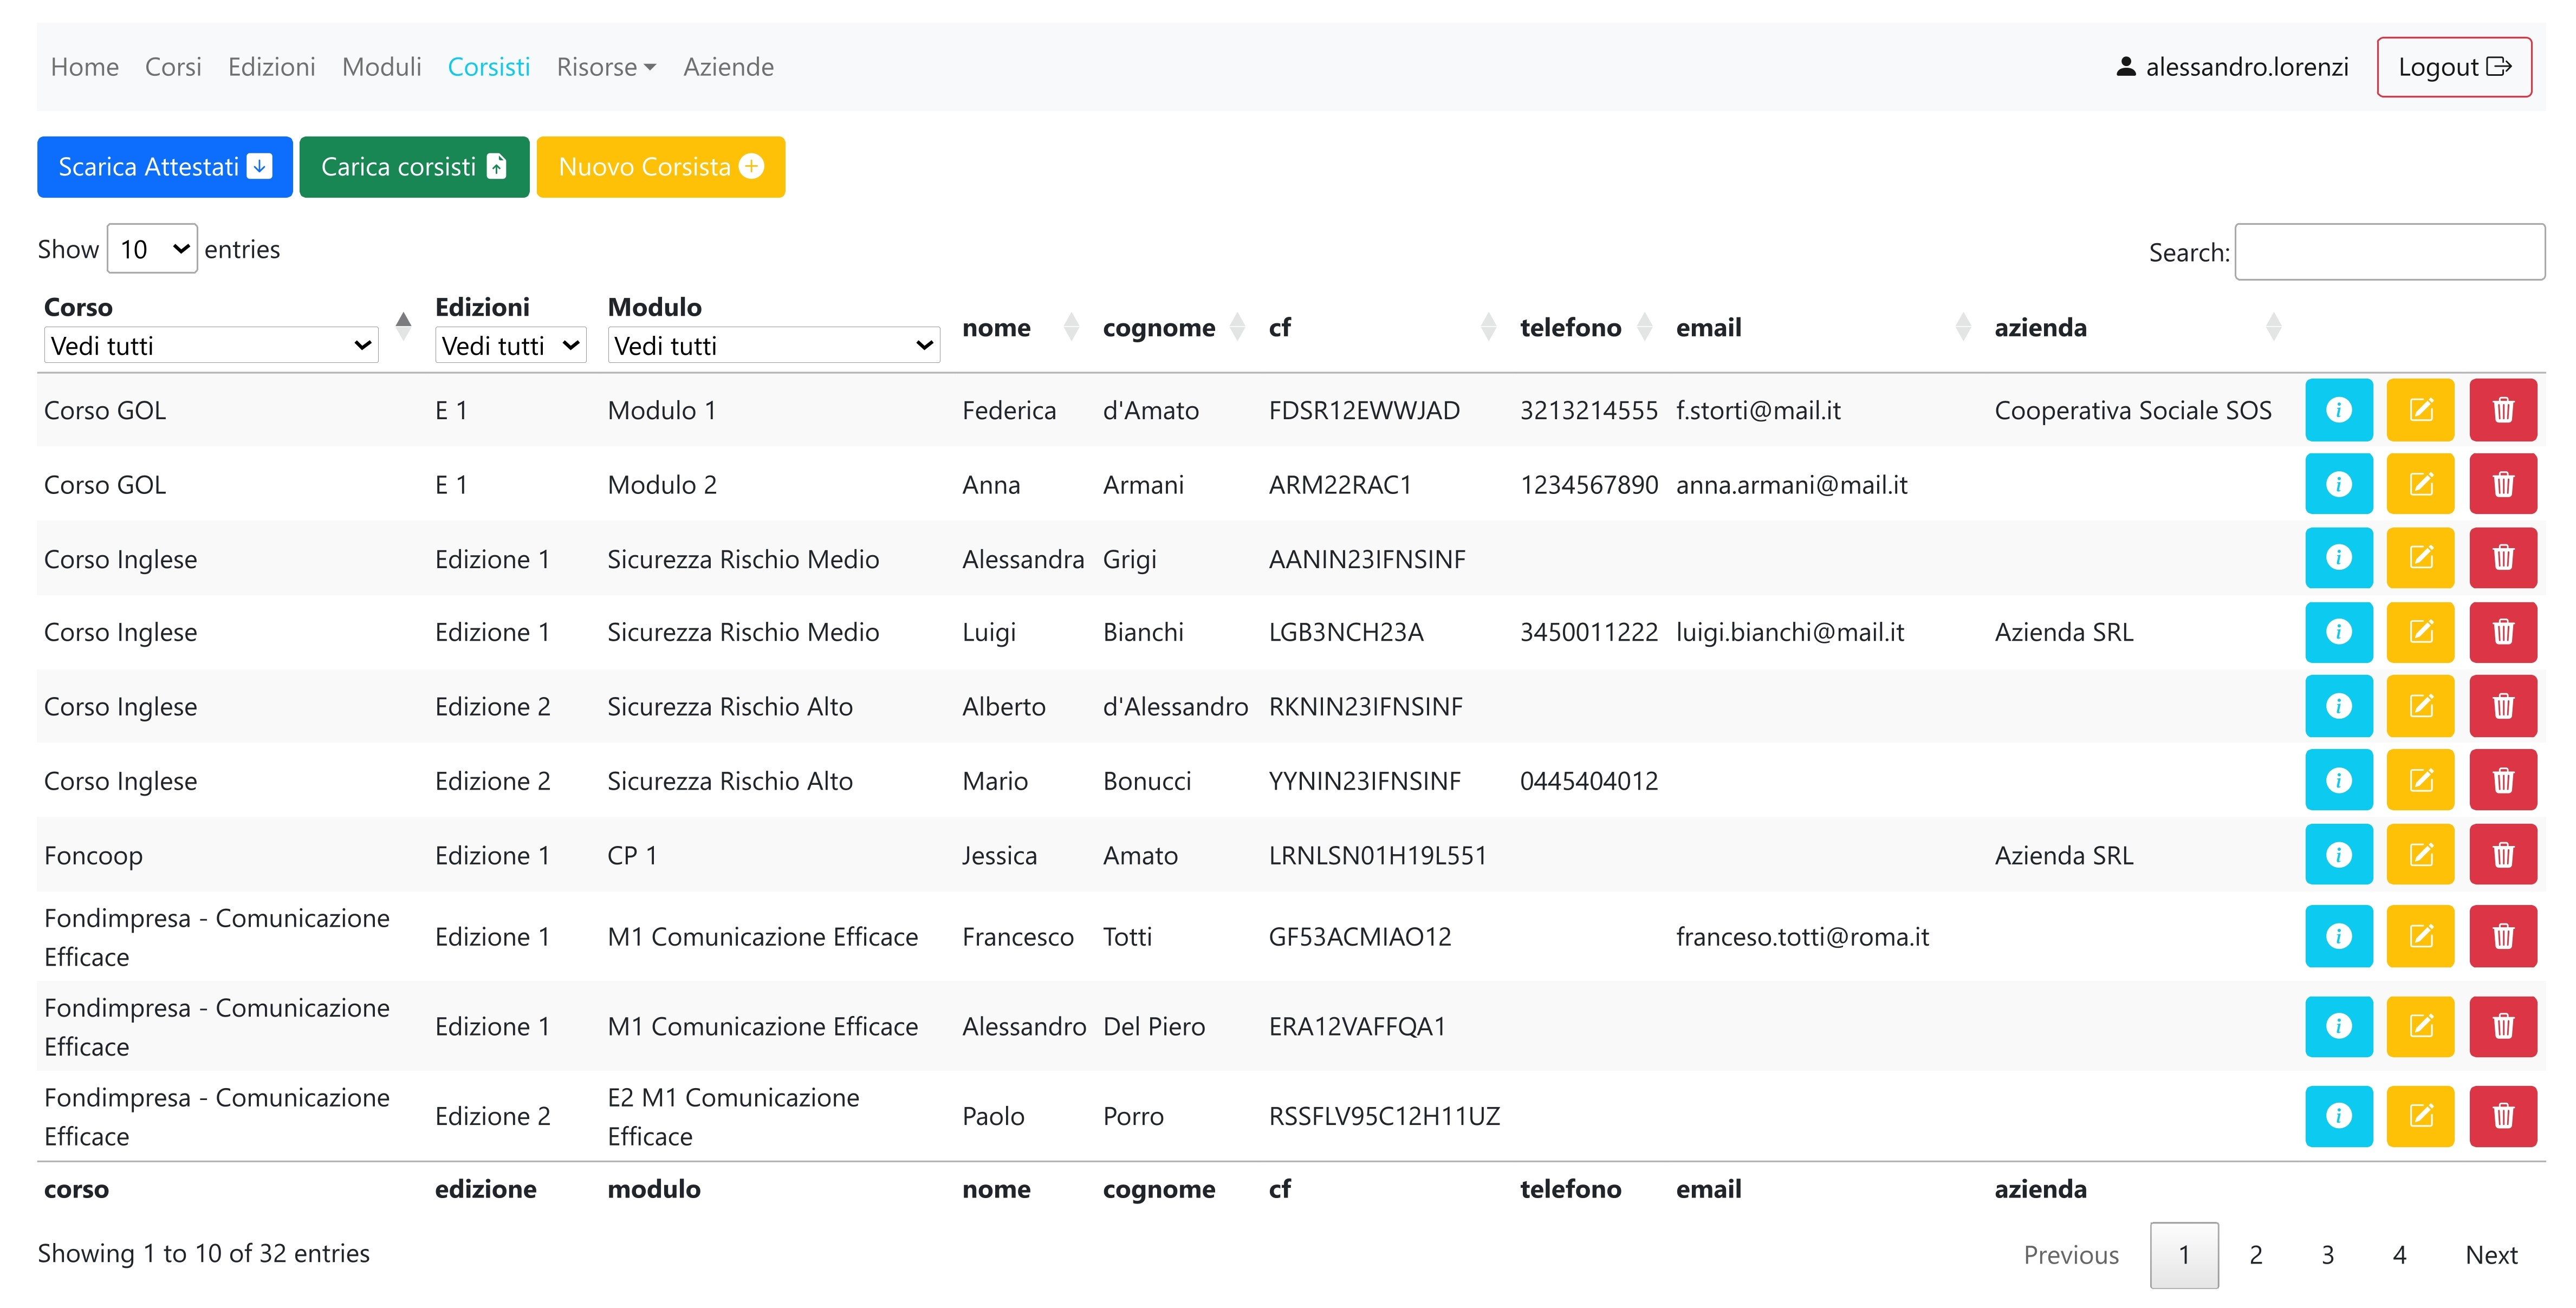
\includegraphics[scale=0.40]{img/screen/Corsisti-1.jpg}
\caption{Pagina Corsisti (screenshot)}
\label{fig:corsisti}
\end{figure}
\noindent
\subsection{Generazione di documenti}
\label{sec:attestati}
La funzione di generazione degli attestati è stata implementata usando FPDF \cite{fpdf}, classe PHP che in maniera semplice e con funzioni ad alto livello permette di generare PDF senza l'uso di altre librerie esterne più complesse e creando modelli predefiniti che vengono elaborati con dati specifici. Di seguito si riporta una frammento di codice adattato (listing \ref{code:fpdf185}) usato per generare un modello di attestato personalizzato per ogni corsista e per creare la cartella \verb|.zip| da scaricare. Il primo blocco di codice crea e riempie la cartella mentre il secondo elabora il file PDF. 
\begin{listing}[!hbt]
\begin{minted}{PHP}
<?php 
...
if ($result->num_rows > 0) {
    $zip = new ZipArchive();
    $zip->open('./test.zip', ZIPARCHIVE::OVERWRITE | ZIPARCHIVE::CREATE);
    while ($row = $result->fetch_assoc()) {
        $file = creaAttestato(... data ...);
        $zip->addFile($file);
    }
    $zip->close();
    
    $folder_path = "./";
    $files = glob($folder_path . '/*.pdf');
    foreach ($files as $file) {
        if (is_file($file)) {
            unlink($file);
        }
    }
    ...
}

...
function creaAttestato(... data ...)
{
    $pdf = new FPDF('P', 'mm', 'A4');
    $pdf->AddPage();
    $pdf->SetFont('Arial', 'I', 7);

    //write pdf ...
    
    $file = trim($nome) . '_' . trim($cognome) . '.pdf';
    trim($nome) . '_' . trim($cognome) . '.pdf';
    $pdf->Output($file, 'F');
    return $file;
}
\end{minted}
\caption{fpdf185 in PHP}
\label{code:fpdf185}
\end{listing}
\noindent
\newline

\subsection{Gestione di fogli elettronici}
\label{sec:excel}
Per la lettura dei dati dai fogli elettronici è stata scelta la classe SimpleXLSX \cite{simpleXLSX} che, senza estensioni aggiuntive, analizza, recupera ed effettua il parsing dei dati dai file Excel. Lo script di codice adattato riportato (listing \ref{code:simpleXLSX}) mostra la lettura dei dati da file \verb|.xlsx| a cui poi seguirà l'importazione a database.
\begin{listing}[!hbt]
\begin{minted}{PHP}

<?php 
...
use Shuchkin\SimpleXLSX;
ini_set('error_reporting', E_ALL);
ini_set('display_errors', true);
if ($xlsx = SimpleXLSX::parse($_FILES['file']['tmp_name'])){
    ...
    $dim = $xlsx->dimension();
    $cols = $dim[0];
    foreach ($xlsx->readRows() as $k => $r) {
        if ($k < 4) continue; // skip firsts 4 rows

            if ($r[10] != "") { //stop
                if ($r[18] != '') //check if "azienda" is NULL
                    $query = "INSERT INTO corsista (id_corsista, nome, cognome,
                    data_nascita, luogo_nascita, sesso, cf, telefono, email,
                    indirizzo, cap, citta, provincia, cittadinanza, titolo_studio,
                    categoria, intestatario_cc, coordinate_cc, tipo_contratto,
                    data_assunzione, note, azienda_cf, inquadramento) VALUES 
                    (NULL,'$r[1]', '$r[0]', '$r[2]', '$r[6]', '$r[3]', '$r[10]',NULL,
                    NULL, NULL, NULL, NULL, NULL, '$r[7]', '$r[11]', NULL, NULL, NULL,
                    '$r[12]', '$r[16]', NULL, '$r[18]', '$r[15]');";


                //get id_corsista
                $query .= "SET @CorsistaID = (SELECT LAST_INSERT_ID(
                corsista.id_corsista) from corsista order by LAST_INSERT_ID(
                corsista.id_corsista) desc limit 1);";

                //insert corso - edizione
                $query .= "INSERT INTO corsista_modulo SELECT NULL, @CorsistaID,
                m.id_modulo, 1 FROM modulo m INNER JOIN edizione e on m.edizione
                = e.id_edizione INNER JOIN corso co on e.corso = co.id_corso 
                WHERE co.id_corso = '$corso' AND e.id_edizione = '$edizione'";

                //run multi_query
                $conn->multi_query($query);
                while (mysqli_more_results($conn)) {
                    mysqli_next_result($conn);
                }
                if ($conn->multi_query($query) == FALSE) {
                    echo "Error: " . $query . "<br>" . $conn->error;
                }
            }
        }
    }
} else {
    echo SimpleXLSX::parseError();
}
\end{minted}
\caption{SimpleXLSX in PHP}
\label{code:simpleXLSX}
\end{listing}
\section{Pagina Pubblica}
Un'altra richiesta implementata è stata quella di avere una pagina pubblica raggiungibile da possibili docenti esterni che, completando un modulo di registrazione, vengono inseriti a sistema e quindi mostrati nella pagina delle risorse per poi potenzialmente essere associati a un ruolo. In figura \ref{fig:public} si mostra la pagina pubblica menzionata. Questo modulo è l'unico che non richiede l'accesso con credenziali. Il gestionale effettua una serie di controlli di correttezza dei dati compilati prima di procedere con l'effettiva memorizzazione nel database. 
\begin{figure}[!hbt]
\centering
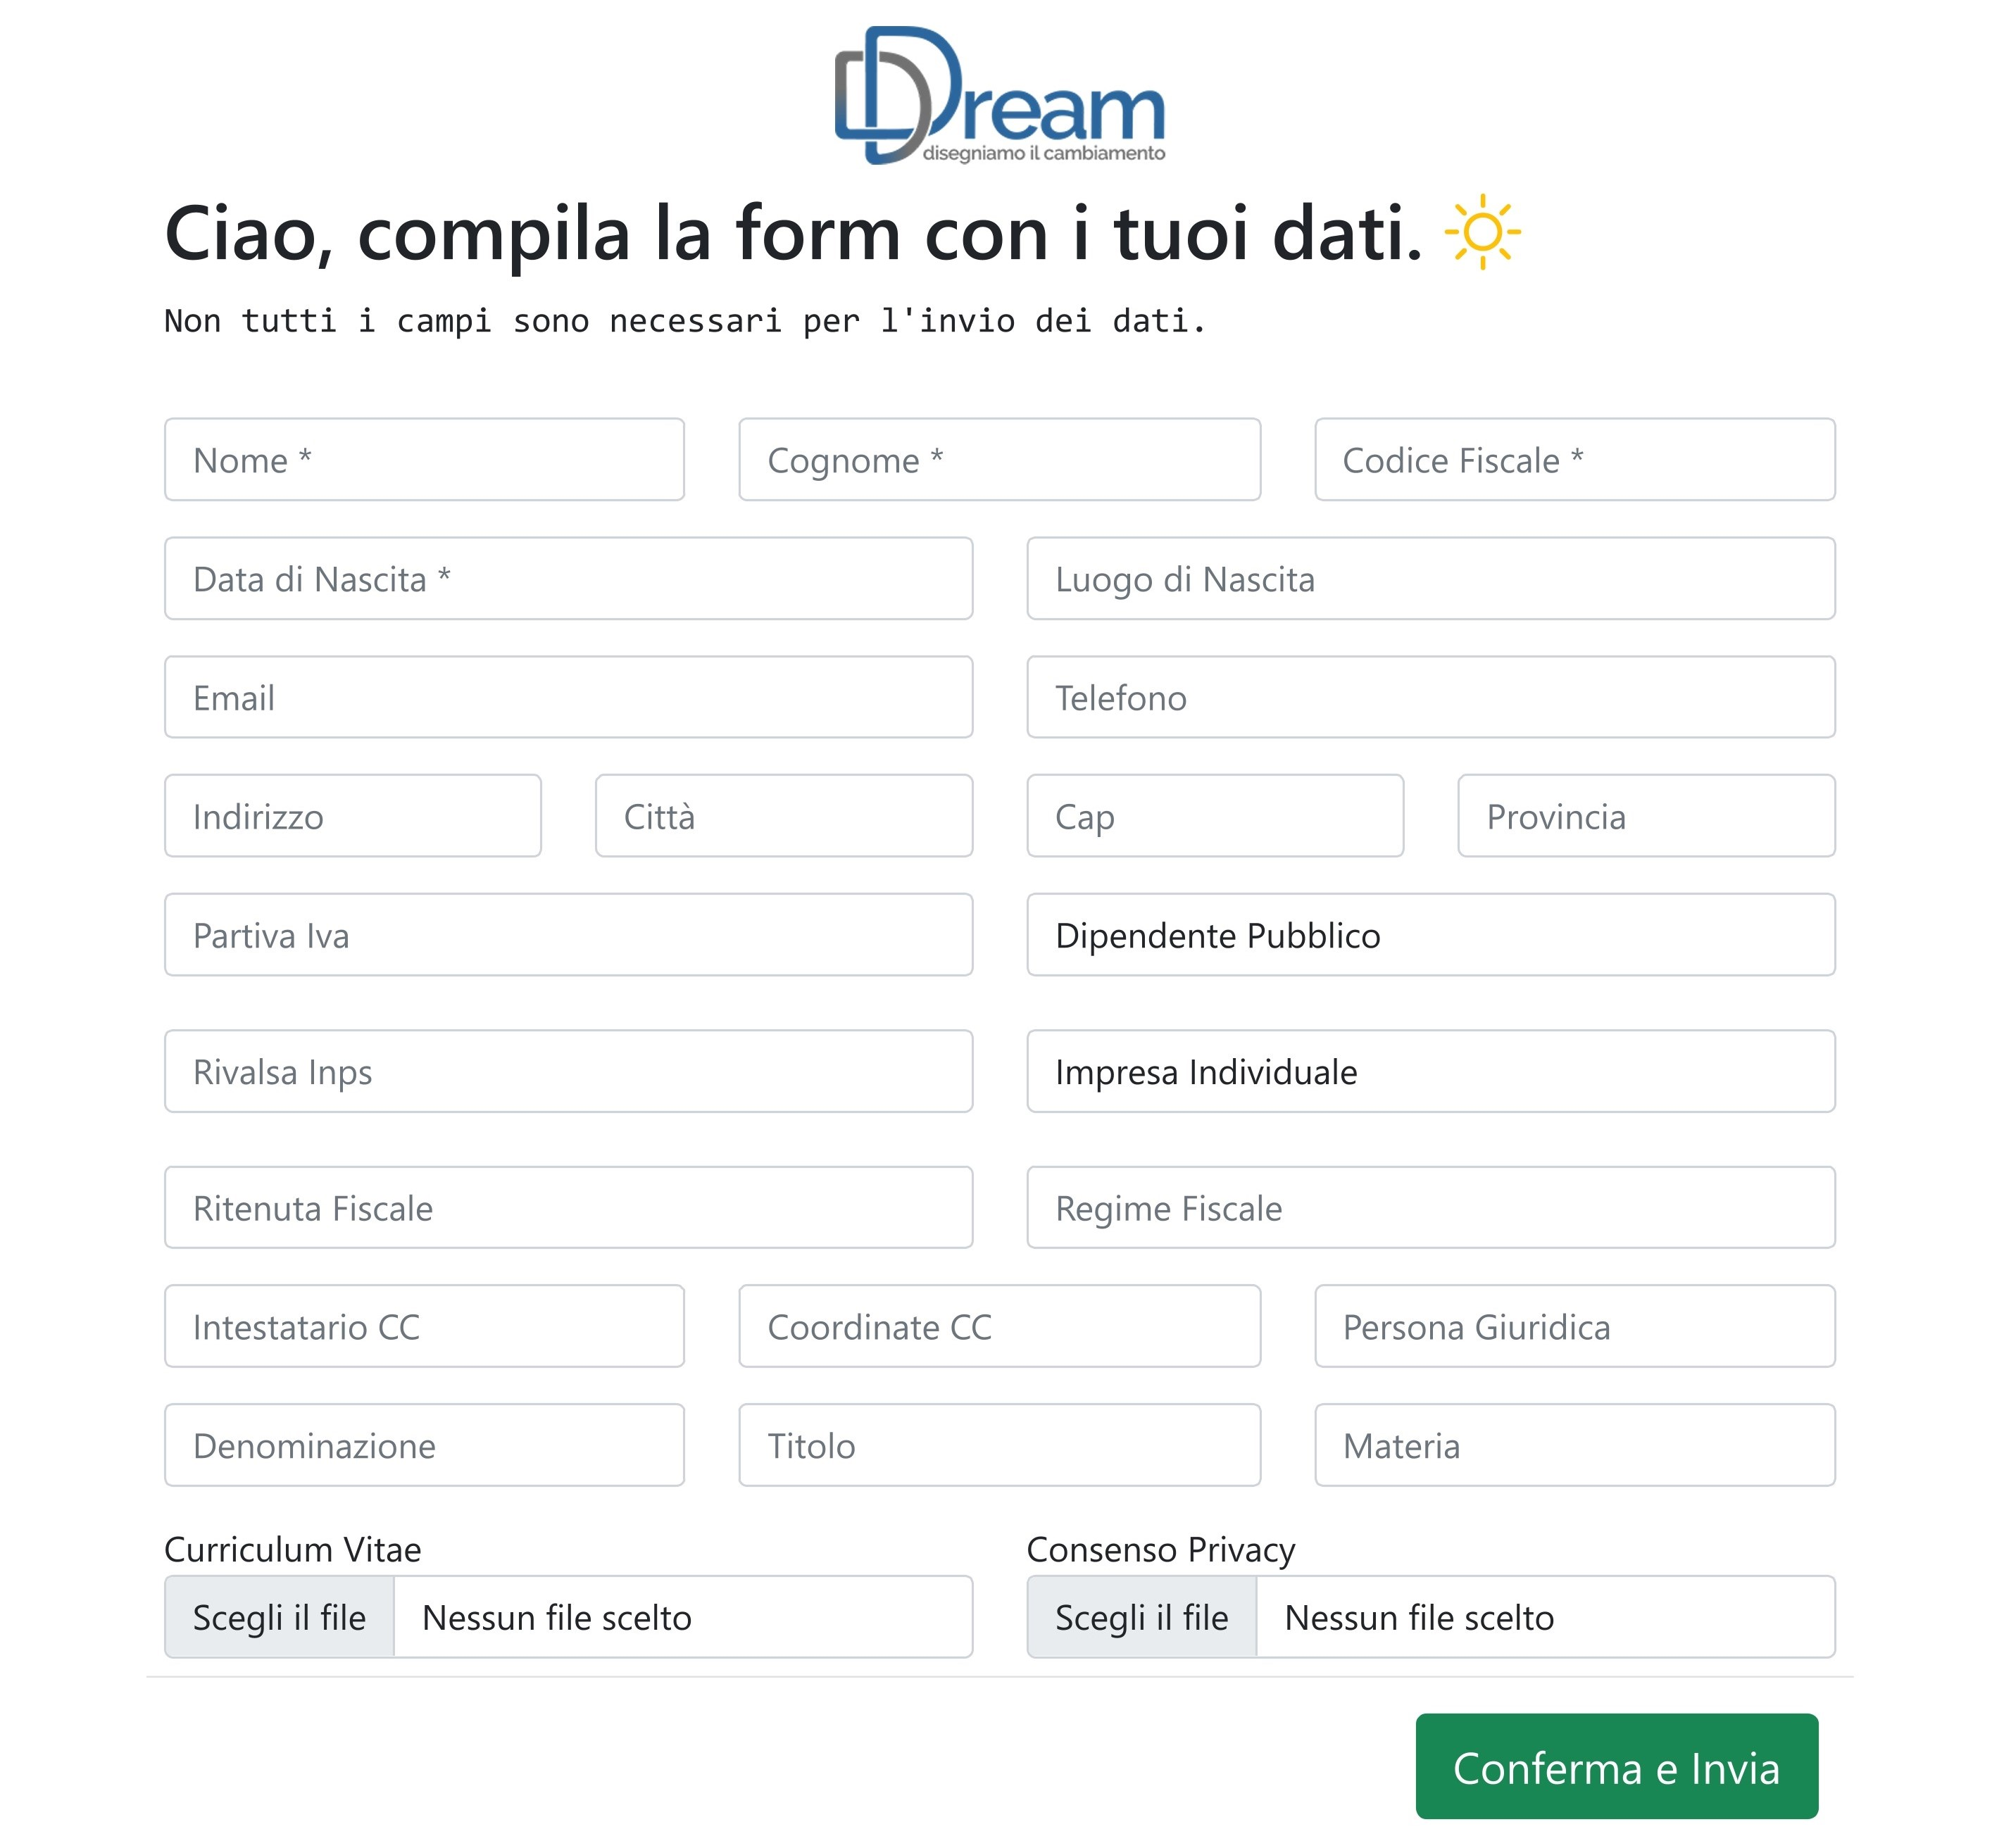
\includegraphics[scale=0.50]{img/screen/Public.jpg}
\caption{Pagina pubblica per risorse (screenshot)}
\label{fig:public}
\end{figure}
\clearpage
\newpage


    \chapter{Testing e validazione}
\label{cha:test}
La fase di testing consiste nella verifica del codice implementato tramite vari casi di test. In generale sono presenti due metodi di testing: l'analisi statica e l'analisi dinamica. Il primo tipo ricerca eventuali errori o comportamenti inaspettati senza eseguire il software stesso, ma solamente analizzandone il codice; la seconda metodologia consiste nella ricerca di malfunzionamenti del prodotto eseguendo il programma con vari input in ingresso prestabiliti. \\
L'analisi dinamica prevede due sottotipi di fasi di verifica e validazione: l'analisi funzionale, che si basa sulla quantità dei test effettuati, e quella strutturale, che invece considera la copertura del codice da testare.
Se quindi l'analisi funzionale ha lo scopo di sottoporre a una serie di casi di test il programma per verificare i requisiti definiti, l'analisi strutturale esegue una serie di casi di test al fine di verificare la maggior quantità possibile di righe di codice.\\

\begin{figure}[!hbt]
\centering
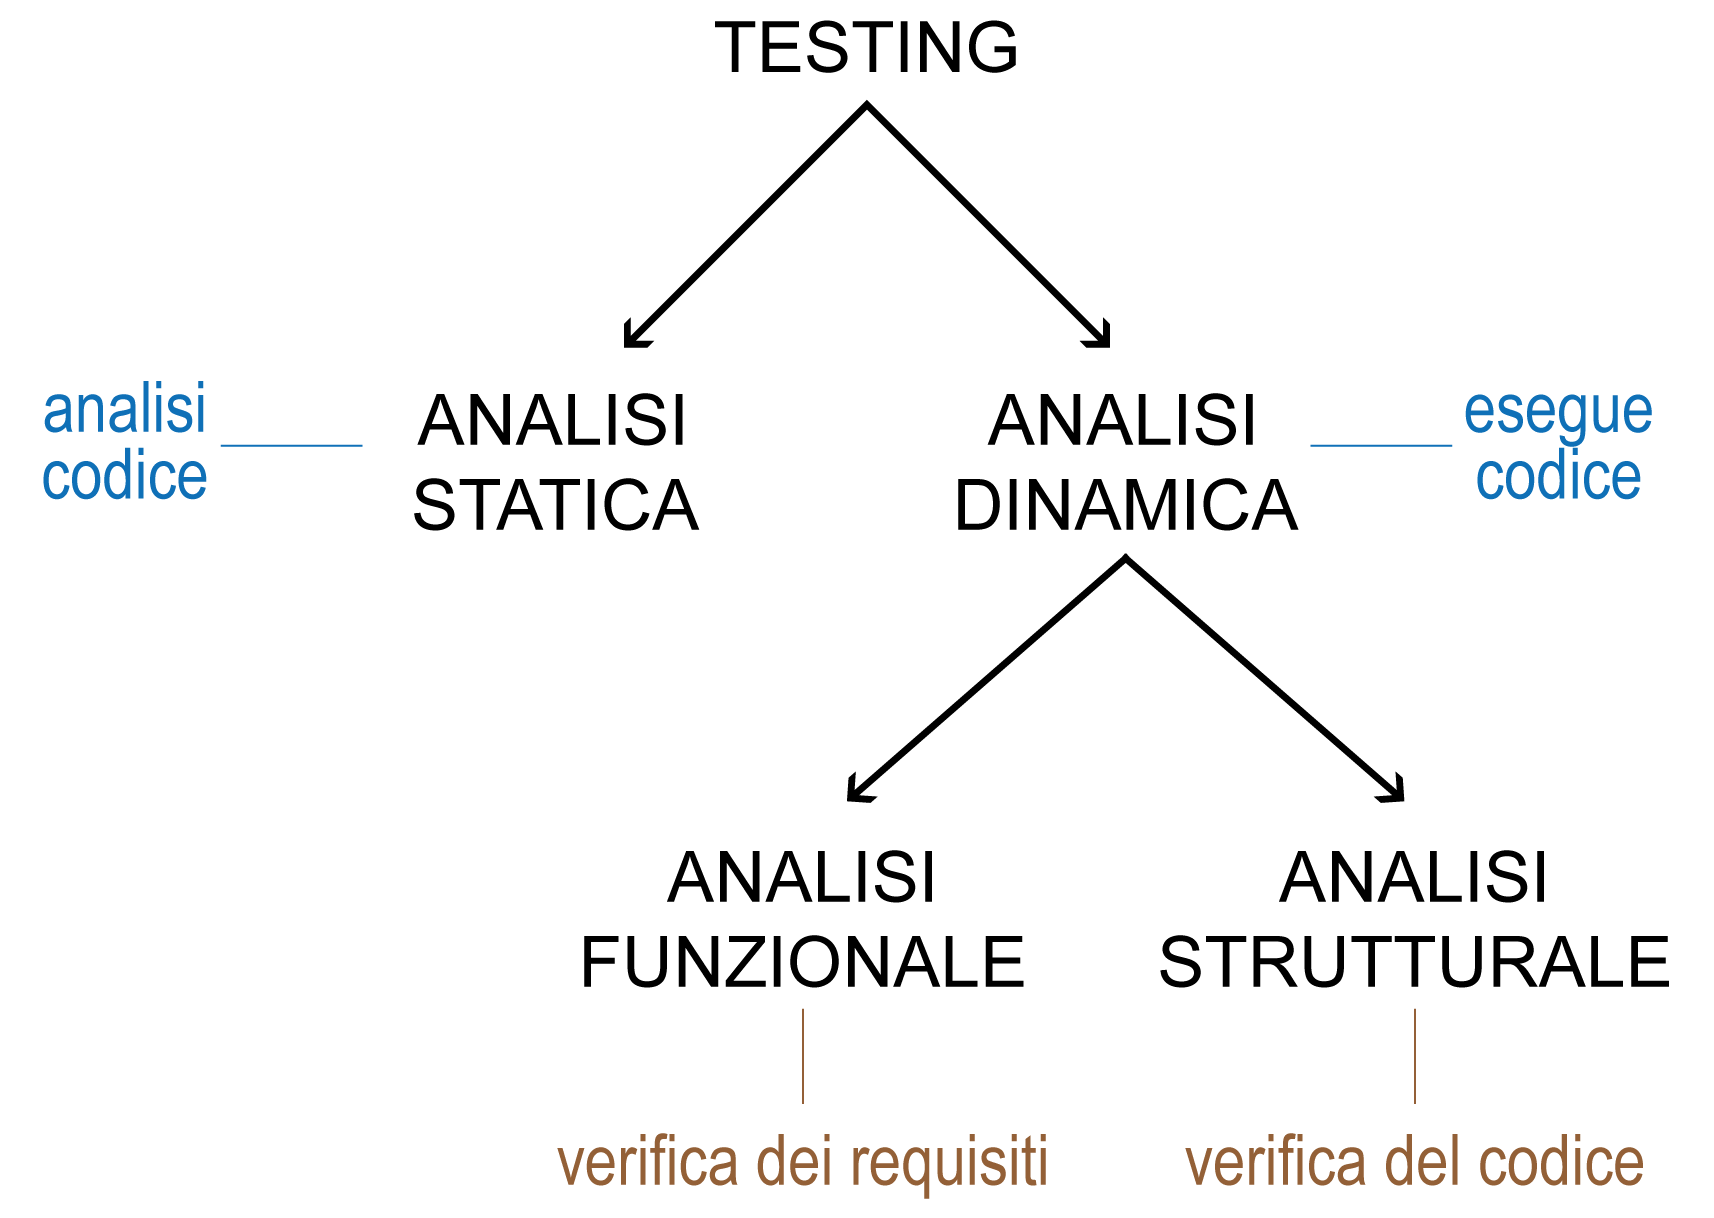
\includegraphics[scale=0.55]{img/testing.png}
\caption{I tipi di analisi del testing}
\label{fig:testing}
\end{figure}
\noindent
\newline
Un caso di test, per essere definito valido, deve avere un’alta probabilità di scoprire un errore, non essere ridondante, e garantire una verifica di giusta complessità.\\




\subsection{Testing con Jest}
\label{sec:jest}
Uno dei framework JavaScript più usati per il testing è Jest \cite{jest}, libreria che permette la creazione, l'esecuzione e la strutturazione dei test senza particolari configurazioni e include sia un test runner, che funzioni di asserzione. Fornisce anche una serie di funzionalità aggiuntive, come la ricerca automatica dei test da eseguire nel codice sorgente, l'esecuzione delle verifiche in parallelo o la possibilità di testare il codice asincrono in modo sincrono.\\
\newline
Nonostante non siano state elaborate verifiche tramite questa libreria durante il progetto, si riporta a titolo di esempio un possibile utilizzo per un test case banale \cite{jest_ex}. Il codice mostrato (listing \ref{code:jest}) presenta la funzione \verb|moltiplica| che riceve come parametri due numeri e ne effettua il prodotto, da questa si crea un file \verb|.js| contenente il test da verificare che, in questo caso, analizza la correttezza del risultato dell'operazione. Tramite Jest, dopo aver eseguito la prova, viene quindi restituito l'esito, positivo nel caso in cui il valore ritornato corrisponda alla corretta moltiplicazione e negativo viceversa con la prova che non viene considerata passata.

\begin{listing}[!hbt]
\begin{minted}{js}
//funzione moltiplica
function moltiplica(n1, n2) {
  return n1 * n2;
}
module.exports = moltiplica;

//creazione ed esecuzione test
const mul = require('./moltiplica');
test('mul 3 * 2 to equal 6', () => {
  expect(mul(3)(2)).toBe(6);
});

//risultato test
PASS  ./mul.test.js
OK mul 3 * 2 to equal 6 (5ms)
\end{minted}
\caption{Esempio di test con framework Jest}
\label{code:jest}
\end{listing}
\noindent



\subsection{Casi di test}
\label{sec:casi} 
Nonostante la fase di verifica tramite analisi dinamica non sia stata svolta tramite strumenti appositi, sono stati individuati vari test case verificati manualmente ispezionando le risposte di alcune funzioni critiche. Si riportano alcuni dei test effettuati relativi alla creazione dei profili utenti e di un'anagrafica (in questo caso quella dei \textit{Corsi} come esempio), illustrando precondizioni e risultato attesto, e riportandone il risultato effettivamente riscontrato.

\begin{table}[h!]
\centering
\begin{tabular}{|c|c|c|c|}
\hline
\multicolumn{1}{|c|}{\textbf{Caso di test}} & \multicolumn{1}{c|}{\textbf{Condizioni}} & \multicolumn{1}{|c|}{\textbf{Risultato Atteso}} & \multicolumn{1}{|c|}{\textbf{Risultato}}\\ \hline
Creazione di un account & \makecell{\textit{username} e\\ \textit{password}} &  \makecell{Il sistema crea l'account con le credenziali\\specificate e restituisce il messaggio \textit{OK}} &  \textit{OK} \\ \hline
\makecell{Creazione di un account\\senza specificare\\username e/o password} & --- & \makecell{Il sistema non crea l'account e restituisce\\il messaggio di errore \textit{err-user}} &  \textit{err-user} \\ \hline
\makecell{Creazione di un account\\senza rispettare\\i vincoli di password } & --- & \makecell{Il sistema non crea l'account e restituisce\\il messaggio di errore \textit{err-psw}} &  \textit{err-psw} \\ \hline

\end{tabular}
\caption{Casi di test su creazione account (tutti i test passati)}
\label{}
\end{table}

\begin{table}[h!]
\begin{center}
\begin{tabular}{|c|c|c|c|}
\hline
\multicolumn{1}{|c|}{\textbf{Caso di test}} & \multicolumn{1}{c|}{\textbf{Condizioni}} & \multicolumn{1}{|c|}{\textbf{Risultato Atteso}} & \multicolumn{1}{|c|}{\textbf{Risultato}}\\ \hline
Creazione di un corso & \makecell{campi\\obbligatori} &  \makecell{Il sistema crea il corso secondo i campi\\specificati e restituisce il messaggio \textit{OK}} &  \textit{OK} \\ \hline
\makecell{Creazione di un corso\\senza specificare tutti\\i campi obbligatori} & \makecell{---} & \makecell{Il sistema non crea il corso e restituisce\\il messaggio di errore \textit{err-corso}} &  \textit{err-corso} \\ \hline
\makecell{Eliminazione di un corso} & \makecell{vincoli di \\integrità\\rispettati}& \makecell{Il sistema elimina il corso e restituisce\\il messaggio \textit{OK}} &  \textit{OK} \\ \hline
\makecell{Eliminazione di un corso\\senza rispettare i\\vincoli di integrità} & \makecell{---} & \makecell{Il sistema non elimina il corso e restituisce\\il messaggio di errore \textit{err-contr}} &  \textit{err-contr}\\ \hline

\end{tabular}
\caption{Casi di test su creazione ed eliminazione corsi (tutti i test passati)}
\label{}
\end{center}
\end{table}


     \chapter{Conclusioni}
\label{cha:conclusioni}
Il presente elaborato ha riportato ogni fase della progettazione del software gestionale sviluppato a supporto dell'area formazione dell'azienda Dream S.R.L. Si è collocato il progetto in relazione ai temi della gestione dei processi e dei Sistemi Informativi, illustrata l'analisi dei requisiti raccolti e la costruzione del database. Infine si è mostrata la parte di programmazione dell'applicativo e i test effettuati.\\
\newline
Si presentano ora gli scenari futuri del lavoro realizzato e, nella seconda sezione, si descrivono le considerazioni finali. 

\section{Sviluppi futuri}
\label{sec:futuro}
Il gestionale sviluppato è attualmente utilizzato dagli utenti dell'organizzazione, e disponibile online. In intesa con l'azienda ho stabilito un accordo per gestire e implementare anche le nuove funzionalità che saranno richieste in futuro, e per correggere gli errori che emergeranno durante l'utilizzo. Grazie alla suite usata sarà possibile intervenire in modo semplice sul codice per aggiungere moduli al progetto e controllare il rilascio delle varie versioni.\\
\newline
L'obiettivo è quello di continuare l'implementazione del gestionale in modo chiaro e strutturato, considerando anche che i nuovi requisiti da soddisfare saranno probabilmente relativi all'ottimizzazione di altri processi dell'area aziendale.     

\section{Considerazioni personali}
\label{sec:personali}
Il periodo di tirocinio è stato sicuramente positivo e istruttivo. Ho avuto modo non solo di assimilare nuove nozioni tecniche e di rafforzare quelle già in mio possesso, ma soprattutto di svolgere molte nuove attività. Sono consapevole che le esperienze fatte e le conoscenze apprese mi saranno utili nel proseguimento del mio percorso formativo, indipendentemente dalle scelte future che intraprenderò.\newline
Se da un lato parte delle fasi di analisi e di sviluppo sono state un approfondimento delle nozioni viste in alcuni corsi accademici seguiti come quello di Ingegneria del Software o di Basi di Dati, dall'altro ho avuto modo di acquisire nuove competenze trasversali legate alla comunicazione, al lavoro di gruppo e, in generale, alle capacità relazionali. \\
\newline
Realizzare un progetto a trecentosessanta gradi è stata un'esperienza molto stimolante e mi ha permesso di conoscere e capire i processi aziendali presenti, nonché lavorare in team su progetti condivisi, ma anche svolgere le attività in autonomia quando necessario.\\
\newline
Avendo vissuto ogni fase con positività, curiosità e volontà di apprendimento, mi ritengo soddisfatto del tirocinio e della stesura di questo elaborato nella sua totalità.\\
Tutto ciò, unitamente al mio percorso triennale di studi, mi ha permesso di crescere come persona rendendomi pronto ad affrontare nuove sfide.

  
    
      
      
    \endgroup


    % bibliografia in formato bibtex
    %
    % aggiunta del capitolo nell'indice
    \addcontentsline{toc}{chapter}{Bibliografia}
    % stile con ordinamento alfabetico in funzione degli autori
    \bibliographystyle{plain}
    \bibliography{biblio}
%%%%%%%%%%%%%%%%%%%%%%%%%%%%%%%%%%%%%%%%%%%%%%%%%%%%%%%%%%%%%%%%%%%%%%%%%%
%%%%%%%%%%%%%%%%%%%%%%%%%%%%%%%%%%%%%%%%%%%%%%%%%%%%%%%%%%%%%%%%%%%%%%%%%%
%% Nota
%%%%%%%%%%%%%%%%%%%%%%%%%%%%%%%%%%%%%%%%%%%%%%%%%%%%%%%%%%%%%%%%%%%%%%%%%%
%% Nella bibliografia devono essere riportati tutte le fonti consultate 
%% per lo svolgimento della tesi. La bibliografia deve essere redatta 
%% in ordine alfabetico sul cognome del primo autore. 
%% 
%% La forma della citazione bibliografica va inserita secondo la fonte utilizzata:
%% 
%% LIBRI
%% Cognome e iniziale del nome autore/autori, la data di edizione, titolo, casa editrice, eventuale numero dell’edizione. 
%% 
%% ARTICOLI DI RIVISTA
%% Cognome e iniziale del nome autore/autori, titolo articolo, titolo rivista, volume, numero, numero di pagine.
%% 
%% ARTICOLI DI CONFERENZA
%% Cognome e iniziale del nome autore/autori (anno), titolo articolo, titolo conferenza, luogo della conferenza (città e paese), date della conferenza, numero di pagine. 
%% 
%% SITOGRAFIA
%% La sitografia contiene un elenco di indirizzi Web consultati e disposti in ordine alfabetico. 
%% E’ necessario:
%%   Copiare la URL (l’indirizzo web) specifica della pagina consultata
%%   Se disponibile, indicare il cognome e nome dell’autore, il titolo ed eventuale sottotitolo del testo
%%   Se disponibile, inserire la data di ultima consultazione della risorsa (gg/mm/aaaa).    
%%%%%%%%%%%%%%%%%%%%%%%%%%%%%%%%%%%%%%%%%%%%%%%%%%%%%%%%%%%%%%%%%%%%%%%%%%
%%%%%%%%%%%%%%%%%%%%%%%%%%%%%%%%%%%%%%%%%%%%%%%%%%%%%%%%%%%%%%%%%%%%%%%%%%
    

    % \titleformat{\chapter}
    %     {\normalfont\Huge\bfseries}{Allegato \thechapter}{1em}{}
    % % sezione Allegati - opzionale
    % \appendix
    % \chapter{Titolo primo allegato}

Lorem ipsum dolor sit amet, consectetur adipiscing elit. Donec sed nunc orci. Aliquam nec nisl vitae sapien pulvinar dictum quis non urna. Suspendisse at dui a erat aliquam vestibulum. Quisque ultrices pellentesque pellentesque. Pellentesque egestas quam sed blandit tempus. Sed congue nec risus posuere euismod. Maecenas ut lacus id mauris sagittis egestas a eu dui. Class aptent taciti sociosqu ad litora torquent per conubia nostra, per inceptos himenaeos. Pellentesque at ultrices tellus. Ut eu purus eget sem iaculis ultricies sed non lorem. Curabitur gravida dui eget ex vestibulum venenatis. Phasellus gravida tellus velit, non eleifend justo lobortis eget. 

\section{Titolo}
Lorem ipsum dolor sit amet, consectetur adipiscing elit. Donec sed nunc orci. Aliquam nec nisl vitae sapien pulvinar dictum quis non urna. Suspendisse at dui a erat aliquam vestibulum. Quisque ultrices pellentesque pellentesque. Pellentesque egestas quam sed blandit tempus. Sed congue nec risus posuere euismod. Maecenas ut lacus id mauris sagittis egestas a eu dui. Class aptent taciti sociosqu ad litora torquent per conubia nostra, per inceptos himenaeos. Pellentesque at ultrices tellus. Ut eu purus eget sem iaculis ultricies sed non lorem. Curabitur gravida dui eget ex vestibulum venenatis. Phasellus gravida tellus velit, non eleifend justo lobortis eget. 

\subsection{Sottotitolo}
Lorem ipsum dolor sit amet, consectetur adipiscing elit. Donec sed nunc orci. Aliquam nec nisl vitae sapien pulvinar dictum quis non urna. Suspendisse at dui a erat aliquam vestibulum. Quisque ultrices pellentesque pellentesque. Pellentesque egestas quam sed blandit tempus. Sed congue nec risus posuere euismod. Maecenas ut lacus id mauris sagittis egestas a eu dui. Class aptent taciti sociosqu ad litora torquent per conubia nostra, per inceptos himenaeos. Pellentesque at ultrices tellus. Ut eu purus eget sem iaculis ultricies sed non lorem. Curabitur gravida dui eget ex vestibulum venenatis. Phasellus gravida tellus velit, non eleifend justo lobortis eget. 


\chapter{Titolo secondo allegato}

Lorem ipsum dolor sit amet, consectetur adipiscing elit. Donec sed nunc orci. Aliquam nec nisl vitae sapien pulvinar dictum quis non urna. Suspendisse at dui a erat aliquam vestibulum. Quisque ultrices pellentesque pellentesque. Pellentesque egestas quam sed blandit tempus. Sed congue nec risus posuere euismod. Maecenas ut lacus id mauris sagittis egestas a eu dui. Class aptent taciti sociosqu ad litora torquent per conubia nostra, per inceptos himenaeos. Pellentesque at ultrices tellus. Ut eu purus eget sem iaculis ultricies sed non lorem. Curabitur gravida dui eget ex vestibulum venenatis. Phasellus gravida tellus velit, non eleifend justo lobortis eget. 

\section{Titolo}
Lorem ipsum dolor sit amet, consectetur adipiscing elit. Donec sed nunc orci. Aliquam nec nisl vitae sapien pulvinar dictum quis non urna. Suspendisse at dui a erat aliquam vestibulum. Quisque ultrices pellentesque pellentesque. Pellentesque egestas quam sed blandit tempus. Sed congue nec risus posuere euismod. Maecenas ut lacus id mauris sagittis egestas a eu dui. Class aptent taciti sociosqu ad litora torquent per conubia nostra, per inceptos himenaeos. Pellentesque at ultrices tellus. Ut eu purus eget sem iaculis ultricies sed non lorem. Curabitur gravida dui eget ex vestibulum venenatis. Phasellus gravida tellus velit, non eleifend justo lobortis eget. 

\subsection{Sottotitolo}
Lorem ipsum dolor sit amet, consectetur adipiscing elit. Donec sed nunc orci. Aliquam nec nisl vitae sapien pulvinar dictum quis non urna. Suspendisse at dui a erat aliquam vestibulum. Quisque ultrices pellentesque pellentesque. Pellentesque egestas quam sed blandit tempus. Sed congue nec risus posuere euismod. Maecenas ut lacus id mauris sagittis egestas a eu dui. Class aptent taciti sociosqu ad litora torquent per conubia nostra, per inceptos himenaeos. Pellentesque at ultrices tellus. Ut eu purus eget sem iaculis ultricies sed non lorem. Curabitur gravida dui eget ex vestibulum venenatis. Phasellus gravida tellus velit, non eleifend justo lobortis eget. 




\end{document}
